%% Master's thesis, Master's Programme in Computer Science, University of Helsinki.
%% Written on the CSM thesis template (HYthesisML.cls) of the Department of
%% Computer Science; see CSM-thesis-template_2021_09_07/ for the pristine copy.

% STEP 1: language, pagination, programme, and study track.
% openright is passed through to report so chapters start on a right-hand page;
% the template's own default is openany.
% a4paper has to be given here: the template sets it with a \PassOptionsToClass
% placed after \documentclass, by which time report is already loaded, so the
% stock template silently produces US Letter pages.
\documentclass[english,twoside,openright,a4paper,censored,csm,software-track-2020]{HYthesisML}

\usepackage{csquotes}

% REFERENCES: numeric (Vancouver) style, one of the three styles the template
% offers. sorting=none keeps the numbers in citation order, as IEEEtran did.
\usepackage[style=numeric,bibstyle=numeric,backend=biber,natbib=true,
            sorting=none,sortcites=true,maxbibnames=99,giveninits=true,uniquename=init]{biblatex}
\addbibresource{bibliography.bib}
% List the authors in the bibliography as Lastname F.
\DeclareNameAlias{sortname}{family-given}
% Without a mark of its own the bibliography keeps the last chapter's title in
% the running head of its continuation pages.
\defbibheading{bibliography}[\bibname]{%
  \chapter*{#1}%
  \markboth{#1}{#1}}

% lmodern, textcomp, color, graphicx, epsfig, subfigure, tikz, amsmath, amssymb,
% caption, titlesec and appendix are all loaded by the class itself.
\usepackage[pdftex, plainpages=false]{hyperref} % For hyperlinks and pdf metadata
\usepackage{fancyhdr} % For nicer page headers
\usetikzlibrary{arrows.meta, positioning, automata, shapes.geometric, calc, fit, backgrounds}
%\usepackage{wrapfig} % For nice text-wrapping figures (use at own discretion)
\usepackage{array} % Ragged-right p-columns in the Chapter 6 tables
\usepackage{float} % [H] placement for tables that must not drift past their section
\usepackage{listings} % For the side-by-side C++/Rust excerpts in Chapter 6

% Ragged-right paragraph column: avoids stretched inter-word spacing in narrow cells.
\newcolumntype{R}[1]{>{\raggedright\arraybackslash}p{#1}}

% listings has no built-in Rust definition.
\lstdefinelanguage{Rust}{
  morekeywords={as,break,const,continue,crate,dyn,else,enum,extern,false,fn,for,
    if,impl,in,let,loop,match,mod,move,mut,pub,ref,return,self,Self,static,struct,
    super,trait,true,type,unsafe,use,where,while},
  sensitive=true,
  morecomment=[l]{//},
  morecomment=[s]{/*}{*/},
  morestring=[b]",
}

\lstdefinestyle{thesiscode}{
  basicstyle=\ttfamily\scriptsize,
  keywordstyle=\bfseries,
  commentstyle=\itshape\color[gray]{0.45},
  stringstyle=\color[gray]{0.35},
  numbers=none,
  frame=none,
  breaklines=true,
  showstringspaces=false,
  columns=fullflexible,
  keepspaces=true,
  xleftmargin=0pt,
  aboveskip=1pt,
  belowskip=1pt,
}
\lstset{style=thesiscode}

\onehalfspacing %line spacing
%\singlespacing
%\doublespacing

%\fussy 
\sloppy % sloppy and fussy commands can be used to avoid overlong text lines

% STEP 2:
% Set up all the information for the title page and the abstract form.
% Replace parameters with your information.
\title{Performance, Safety, and Engineering Trade-offs of Rust and C++ in Nokia RAN Control-Plane Systems}
\author{Ha Vien}
\date{\today}
% Supervisors are printed on the abstract form rather than on the title page.
% The template asks for an academic title in front of each name; the two Nokia
% instructors are listed untitled by their own preference.
\supervisors{Prof. Keijo Heljanko, Christoph Luneburg, Petteri Kotimaa}
% Examiners are assigned by the faculty. The first is known; the second is not
% yet named, so the field carries only the name that is settled. The class
% prints examiners nowhere, so nothing here reaches the page in either case,
% and an unfilled second name cannot leak into a submitted PDF.
\examiners{Prof. Keijo Heljanko}
\keywords{Rust, C++, RAN control plane, tail latency, memory safety, fault injection, incremental adoption}
% Where deposited fills itself in from the class. Additional information is the
% study track, taken from the software-track-2020 class option.
\additionalinformation{\translate{\track}}


\classification{\protect{\ \\
\  Software and its engineering $\rightarrow$ Software notations and tools $\rightarrow$ General programming languages\  \\
\  Computer systems organization $\rightarrow$ Real-time systems $\rightarrow$ Real-time system specification\\
\  Networks $\rightarrow$ Network types $\rightarrow$ Mobile networks
}}

% if you want to quote someone special. You can comment this line and there will be nothing on the document.
%\quoting{Bachelor's degrees make pretty good placemats if you get them laminated.}{Jeph Jacques} 


% OPTIONAL STEP: Set up properties and metadata for the pdf file that pdfLaTeX makes.
% But you don't really need to do this unless you want to.
\hypersetup{
    %bookmarks=true,         % show bookmarks bar first?
    unicode=true,           % to show non-Latin characters in Acrobat’s bookmarks
    pdftoolbar=true,        % show Acrobat’s toolbar?
    pdfmenubar=true,        % show Acrobat’s menu?
    pdffitwindow=false,     % window fit to page when opened
    pdfstartview={FitH},    % fits the width of the page to the window
    pdftitle={Performance, Safety, and Engineering Trade-offs of Rust and C++ in Nokia RAN Control-Plane Systems},
    pdfauthor={Ha Vien},
    pdfsubject={Master's thesis, Computer Science},
    pdfcreator={Ha Vien},
    pdfproducer={pdfLaTeX}, % producer of the document
    pdfkeywords={Rust} {C++} {RAN control plane} {tail latency} {memory safety},
    pdfnewwindow=true,      % links in new window
    colorlinks=true,        % false: boxed links; true: colored links
    linkcolor=black,        % color of internal links
    citecolor=black,        % color of links to bibliography
    filecolor=magenta,      % color of file links
    urlcolor=cyan           % color of external links
}

% Campaign summary numbers (representative load, saturation knee, repeat count, ...)
% are generated by bench/plot_figures.py together with the figures and tables, so the
% prose cannot drift out of step with the data it describes.
% Generated by bench/plot_figures.py -- do not edit by hand.
\newcommand{\ReprLoad}{28}
\newcommand{\ReprLoadAch}{28.0}
\newcommand{\ReprLoadShortfall}{0.1}
\newcommand{\SatKnee}{334}
\newcommand{\TrackingLoad}{336}
\newcommand{\NRepeats}{20}
\newcommand{\NLoadLevels}{14}
\newcommand{\NVariants}{4}
\newcommand{\NRuns}{1120}
\newcommand{\PNineNineSpread}{14}
\newcommand{\PFiftySpread}{2.9}
\newcommand{\PFiftyRange}{3}
\newcommand{\PNineNineRange}{460}
\newcommand{\PNineNineMaxCI}{2540}
\newcommand{\MaxOfferedLoad}{784}
\newcommand{\NTests}{10}
\newcommand{\MinAttainableP}{0.0000019}
\newcommand{\CorrectedFloor}{0.000019}
\newcommand{\NSignificant}{2}
\newcommand{\SmallestHolm}{0.00010}
\newcommand{\NExclZero}{4}
\newcommand{\NTailExclZero}{1}
\newcommand{\TailExclZeroRows}{p99 latency under system}
\newcommand{\RobustExclZeroRows}{p50 latency, Peak RSS and CPU utilisation under system}
\newcommand{\PFiftyDiffAbsMax}{1.6}
\newcommand{\PFiftyDiffCIMax}{3}
\newcommand{\RssLangDiffLo}{1.3}
\newcommand{\RssLangDiffHi}{1.7}
\newcommand{\RssLangCILo}{-0.5}
\newcommand{\RssLangCIHi}{1.9}
\newcommand{\CpuDiffAbsMax}{3.4}
\newcommand{\CrossAllocConsistent}{p50 latency, p99 latency, p99.9 latency, Peak RSS and CPU utilisation}
\newcommand{\CrossAllocReversed}{none}
\newcommand{\NCrossAllocReversed}{0}
\newcommand{\RssAllocDiffLo}{55.9}
\newcommand{\RssAllocDiffHi}{56.5}
\newcommand{\BudgetRepeats}{15}
\newcommand{\BudgetCoreCpp}{34.4}
\newcommand{\BudgetCoreRust}{21.3}
\newcommand{\BudgetSvcCpp}{13.52}
\newcommand{\BudgetSvcRust}{12.63}
\newcommand{\BudgetHandoffCpp}{13.49}
\newcommand{\BudgetHandoffRust}{12.61}
\newcommand{\BudgetCoreShareMax}{0.250}
\newcommand{\BudgetCoreFaster}{Rust}
\newcommand{\BudgetCoreRatio}{1.6}
\newcommand{\BudgetHandoffSlower}{C++}
\newcommand{\BudgetBoundVsCore}{101}
\newcommand{\FfiCrossing}{2.54}
\newcommand{\FfiOpRepeats}{15}
\newcommand{\FfiOpNative}{12.3}
\newcommand{\FfiOpSeam}{12.7}
\newcommand{\FfiOpDelta}{+192}
\newcommand{\FfiOpDeltaLo}{-954}
\newcommand{\FfiOpDeltaHi}{+1341}
\newcommand{\FfiOpP}{0.239}
\newcommand{\FfiOpBoundPct}{10.91}


% A measured value above its bootstrap 95% confidence interval. The interval is
% printed in full rather than as a symmetric half-width because a bootstrap
% interval on the median of a heavy-tailed latency sample is markedly asymmetric.
% [t] so the median's baseline lines up with the row label and the interval
% hangs beneath it, rather than the pair straddling the label.
\newcommand{\mci}[3]{%
  \begin{tabular}[t]{@{}r@{}}%
    $#1$\\[-2pt]{\scriptsize$[#2,\,#3]$}%
  \end{tabular}}

% Size and cyclomatic-complexity proxies for the two cores, measured by
% bench/complexity.py with one tool applied identically to both languages.
% Generated by bench/complexity.py -- do not edit by hand.
\newcommand{\CppFuncs}{37}
\newcommand{\RustFuncs}{40}
\newcommand{\CppNloc}{511}
\newcommand{\RustNloc}{608}
\newcommand{\CppCcnTotal}{93}
\newcommand{\RustCcnTotal}{79}
\newcommand{\CppCcnMean}{2.5}
\newcommand{\RustCcnMean}{2.0}
\newcommand{\CppCcnMax}{13}
\newcommand{\RustCcnMax}{6}
\newcommand{\CppCcnMaxFn}{\texttt{worker\_loop}}
\newcommand{\RustCcnMaxFn}{\texttt{add\_drb}}
\newcommand{\CcnTotalDrop}{15}
\newcommand{\NlocRise}{19}


% Artefact-level measurements that belong to no campaign: record sizes from the
% compiled probes, parity-suite coverage, the size of the conformance campaign,
% and the size of the FFI seam. Generated by bench/artefact_facts.py so that a
% number in the prose cannot outlive the code it describes.
% Generated by bench/artefact_facts.py -- do not edit by hand.
\newcommand{\CppUeCtxBytes}{96}
\newcommand{\RustUeCtxBytes}{88}
\newcommand{\UeCtxGapBytes}{8}
\newcommand{\CppUeCtxStatePad}{3}
\newcommand{\CppUeCtxKeyEnd}{50}
\newcommand{\CppUeCtxKeyPad}{6}
\newcommand{\CppRequestBytes}{160}
\newcommand{\RustRequestBytes}{96}
\newcommand{\SignalingMsgBytes}{68}
\newcommand{\SweepUes}{5\,000}
\newcommand{\UeCtxGapTotalKB}{40}
\newcommand{\CppQueueResidentMB}{1.3}
\newcommand{\RustQueueResidentMB}{0.8}
\newcommand{\CppLineCov}{94.4}
\newcommand{\RustLineCov}{97.9}
\newcommand{\RustRegionCov}{99.1}
\newcommand{\ConfHandOps}{223}
\newcommand{\ConfGenOps}{9\,000}
\newcommand{\FfiSeamLines}{231}
\newcommand{\FfiHeaderLines}{67}
\newcommand{\FfiEntryPoints}{11}
\newcommand{\FfiUnsafeFns}{9}
\newcommand{\DeadlockTsanHits}{3}
\newcommand{\DeadlockTsanRuns}{12}
\newcommand{\FaultClasses}{14}
\newcommand{\FaultClassesPrevented}{7}
\newcommand{\FaultClassesBoundary}{7}
\newcommand{\FaultClassesUndetected}{4}
\newcommand{\LostUpdateExpected}{40\,000}
\newcommand{\LostUpdateRustHandled}{28\,714}
\newcommand{\LostUpdateRustLost}{11\,286}
\newcommand{\LostUpdateCppHandled}{27\,320}
\newcommand{\LostUpdateCppLost}{12\,680}
\newcommand{\CppTestBinaries}{6}
\newcommand{\RustTests}{27}


% Keep the contents page to chapters, sections, and subsections. The \paragraph
% headings inside sections are running signposts, often a full sentence long,
% and listing all of them turns the contents into a second outline that competes
% with the real one. titlesec ignores \setcounter{tocdepth} for these levels, so
% they are dropped where they are typeset instead.
\makeatletter
\renewcommand*\l@paragraph[2]{}
\makeatother

\begin{document}

% Generate title page.
\maketitle

% STEP 3:
% Write your abstract (of course you really do this last).
% You can make several abstract pages (if you want it in different languages)
% by repeating the otherlanguage environment with a different language.

% The abstract form is a fixed 12 cm box that also has to hold the CCS paths, so
% it is set single-spaced as in the template; the 1.5 spacing of the body would
% cost it a fifth of its lines. Overflow is neither clipped nor reported: it
% overprints the keyword rows, so keep this to 31 typeset lines and look at
% page 3 after editing.
{\singlespacing
\begin{otherlanguage}{english}
\begin{abstract}
\noindent\textbf{Context.}
Radio Access Network (RAN) control planes are written mostly in C++ for performance, at a
well-known cost in memory safety and concurrency. Rust promises comparable performance with
compile-time safety, but its fit for this latency-critical setting is unproven.

\noindent\textbf{Objective.}
The thesis compares modern C++ and Rust on a UE Context Management service modelled on a real
Nokia gNB-CU-CP component. Average-throughput comparisons leave four dimensions open: tail latency
and jitter under overload, the C++ defect classes Rust prevents at compile time, the overhead of
its safety model, and the cost of incremental adoption.

\noindent\textbf{Methods.}
One language-agnostic specification is frozen first, then implemented twice with identical
algorithms, concurrency model, allocator, and build settings. A synthetic workload is swept to
overload, both versions pass the same parity tests, and the evaluation adds fault injection and an
FFI prototype.

\noindent\textbf{Results.}
Safe Rust rejects all five injected memory-safety and data-race defect classes at compile
time. In C++ the same five build cleanly and show up only at runtime, if a sanitiser catches
them. Five further classes fail in both languages. On two of them C++ tooling reports what
Rust does not. The seam to C++ leaves the core \texttt{unsafe}-free and costs at most
$\FfiOpBoundPct\%$ of one operation. Performance changes at saturation. Below it median
latency matches, yet an end-to-end call spends only $\BudgetCoreShareMax\%$ on language
work. Cross-thread handoff takes the rest, so the sweep reflects the design more than the
language. Timed alone, Rust's operation is $\BudgetCoreRatio\times$ faster and the process
is a few MiB larger. Above saturation the order flips: \OverloadSustainedFaster{} holds
$\OverloadThrRatio\times$ the throughput of \OverloadSustainedSlower{} in \OverloadThrAgree{}
interleaved repeats with both allocators. The far tail below saturation cannot be settled
on a virtualised host.

\noindent\textbf{Conclusions.}
The main cost of adopting Rust is engineering effort and the learning curve, not run-time
performance at nominal load. The gain is freedom from data races, not from concurrency
defects in general. Overload narrows that claim: a service that must degrade gracefully
depends on the standard library's synchronisation primitives, not on the safety model, and
a nominal-load test would not expose the gap.
\end{abstract}
\end{otherlanguage}
}

% The class's \mytableofcontents switches straight to arabic numbering, which is
% right when the contents are the last thing before the body. The lists of
% figures and tables sit in between, so the front matter is numbered in roman
% here and \mainmatter starts the body at arabic 1.
\cleardoublepage
\pagenumbering{roman}
\setcounter{page}{1}
\tableofcontents

% \cleardoublepage has to come before \addcontentsline: the \chapter* inside \listoffigures
% opens a new page itself, so the contents entry must record the page after that, not before.
% The entries themselves are the short forms of the captions, \caption[short]{full}.
\cleardoublepage
\phantomsection
\addcontentsline{toc}{chapter}{\listfigurename}
\listoffigures

\cleardoublepage
\phantomsection
\addcontentsline{toc}{chapter}{\listtablename}
\listoftables

% Flush the last roman-numbered page before \mainmatter switches to arabic, or the
% reset lands on the still-open List of Tables page and the body starts at 3 instead of 1.
\cleardoublepage

\mainmatter

% -----------------------------------------------------------------------------------
% STEP 4: Write the thesis.
% Your actual text starts here. You shouldn't mess with the code above the line except
% to change the parameters. Removing the abstract and ToC commands will mess up stuff.
\chapter{Introduction}

Mobile networks are moving from specialised hardware to software on ordinary servers.
Functions that once ran on fixed-purpose, vertically integrated equipment are now
re-implemented as programs on general-purpose machines. The Radio Access Network (RAN),
long the most hardware-bound part of the stack, is part of that shift.

In 5G, the base station (gNB) is split into a central unit and one or more distributed
units. The central unit is split again into control- and user-plane
functions~\cite{3gpp38401,3gpp38300}. Open-RAN pushes the same idea further: the RAN
becomes virtualised, multi-vendor software linked by open
interfaces~\cite{polese2023oran}. The control plane that results, the gNB-CU-CP, is a
large, stateful, highly concurrent program. It tracks every connected device, runs RRC
signalling~\cite{3gpp38331}, and coordinates mobility and handovers, all within strict
latency limits.

Load at a busy site is high. A single site can run thousands of connection-management and
mobility procedures per second, each with a budget of a few
milliseconds~\cite{3gpp38913}. A deployed control plane may track millions of active
devices at once. As the RAN moves to cloud-native, disaggregated deployments, the
correctness, reliability, and timing of this software increasingly set the quality of the
whole network. An outage or a tail-latency spike here is not a local defect. Every device
the site serves is affected~\cite{dean2013tail,barroso2017microseconds}.

This control-plane software is, today, written mostly in C++. The choice is a
rational one: C++ offers the low-level control, mature tooling, and performance that
latency-critical systems demand. But that performance comes with a well-known cost. C++
places the burden of memory and concurrency management on the programmer, and decades of
experience show that this burden is routinely mishandled, producing use-after-free errors,
double-frees, data races, and related defects that are expensive to find, dangerous in
production, and responsible for a large share of security vulnerabilities in industry
practice~\cite{msrc2019memory,google2022android}. Rust has emerged as the first mainstream
systems language to promise an escape from this trade-off: memory safety and data-race
freedom enforced at compile time, with performance intended to be competitive with
C++~\cite{klabnik2023rust,jung2018rustbelt}. Whether that promise holds for a
telecom-grade, latency-critical control plane, where predictability under overload matters
as much as raw speed, is not well understood. This thesis, carried out at Nokia, addresses
the question directly: it develops two functionally equivalent implementations of a
representative RAN subsystem, a UE Context Management service modelled on a real Nokia
gNB-CU-CP component, in modern C++ and in Rust, and compares them under a realistic
synthetic signalling workload.

\section{Key terms and abbreviations}
For readers outside the telecom domain, Table~\ref{tab:abbrev} fixes the abbreviations and terms
used throughout the thesis. Three of them recur constantly. The \emph{gNB-CU-CP} is the
control-plane software this work is about. \emph{UE Context Management (UECM)} is the specific
subsystem reimplemented and measured. \emph{Tail latency} (the p99/p99.9 percentiles rather than
the mean) is the property that, more than average speed, decides whether such a system meets its
deadlines~\cite{dean2013tail,barroso2017microseconds}.

\begin{table}[H]
\centering
\caption[Abbreviations and key terms]{Abbreviations and key terms used throughout the thesis.\label{tab:abbrev}}
% Single-spaced: the class's text block is 23cm, and at the body's 1.5 spacing a
% glossary of this length runs past the bottom of the page. The opened row
% height keeps it legible at single spacing.
\singlespacing
\renewcommand{\arraystretch}{1.25}
\begin{tabular}{@{}p{0.21\linewidth} p{0.71\linewidth}@{}}
\hline\hline
Term & Meaning \\
\hline
RAN & Radio Access Network: the part of the mobile network connecting devices to the core \\
NG-RAN & Next-Generation RAN, the 5G radio-access-network architecture \\
IMT-2030 & The ITU framework for the generation after 5G, commonly called 6G \\
AI-RAN & An architecture in which AI and RAN workloads share one accelerated infrastructure \\
gNB & 5G base station (``next-generation NodeB'') \\
gNB-CU / DU & Central Unit / Distributed Unit: the disaggregated halves of a gNB \\
gNB-CU-CP & Control-plane part of the central unit: the system class studied here \\
UE & User Equipment: an end device (phone, modem) attached to the network \\
UECM & UE Context Management: the per-UE state-management subsystem reimplemented here \\
RRC & Radio Resource Control: the control-plane signalling protocol between UE and gNB \\
DRB & Data Radio Bearer: a per-UE user-plane data channel set up during a session \\
Control plane & The signalling and management path, as opposed to the user-plane data path \\
Tail latency & High-percentile latency (p99, p99.9), the worst-case-oriented timing metric \\
Jitter & How much latency varies from one operation to the next, as opposed to its typical value \\
Saturation & The offered load beyond which the service can no longer keep up and requests start queueing \\
Shard & One of several independent slices of the UE state, each owned by exactly one worker thread \\
FFI & Foreign Function Interface: calling Rust from C++ across a C ABI \\
HDR histogram & High-Dynamic-Range histogram, used for accurate latency capture \\
\hline
\end{tabular}
\end{table}

\section{Motivation and industrial context}
Three trends make this comparison timely. The first is the cloud-native evolution of the RAN
itself. Moving control-plane functions onto general-purpose servers raises, rather than
lowers, the premium on software quality: the software is longer-lived, evolves continuously,
runs at higher concurrency, and must meet its deadlines without the determinism that
purpose-built hardware once provided. This shift is accelerated by Open-RAN disaggregation,
which turns the base station into virtualised, multi-vendor software connected by open
interfaces~\cite{polese2023oran}, so that the control plane a vendor ships increasingly
competes on software-engineering quality (reliability, predictable timing, security, and the
ease with which a large codebase can be evolved safely) and no longer on purpose-built hardware. In
this setting a latency regression or a memory-corruption defect is not a localised bug but a
network-wide reliability and security risk, and a language-selection question stops being
academic and becomes a concrete engineering decision.

The second trend is that AI is moving from a tool used to tune the network into a workload the
network is built to carry, and the next generation is being specified that way from the start.
IMT-2030, the ITU framework for 6G, lists artificial intelligence and communication among its
six usage scenarios and ubiquitous intelligence among its four design
principles~\cite{itu2023imt2030}. The architecture forming around that is AI-RAN, in which
telecommunications and AI workloads are orchestrated together on shared, accelerated
infrastructure, so the sites that run the radio also host distributed edge AI
platforms~\cite{polese2026airan}. The AI-RAN Alliance states the operational requirement
directly: one common infrastructure has to run both kinds of workload concurrently, and their
service-level agreements may differ~\cite{airan2025orchestrator}. That changes what a language
choice has to buy for a control plane. Its software no longer has the host to itself. It
contends for CPU, memory, and cache with inference work whose arrival pattern it does not
control, and a co-tenant that takes capacity away lowers the load at which the control plane
saturates. Saturation is where the two languages separate most sharply in the measurements of
Chapter~\ref{chapter:eval}. Memory footprint and behaviour past that point are becoming
selection criteria in their own right, and neither is settled by the architecture above the
code.

The third trend is an industry-wide shift toward memory-safe languages. Large
software organisations report that the majority of their serious security vulnerabilities
stem from memory-safety errors, and that adopting memory-safe languages measurably reduces
them~\cite{msrc2019memory,google2022android,vanderstoep2025android,google2024securebydesign}.
The case no longer rests on vendor reporting alone: a group spanning academia and industry has
argued that memory safety now needs standardised terminology and requirements if it is to be
specified and procured at all~\cite{watson2025memorysafety}. This concern has risen to the level of national
policy: cybersecurity agencies now urge software manufacturers to publish ``memory-safe
roadmaps'' and to migrate away from memory-unsafe languages such as C and
C++~\cite{cisa2023memorysafe,oncd2024building}. In the market this subsystem is sold into it has
also become a regulatory matter. The EU Cyber Resilience Act places secure-by-design and
lifecycle vulnerability-handling obligations on manufacturers of products with digital elements,
with the vulnerability-reporting obligations applying from September 2026 and most of the
remainder from December 2027~\cite{eu2024cra}. It names no programming language, and it would be wrong to read it as
requiring one. What it changes is that the recurring defect classes of a memory-unsafe language
become a compliance exposure as well as an engineering one. Rust in particular has moved from a niche
language into operating-system kernels, cloud infrastructure, and increasingly into
telecommunications. Production hypervisors such as AWS Firecracker, which underpins its
serverless platform, are already written in Rust~\cite{agache2020firecracker}. Yet the evidence base for Rust's suitability rests largely on
general-purpose software and on average-case performance benchmarks. The specific question a
telecom vendor must answer, whether Rust can meet the tail-latency and predictability
requirements of a RAN control plane, whether it genuinely prevents the defect classes that
plague the existing C++ code, and what it costs to adopt it incrementally inside a large C++
codebase, has not been answered with direct, controlled evidence. Providing such evidence
for a representative subsystem is the motivation for this work.

\paragraph{Industrial setting.}
This thesis is carried out at Nokia, one of the small number of vendors that build, maintain,
and evolve production RAN software end to end. That market is concentrated in very few hands:
the five largest suppliers took 96\% of worldwide RAN revenue over the first three quarters of
2025, with concentration by Herfindahl--Hirschman Index at a ten-year
high~\cite{delloro2025ran3q,delloro2026ran}. The subsystem it studies, UE Context
Management (UECM), is modelled on a real gNB-CU-CP control-plane component rather than a
textbook example.

The gNB-CU-CP is not a minor component. In the 3GPP disaggregated architecture it is the
control-plane half of the central unit: it hosts RRC and manages the UE context lifecycle,
delegating user-plane bearer handling to the CU-UP over the E1
interface~\cite{3gpp38401,3gpp38300,3gpp38331,3gpp38463}. It does so under the
millisecond-scale procedure budgets the 5G system places on control
signalling~\cite{3gpp38913}, and at the very high event rates and connected-device counts a
deployed network sustains. Because it is written in C++, it inherits both that language's
performance and its memory-safety and concurrency hazards. That is precisely where the three
trends above converge.

Software of this class is shipped, evolved, and operated across live operator networks. A
language-selection decision here is therefore a concrete production concern rather than a
hypothetical one, which is what makes a controlled comparison on a representative subsystem
valuable to a vendor.

UECM is a deliberate choice of study object within that setting. It is small enough to
reimplement faithfully and to reason about in full, yet it exercises exactly the properties
that make RAN control-plane code hard: per-UE mutable state, a strict operation lifecycle,
high concurrency across many UEs, and hard tail-latency expectations. Conclusions drawn from
it therefore transfer to the broader class of stateful, concurrent control-plane services.
They also remain reproducible by readers outside Nokia, because the implementation is driven
entirely by a public, frozen specification rather than by proprietary code.

\paragraph{A decision with a generational horizon.}
A language choice in software of this class is not revisited often, and it outlives the
generation it was made for. The next generation is being specified now: 3GPP has allocated
Release 20 to the 6G studies and Release 21 to the normative work, against a calendar set by the
ITU radiocommunication sector that asks for technology proposals in early 2029 and the submitted
specifications by mid-2030~\cite{itu2023imt2030,3gpp2024road6g}. That work explicitly covers
migration from and interworking with 5G, so a control plane written for the current generation is
not retired when the next one arrives but maintained alongside it. The practical question for a
vendor is therefore not only which language suits a 5G control plane today, but which one it can
still afford to be maintaining a decade from now.

Nothing in the next generation's stated objectives relaxes the requirements that motivate this
comparison. The IMT-2030 framework names security and resilience as one of four design principles common to
all of its usage scenarios, states that the system is expected to be secure by design, and
defines resilience as the ability to keep operating correctly during and after a disruptive
event. It also carries the ultra-reliable low-latency scenario forward in strengthened form, as
hyper-reliable and low-latency communication~\cite{itu2023imt2030}. Freedom from whole classes of
defect and predictable behaviour when the system is disturbed are thus being written into the
objectives of the next generation rather than left to implementers, and both depend on the
language and its libraries as much as on the architecture above them.

The policy clock falls inside the same window, and the roadmap expectation noted above carries a
date keyed to precisely this horizon. CISA and the FBI classify the development of new product
lines in a memory-unsafe language as a bad practice that significantly elevates risk where the
product serves critical infrastructure and a memory-safe alternative is available. They also expect
manufacturers of existing products to publish a memory-safety roadmap, exempting only products
whose announced support ends before January 2030~\cite{cisa2025badpractices}. Mobile-network infrastructure sits squarely inside that
scope, and the Cyber Resilience Act obligations described above are in full force from December
2027~\cite{eu2024cra}. A vendor that defers the language question until the next generation is
specified will not thereby have avoided making it. It will have made it by default, in the
incumbent language, for another decade of deployments.

What this thesis contributes to that decision is bounded, and the boundary is worth stating
plainly. The measurements here are taken on a subsystem modelled on a current-generation
component and evaluated against requirements that are already published. No claim is made about
requirements that have not yet been written. What crosses the generational boundary is not a
latency figure but the language-level comparison itself: which defect classes a compiler can rule
out, what the safety model costs, and what incremental adoption inside a large C++ codebase
involves. Those questions have the same answers whichever generation the specification above them
names, and they are cheapest to answer before the next codebase is started rather than after.

\paragraph{A concrete failure mode.}
To make the stakes concrete, consider a mobility storm in which many UEs hand over at once. A
single mishandled pointer, a UE context freed on release while an in-flight signalling message
still references it, produces a use-after-free. In C++ this compiles cleanly and may pass
ordinary testing, only to corrupt an unrelated UE's state or crash the worker thread under
precisely the high-concurrency conditions the system exists to handle. The same latent race
can equally show up as an unpredictable tail-latency spike instead of an outright crash. In
safe Rust the same design does not compile: ownership and borrowing reject the dangling
reference at build time. This one scenario captures why the thesis measures both
\emph{safety} (which defects are prevented, and when) and \emph{predictability} (tail
latency under overload) rather than average throughput alone.

\section{Problem statement}
Two properties of this domain make the language choice consequential. First, manual memory and
concurrency management in C++ exposes the software to defects such as use-after-free,
double-free, data races, and iterator invalidation, which are silent at compile time and costly
to find and fix at telecom scale. Second, what governs whether RAN deadlines are met is not
average throughput but worst-case and tail behaviour under load and
overload~\cite{dean2013tail}, a property that is easy to regress and hard to measure correctly.
Rust promises to remove the first class of defect at compile time while claiming performance
competitive on the second, but that claim rests mostly on general-purpose benchmarks rather
than on stateful, concurrent, latency-critical telecom workloads.

Bringing these threads together, the concrete problem this thesis addresses is the following.
Telecom vendors are under growing pressure, both technical and increasingly regulatory, to adopt
memory-safe languages, yet for the RAN control plane they lack \emph{direct, controlled}
evidence on which to base that decision. It is not established whether a Rust implementation of
a stateful, concurrent control-plane subsystem can match modern C++ in \emph{tail latency and
predictability under overload} (as opposed to average throughput), whether Rust's compile-time
guarantees actually eliminate the specific defect classes that affect the existing C++ code,
and what incremental adoption \emph{costs} inside a large C++ codebase. The available evidence
is largely general-purpose and average-case~\cite{balasubramanian2017rust,qin2020rust}, leaving
these three questions (predictability, prevented-defect scope, and migration cost) open for a
representative subsystem. Answering them under controlled, reproducible conditions is the
problem this thesis sets out to solve.

\section{Research questions and hypotheses}\label{sec:rqs}
The thesis is organised around four research questions, ordered to put predictability and
migration ahead of raw average performance:

\begin{description}
  \item[RQ1] How do Rust and modern C++ compare in latency predictability (median, p99
        and p99.9 tail latency, and the maximum) for a RAN control-plane workload under
        increasing load and overload?
  \item[RQ2] Which classes of memory-safety and concurrency defects that occur in C++ are
        eliminated at compile time in the Rust implementation, and at what stage and cost
        are the remaining ones detected?
  \item[RQ3] What is the overhead, if any, of Rust's safety model (bounds checks,
        ownership-driven copies, abstraction cost) on throughput, CPU utilisation, and
        memory behaviour?
  \item[RQ4] What are the practical implications (effort, FFI interoperability, and risk)
        of adopting Rust incrementally within an existing C++ RAN software ecosystem?
\end{description}

The questions are approached with three prior expectations, stated here so that the evaluation
can confirm or refute them instead of merely describing results after the fact. \textbf{H1:} for
this workload the two languages are performance-equivalent in the operationally relevant region
below saturation, with any difference confined to the far tail. \textbf{H2:} safe Rust prevents
at compile time the memory-safety and concurrency defect classes that C++ leaves to
best-effort, after-the-fact detection. \textbf{H3:} the run-time cost of C++-to-Rust
interoperability is negligible relative to the cost of the operations invoked, so that the true
cost of incremental adoption is engineering effort rather than performance. H2 is stated so that
it can fail. The defect catalogue behind RQ2 spans classes safe Rust is expected to prevent and
classes it is expected not to, so the study can locate the boundary of the guarantee instead of
only confirming it. These hypotheses are revisited against the evidence in
Section~\ref{sec:hypotheses}.

\section{Contributions, results, and limitations}
The thesis makes five contributions. Two are artifacts: a reproducible benchmarking framework
for telecom control-plane workloads, and a frozen shared specification with two parity-tested
implementations of a RAN control-plane subsystem, one in C++ and one in Rust. Two are results:
a quantitative comparison that weighs tail latency and predictability alongside average
throughput, and a defect-class taxonomy from controlled fault injection that marks where Rust's
compile-time guarantee stops. The fifth is a set of engineering and migration guidelines for
language selection in cloud-native RAN evolution (Section~\ref{sec:guidelines}).

The findings divide three ways. On \emph{safety} (RQ2), every injected memory-safety and
data-race defect class is prevented at compile time in safe Rust. The same defects all compile
in C++, and each is caught, if at all, only at run time and only under the right sanitiser. Five
boundary classes were chosen deliberately, and neither language prevents them. On two of those
the C++ tooling is ahead. On \emph{migration} (RQ4), the FFI seam is small and keeps the core
free of \texttt{unsafe}. Measured against the same operation called natively it costs at most
$\FfiOpBoundPct\%$ of one operation, so the real adoption cost is API design and not run-time
overhead. Both of these results are final.

On \emph{performance} (RQ1, RQ3) the answer divides at saturation, and drawing that division
correctly is part of the contribution. Below saturation the two implementations cannot be told
apart end to end at the median, and the far tail cannot be resolved on the available host. That
null is less informative than it looks. An end-to-end operation here is only
$\BudgetCoreShareMax\%$ language work and the rest is a cross-thread handoff, so the sweep bounds
the design and not the language. Measured on its own, the operation is
$\BudgetCoreRatio\times$ faster in Rust, while the Rust process holds a few MiB more resident
memory under both allocators. Past saturation the ordering reverses. The C++ build sustains
$\OverloadThrRatio\times$ the throughput of the Rust build, and uses more CPU for each completed
operation.

Four limitations bound all of this: a synthetic workload, one simplified subsystem,
single-author implementation bias, and a virtualised measurement host.
Chapter~\ref{chapter:discussion} treats each in detail.

The scope is drawn deliberately to protect the internal validity of the language comparison. In
scope are the UE Context Management functionality of Chapter~\ref{chapter:context}, the
shared-nothing concurrency design, the load sweep to overload, the fault-injection catalogue,
and the FFI prototype. Explicitly out of scope are the full gNB system and its remaining
control-plane domains, PHY/L2 processing and the data-heavy user plane, real captured traffic
traces (as opposed to a spec-justified synthetic workload), managed-language alternatives
(excluded on the tail-latency grounds argued in Chapter~\ref{chapter:background}), and
production deployment and operational concerns such as upgrade, observability, and
multi-tenancy. These exclusions trade external validity for the controlled conditions a fair
language comparison needs, and each is revisited as a limitation in
Chapter~\ref{chapter:discussion}.

\section{Significance and beneficiaries}
The results are intended to be directly actionable. For RAN vendors and cloud-native network
operators, the thesis supplies controlled evidence on the question that gates any language
decision. That question is not ``is Rust fast on average?'' but ``does Rust hold its tail latency and
predictability under overload, and what does incremental adoption cost?'', answered for a subsystem
representative of production control-plane code. For the standards and policy discussion around
memory-safe roadmaps~\cite{cisa2023memorysafe,oncd2024building}, it grounds a general mandate in
a concrete telecom data point. For the research community, the frozen specification, the
parity-tested implementations, the reproducible benchmarking framework, and the defect-class
taxonomy form a reusable baseline for further language and systems studies. And for practising
engineers, the fault catalogue and the migration prototype double as worked examples of what
Rust's guarantees do and do not buy in this domain.

\chapter{Background: Systems Languages for Latency-Critical Software\label{chapter:background}}
% The class prints the chapter and section titles in the running head in capitals,
% where the full title of this chapter runs into the margin.
\chaptermark{Background}

\section{RAN control-plane systems and the gNB-CU-CP}
The NG-RAN architecture splits the gNB into a central unit (gNB-CU) and distributed units,
with the control plane (gNB-CU-CP) handling RRC and connection management for each
UE~\cite{3gpp38401,3gpp38300,3gpp38331}. Such control-plane systems must satisfy demanding
non-functional requirements: very high event rates (UE mobility, signalling storms), strict
and predictable latency bounds that the 5G service and RAN specifications quantify as
KPIs~\cite{3gpp38913,3gpp22261}, long-lived software with continuously evolving complexity,
and heavily concurrent workloads. In these systems the worst-case and tail behaviour,
rather than the average, determines whether deadlines are met, which motivates the
predictability focus of this thesis.

Functionally, the gNB is disaggregated along two independent axes. The first is a
\emph{central/distributed} split: a central unit (gNB-CU) hosts the higher layers of the
protocol stack, while one or more distributed units (gNB-DU) host the lower, more
time-critical layers close to the radio. The second is a \emph{control/user-plane} split
inside the central unit, separating the control-plane function (gNB-CU-CP) from the
user-plane function (gNB-CU-UP). These parts communicate over standardised
interfaces: NG towards the 5G core, F1 between the CU and the DU, and E1 between the CU-CP and
the CU-UP~\cite{3gpp38401,3gpp38300,3gpp38463}. Open-RAN initiatives standardise these interfaces
further so that each part can be supplied by a different vendor and run as software on
commodity hardware~\cite{polese2023oran}. Figure~\ref{fig:ngran} places the subsystem studied
in this thesis, UE Context Management (UECM), inside the gNB-CU-CP: it owns the per-UE
control-plane state and mediates the RRC signalling and mobility procedures, which is why its
correctness and timing behaviour are representative of the control plane as a whole.

\begin{figure}
\centering
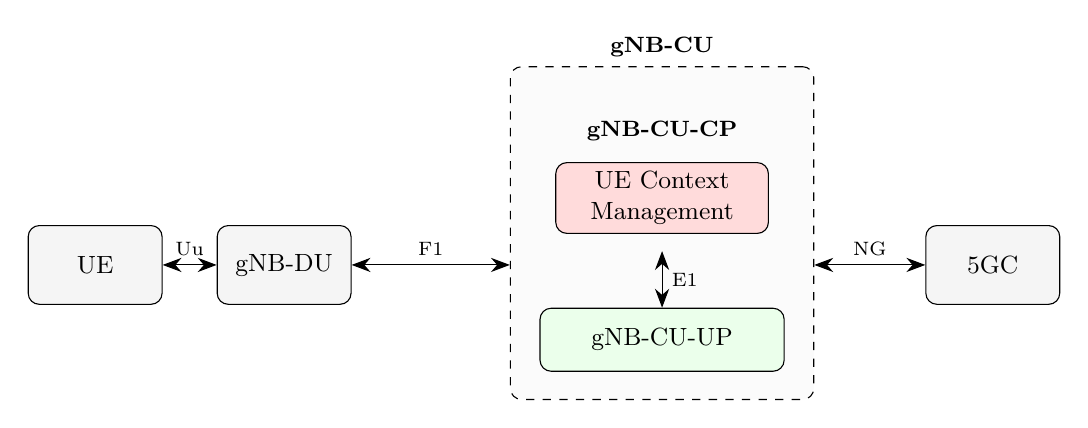
\begin{tikzpicture}[
    font=\small, >={Stealth[length=2.4mm]},
    box/.style={draw, rounded corners, minimum height=1.0cm, minimum width=1.7cm,
                align=center, fill=gray!8},
    cpbox/.style={draw, rounded corners, align=center, fill=blue!8},
    upbox/.style={draw, rounded corners, minimum width=3.1cm, minimum height=0.8cm,
                  align=center, fill=green!8},
    uecm/.style={draw, rounded corners, minimum width=2.7cm, minimum height=0.62cm,
                 fill=red!14, align=center}
  ]
  \node[box] (ue) at (0,0)   {UE};
  \node[box] (du) at (2.4,0) {gNB-DU};

  % Control plane, with UE Context Management shown nested inside it
  \node[font=\footnotesize\bfseries] (cpttl) at (7.2,1.7) {gNB-CU-CP};
  \node[uecm] (uecm) at (7.2,0.85) {UE Context\\ Management};
  \begin{scope}[on background layer]
    \node[cpbox, fit=(cpttl)(uecm), inner sep=6pt] (cp) {};
  \end{scope}
  % User plane
  \node[upbox] (up) at (7.2,-0.95) {gNB-CU-UP};

  \begin{scope}[on background layer]
    \node[draw, dashed, rounded corners, fill=gray!3,
          fit=(cp)(up), inner sep=10pt, label={[font=\footnotesize\bfseries]above:gNB-CU}] (cu) {};
  \end{scope}

  \node[box] (core) at (11.4,0) {5GC};

  \draw[<->] (ue) -- node[above,font=\scriptsize]{Uu} (du);
  \draw[<->] (du.east)         -- node[above,font=\scriptsize]{F1} (cu.west |- du);
  \draw[<->] (cu.east |- core) -- node[above,font=\scriptsize]{NG} (core.west);
  \draw[<->] (cp.south) -- node[right,font=\scriptsize]{E1} (up.north);
\end{tikzpicture}
\caption[Where the studied subsystem sits in the 5G NG-RAN]{Where the studied subsystem sits in the 5G NG-RAN. The gNB is split into a
distributed unit (gNB-DU) and a central unit (gNB-CU), and the central unit is split again
into control-plane (gNB-CU-CP) and user-plane (gNB-CU-UP) functions, connected by the
standardised F1, E1, and NG interfaces. UE Context Management (highlighted) is the per-UE
control-plane state manager inside the gNB-CU-CP that this thesis reimplements and
measures.\label{fig:ngran}}
\end{figure}

\section{Latency, throughput, and predictability in real-time software}\label{sec:predictability}
\sectionmark{Latency and predictability}
Latency-critical systems are judged less by how much work they do on average than by how
\emph{predictably} they do it. Three metrics must be distinguished. \emph{Throughput} is the
sustained rate of completed operations; \emph{latency} is the time an individual operation
takes; and \emph{jitter} is the variability of that latency. A system can have
excellent mean latency and still miss deadlines often. The meaningful figures are therefore the
high-percentile \emph{tail} latencies, the 99th (p99) and 99.9th (p99.9) percentiles, rather
than the mean. At the scale of a network, tail latency dominates user-visible behaviour: when
a single user action fans out into many internal operations, the slowest of them sets the
response time, so rare per-operation delays become common per-request delays~\cite{dean2013tail}.
Modern data-centre and networking software increasingly operates in a regime where the
relevant latencies are measured in microseconds, a range in which conventional
operating-system and software overheads are no longer negligible~\cite{barroso2017microseconds}.
Fine-grained measurement studies show that, even at moderate utilisation, hardware, operating-system,
and application-level effects such as background interference, scheduling, interrupt routing, and
power-saving states inflate the tail far beyond what queueing models predict~\cite{li2014tales}.
Figure~\ref{fig:tailconcept} sets the two effects side by side: the distance between the median
and the high percentiles, and the fan-out that turns a delay which is rare per operation into
one that is common per procedure.

\begin{figure}
\centering
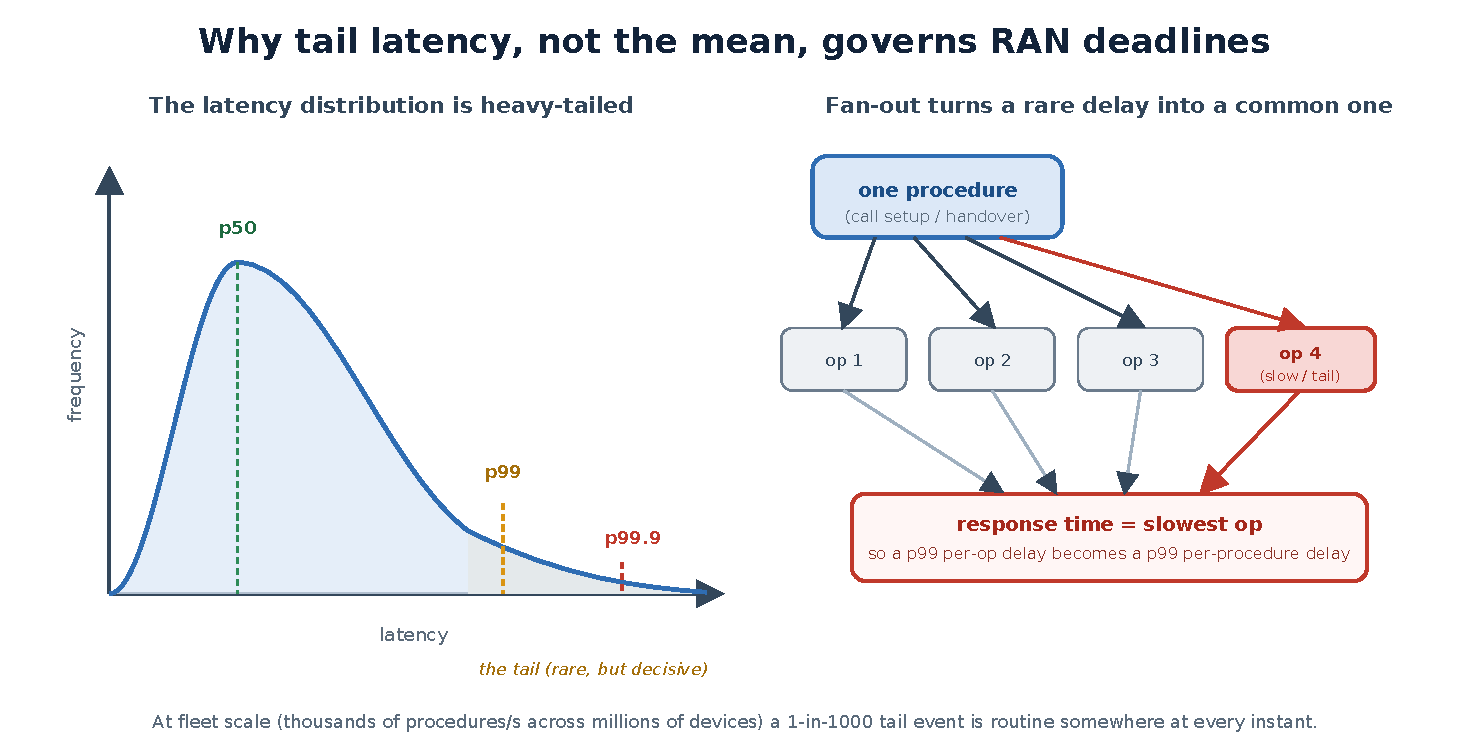
\includegraphics[width=\linewidth]{diagrams/pdf/11_tail_latency_concept.pdf}
\caption[Why the tail, not the mean, governs RAN deadlines]{Why the tail, not the mean, governs RAN deadlines. The latency distribution is
heavy-tailed (left), so the p99/p99.9 percentiles lie far from the median. Because a single
procedure fans out into many dependent operations whose slowest member gates completion (right),
a delay that is rare per operation becomes common per procedure. At fleet scale a one-in-a-thousand
tail event is routine somewhere at every instant.\label{fig:tailconcept}}
\end{figure}

Real-time systems are conventionally graded by the consequence of a missed deadline: in
\emph{hard} real-time a miss is a failure, in \emph{firm} real-time a late result is useless
but not catastrophic, and in \emph{soft} real-time a miss merely degrades quality. A RAN
control plane is best seen as soft-to-firm real-time: an occasional late signalling response
degrades service rather than endangering it, but at fleet scale and under signalling storms
such degradations accumulate into a network-wide reliability problem. This is compounded by
queueing behaviour: as offered load approaches service capacity, queueing delay grows
sharply and the latency tail explodes near saturation. Characterising a system therefore
requires driving it not just at nominal load but \emph{into overload}, which is why the
evaluation in this thesis sweeps load up to and beyond the saturation point.

Measuring tail latency correctly is itself a pitfall. A naive closed-loop load generator
that waits for each response before issuing the next request suffers \emph{coordinated
omission}: when the system stalls, the generator stalls with it and simply fails to record
the many requests that would have arrived during the stall, systematically hiding the very
tail it is meant to expose. Figure~\ref{fig:coord} contrasts the two generator models.
The distinction beneath this is a modelling one, not an
implementation detail. In a closed system a new request is triggered only by the completion of a
previous one, whereas in an open system arrivals are independent of completions, and the two
produce systematically different response-time behaviour on the same service process, with the
closed model reporting the lower figures~\cite{schroeder2006openclosed}. Sound measurement
therefore requires an open-loop model with an
intended schedule, correction for coordinated omission, high-dynamic-range latency histograms
that retain resolution across many orders of magnitude, and statistically rigorous reporting
with repeated runs and confidence intervals rather than single point
estimates~\cite{georges2007rigorous}. These techniques are applied in
Chapter~\ref{chapter:eval}.

\begin{figure}
\centering
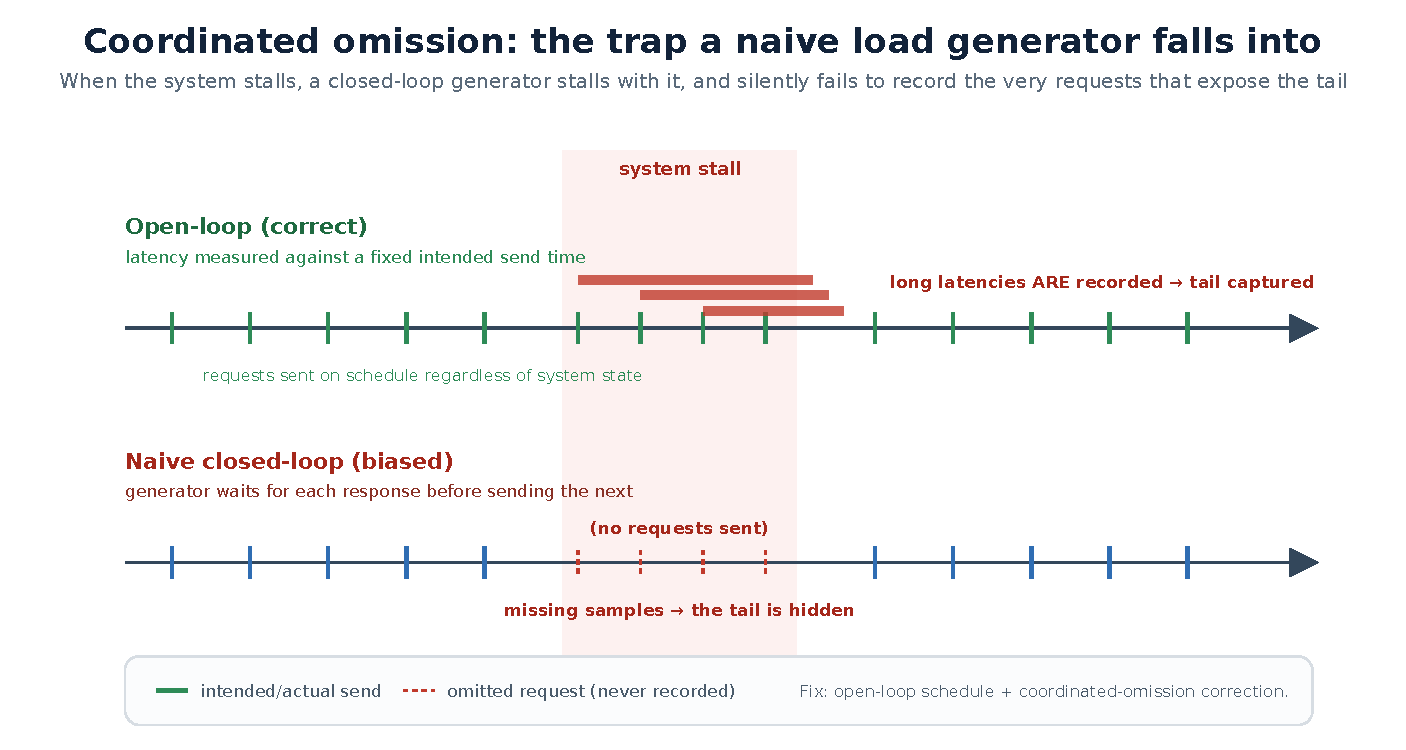
\includegraphics[width=\linewidth]{diagrams/pdf/16_coordinated_omission.pdf}
\caption[Coordinated omission under open- and closed-loop load]{Coordinated omission. An open-loop generator (top) sends on a fixed intended schedule
regardless of system state, so requests issued during a stall are recorded with their full
latency and the tail is captured. A naive closed-loop generator (bottom) waits for each response
before sending the next, so when the system stalls it stalls too and never issues the delayed
requests, silently omitting exactly the samples that would expose the tail.\label{fig:coord}}
\end{figure}

\section{C++ for latency-critical systems}\label{sec:cpplatency}
C++ is the default language for RAN control-plane software for good reasons. It offers
zero-overhead abstractions, direct control over memory layout and allocation, deterministic
destruction through the Resource Acquisition Is Initialization (RAII) idiom, and mature
compilers, libraries, and profiling tools, all without a garbage collector that could inject
unpredictable pauses. Modern C++ (C++11 and later) adds smart pointers
(\texttt{std::unique\_ptr}, \texttt{std::shared\_ptr}) that automate ownership, move semantics
that avoid needless copies, and a formal memory model with \texttt{std::atomic} for
lock-based and lock-free concurrency. These features make it possible to write fast and, with
discipline, reasonably safe systems code.

The difficulty is that safety in C++ remains the programmer's responsibility rather than a
property the compiler enforces. RAII and smart pointers reduce temporal errors without
eliminating them. Raw pointers and references can outlive the objects they point to, iterators can be
invalidated by container mutation, objects can be used after a move, and nothing in the type
system prevents a mutable object from being aliased and mutated concurrently from several
threads. The result is a well-known catalogue of defects (use-after-free, double-free,
buffer overflow, data races, deadlocks, and iterator invalidation) that are easy to
introduce and expensive to find at telecom scale. Memory-corruption errors of this kind have
been a persistent security problem for decades, and deployed mitigations remain only partial
defences~\cite{szekeres2013sok}. Their prevalence is well documented in
industry. Memory-safety issues account for roughly 70\,\% of the security vulnerabilities
reported at Microsoft~\cite{msrc2019memory}, and Google reports a sharp drop in such
vulnerabilities as memory-safe languages are adopted in Android, to below a fifth of that
platform's total vulnerabilities by
2025~\cite{google2022android,vanderstoep2025android}. This
specific catalogue is developed in detail in Chapter~\ref{chapter:context} and forms the basis
for the fault-injection study in Chapter~\ref{chapter:eval}.

C++ practice mitigates these defects with tooling rather than with language guarantees, and
the tooling is inherently partial. Dynamic sanitisers such as AddressSanitizer (ASan),
ThreadSanitizer (TSan), and UndefinedBehaviorSanitizer detect many errors, but only on the
code paths that a given test actually executes with the right inputs, and they impose runtime
and memory overheads that make them unsuitable for production. TSan in particular reports only
those data races that happen to occur during a run, so a race that manifests only under a rare
interleaving can pass unnoticed. Static analysers help but suffer false negatives and cannot
reason about the whole program. Detection is therefore best-effort and after the fact, which
is precisely the situation a language with compile-time guarantees is meant to change.

That account describes C++ as it can be deployed today, and it would misrepresent the situation
to leave the impression that the language is standing still. Since 2023 the standards committee
has pursued \emph{profiles}: named sets of rules, covering type, bounds, lifetime, and arithmetic
safety, that a conforming implementation must enforce wherever they are
enabled~\cite{sutter2025profiles}. That direction was chosen over \emph{Safe C++}, a proposal for
a rigorously safe subset with borrow checking and an accompanying standard library, which is
essentially Rust's model expressed in C++~\cite{baxter2024safecpp}. Three things nonetheless keep
the comparison drawn here live. Profiles are not yet standardised: in January 2026 their own
authors were still calling for implementations, describing the state of the art as a
specification together with ``an experimental implementation \ldots{} being conducted in a major
C++ compiler'', and treating the design and specification of the initial profiles as work still
to be done~\cite{vandevoorde2026profiles}. The concurrency profile, which is the one that would
bear on the concurrency defect classes catalogued in Chapter~\ref{chapter:context}, is placed
after that initial set and not within it: ``more profiles should be defined and implemented,
notably a concurrency profile''~\cite{vandevoorde2026profiles}. And a rule that is enforced when
switched on is a different kind of object from a property the type system carries
unconditionally, particularly where the enforcement is a run-time check rather than a
compile-time rejection. The implementations compared in this thesis are therefore built against
C++23 as specified and shipped, and Section~\ref{sec:threats} records what that pins the
comparison to.

\section{The Rust ownership and safety model}
Rust offers memory safety and data-race freedom enforced at compile time through its
ownership and borrowing model~\cite{klabnik2023rust}, together with a strong concurrency
story and modern tooling (Cargo, integrated testing). It is the first industry-supported
language to overcome the traditional trade-off between the safety of high-level languages and
the low-level control of C and C++. It achieves this with a type system based on ownership and
borrowing that statically forbids the mutation of shared state, confining the unavoidable
exceptions to \texttt{unsafe} code encapsulated behind safe APIs~\cite{jung2021safe}.

These guarantees rest on more than assertion. The soundness of the safe fragment of the
language, including the role of \texttt{unsafe} as an explicitly marked escape hatch, has
been established formally by the RustBelt project~\cite{jung2018rustbelt}, and the aliasing
discipline that even \texttt{unsafe} code must respect has been given a precise operational
semantics~\cite{jung2020stacked}. Empirical evidence supports the model in practice: in real
codebases \texttt{unsafe} is used sparingly and in localised
ways~\cite{qin2020rust,astrauskas2020unsafe}, and a study of all Rust memory-safety CVEs found
that every one of them but a single compiler bug involved \texttt{unsafe}
code~\cite{xu2021rustcve}. The caveat is that unsafety propagates through dependencies. Fewer
than a third of libraries use \texttt{unsafe} directly, but a much larger fraction cannot be
fully statically checked because it hides somewhere in their call
chain~\cite{evans2020rust}, which is a further argument for keeping the safety-critical core of a
subsystem \texttt{unsafe}-free, as this thesis does.

One property matters crucially in a latency-critical setting: this safety is enforced by the
type system and borrow checker rather than by runtime instrumentation, and is intended to be
\emph{zero-cost}. Systems research argues Rust attains safety without the overhead of garbage
collection or runtime checks, and even enables efficiency techniques that are impractical in
C~\cite{balasubramanian2017rust}. Whether that zero-cost claim holds for a telecom
control-plane workload is precisely the property this thesis evaluates.

Concretely, the borrow checker rejects at compile time the very use-after-free sketched in the
introduction: a program that frees a context while a reference to it is still live does not
build. Figure~\ref{fig:borrowuaf} puts that defect in its UE Context Management form beside the
C++ version, which compiles and is caught, if at all, only at runtime.

\begin{figure}
\centering
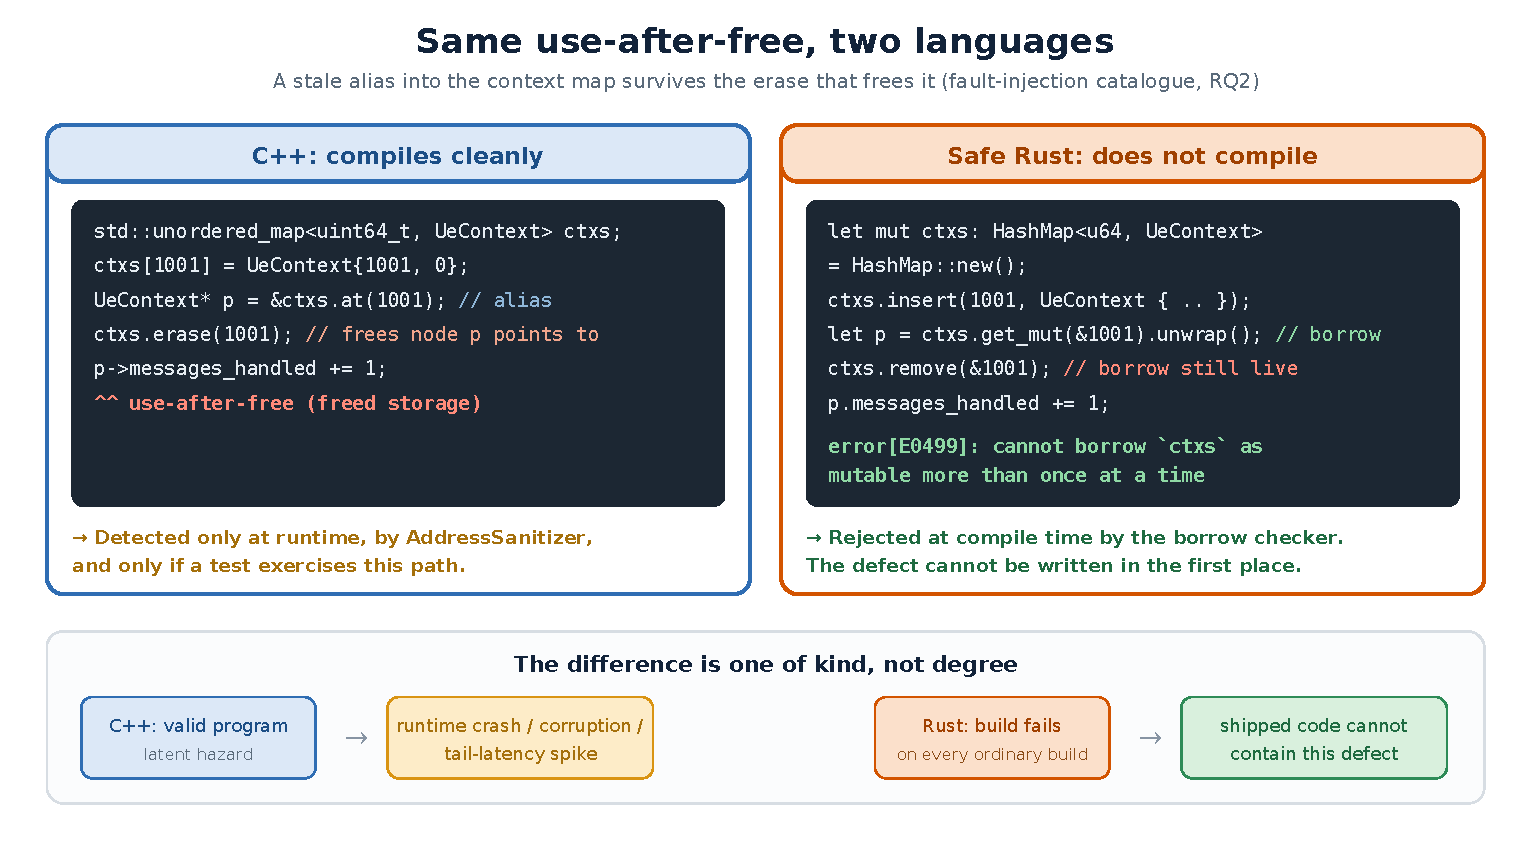
\includegraphics[width=\linewidth]{diagrams/pdf/08_borrow_checker_uaf.pdf}
\caption[The same use-after-free in C++ and in safe Rust]{The same use-after-free defect in C++ and in safe Rust. The stale alias into the
context map survives the \texttt{erase}/\texttt{remove} that frees it: in C++ this compiles and
is caught only at runtime (and only under AddressSanitizer, on a path a test exercises), whereas
in safe Rust the borrow checker rejects it at compile time (\texttt{E0499}), so the defect
cannot be written at all. The difference is one of kind, not degree.\label{fig:borrowuaf}}
\end{figure}

The same discipline extends to concurrency. Rust encodes thread-safety in the type
system through the \texttt{Send} and \texttt{Sync} marker traits: a value may cross a thread
boundary only if its type is \texttt{Send}, and may be shared by reference across threads only
if it is \texttt{Sync}. Sharing a value that permits unsynchronised mutation is therefore a
compile error, not a latent race. This is the property Rust markets as ``fearless concurrency.''
Error handling is likewise explicit: fallible operations return a \texttt{Result} value that
the caller must handle, rather than raising an exception that unwinds through hidden control
flow. Both the cost and the control flow of the failure path therefore stay visible, which is
an advantage in latency-sensitive code where surprises in the tail are what matter.

Rust is not the only memory-safe language, and the reason the comparison here is drawn against
C++ rather than against a managed runtime belongs with this model. Java, C\# and Go achieve
memory safety through a runtime and garbage collection, which is an excellent trade for much
software and a poor one for a tail-latency-critical control plane: collection pauses are a
recognised source of tail latency in large systems~\cite{dean2013tail}, and a managed runtime
cedes the control over memory layout and scheduling this domain relies on. C, at the other
extreme, is as memory-unsafe as C++ while offering fewer abstractions for building large
systems. Rust is the first widely supported language to combine compile-time memory and thread
safety with the absence of a garbage collector and throughput and memory use alongside C and
C++~\cite{balasubramanian2017rust,jung2021safe,bugden2022rust}. That is why managed languages
are out of scope and why the meaningful comparison for RAN control-plane software is C++ against
Rust.

Table~\ref{tab:langmodel} sets the two languages' mechanisms side by side. The distinction it
is built around is not which hazards each language names, since both name much the same ones,
but \emph{when} and \emph{by what} each is ruled out, and the last two rows mark where the
answer stops being ``by the compiler'' for either of them.

\begin{table}
\centering
\small
\caption[How each language enforces the properties measured here]{How each language enforces the properties this thesis measures. The rows above the
rule are the ones on which the two differ in kind rather than in degree: a compiler that
rejects a program rules the defect out of every execution of it, whereas a sanitiser rules it
out only of the executions an instrumented test happens to take. The rows below the rule are
the boundary developed in Chapter~\ref{chapter:context} and measured in
Chapter~\ref{chapter:eval}, where neither language offers a static
guarantee.\label{tab:langmodel}}
\renewcommand{\arraystretch}{1.2}
\begin{tabular}{@{}R{0.20\linewidth} R{0.36\linewidth} R{0.36\linewidth}@{}}
\hline\hline
Concern & Modern C++ & Rust \\
\hline
Object lifetime & RAII and smart pointers, applied by convention. A raw pointer or reference may outlive its referent & Ownership: each value has one owner and is dropped exactly once \\
Aliasing & Unrestricted: any number of mutable aliases may coexist & Borrowing: either one mutable reference or many shared ones, never both \\
Bounds & Unchecked on \texttt{operator[]}, checked only through \texttt{at()} & Checked by default, elided where the index can be proved in range \\
Thread safety & Not expressed in the type system: sharing a mutable object across threads compiles & \texttt{Send} and \texttt{Sync} marker traits. Unsynchronised sharing is a type error \\
Error signalling & Exceptions or error codes: the failure path can be invisible at the call site & \texttt{Result} values the caller must handle. The failure path is explicit \\
Escape hatch & The whole language & \texttt{unsafe} blocks, delimited and mechanically countable \\
Stage of detection & Run time, under the right sanitiser, on a path a test exercises & Compile time, on every ordinary build, whatever the test coverage \\
\hline
Lock-acquisition order & Not checked & Not checked \\
Atomicity of a composed operation & Not checked & Not checked \\
\hline
\end{tabular}
\end{table}

\section{Concurrency models for control-plane software}
How concurrency is structured shapes both correctness and tail latency. The dominant model is
\emph{shared-memory} concurrency, in which threads mutate common state guarded by mutexes and
atomics. It is flexible but is the source of races, deadlocks, lock contention, and priority
inversion, and its worst-case timing is hard to reason about. The alternative is
\emph{message-passing} or \emph{shared-nothing} concurrency, in which state is partitioned so
that each piece is owned by a single thread and all interaction happens through messages, as
in the actor model and in sharded designs. Shared-nothing trades some flexibility for
scalability and far simpler reasoning, and it maps naturally onto per-UE partitioning in a
control plane, where each UE's state is largely independent. The choice is not neutral with
respect to the quantity this thesis measures: thread-per-core structuring has been shown to
change application tail latency in its own right~\cite{enberg2019threadpercore}, which is one
reason the model is held fixed across both implementations rather than left to each language's
idiom. Figure~\ref{fig:concmodels} contrasts the two models and marks what each does to the
hazards catalogued above.

\begin{figure}
\centering
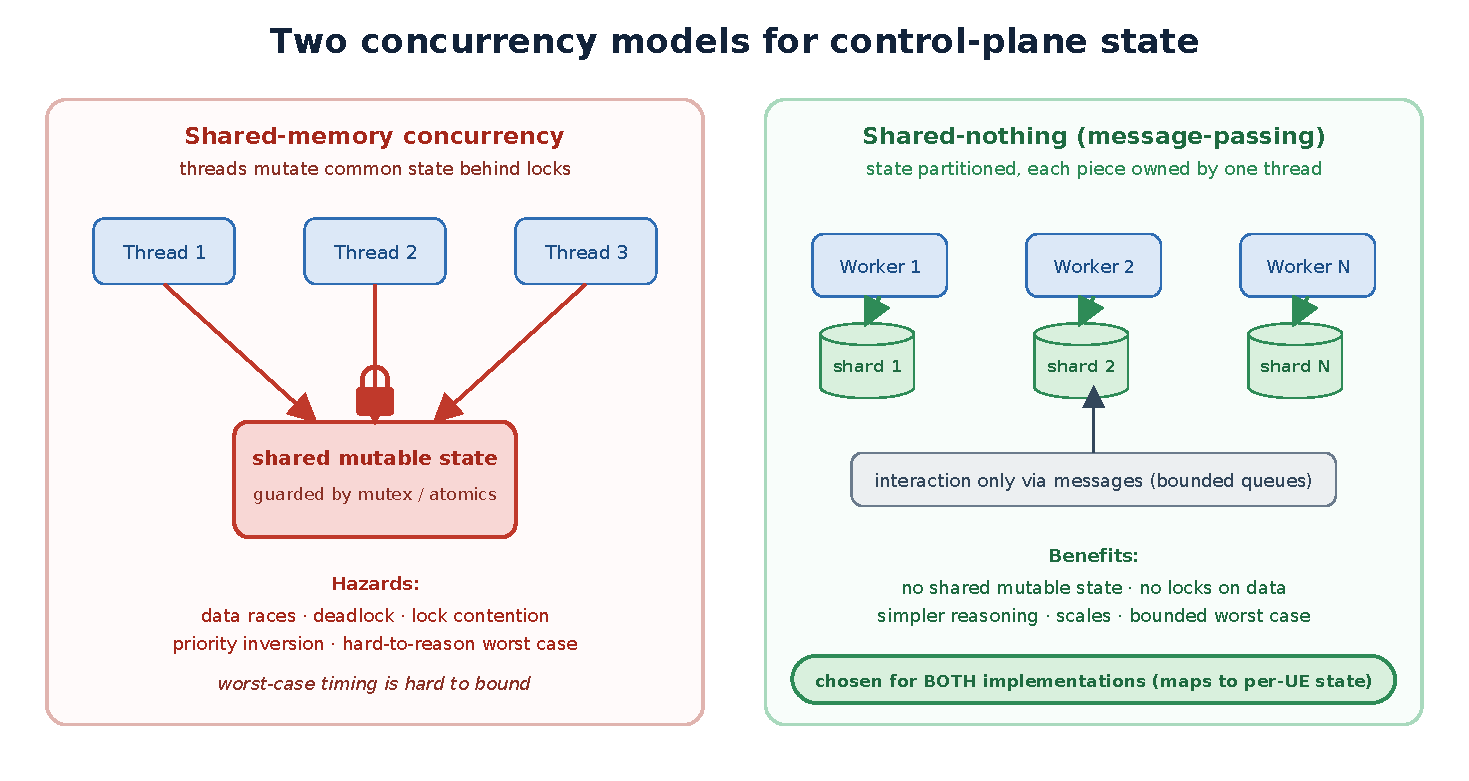
\includegraphics[width=\linewidth]{diagrams/pdf/12_concurrency_models.pdf}
\caption[Two concurrency models for control-plane state]{Two concurrency models for control-plane state. Shared-memory concurrency (left) lets
threads mutate common state behind locks and is the source of data races, deadlock, and lock
contention, with a worst case that is hard to bound. Shared-nothing message-passing (right)
partitions state so each shard is owned by a single worker and all interaction happens through
bounded queues. This eliminates locks on context data and maps naturally onto per-UE
partitioning, and is the model adopted for both implementations.\label{fig:concmodels}}
\end{figure}

A third structure, an asynchronous runtime over a work-stealing scheduler, is idiomatic in both
languages and is deliberately used in neither. Its timing behaviour belongs to the runtime rather
than to the language hosting it: a real-time study of asynchronous Rust finds that one and the
same application meets or misses its deadlines depending on which runtime and thread-priority
mapping it is given, and that the configuration meeting them is not the idiomatic work-stealing
one~\cite{skoudlil2025asyncrust}. Adopting such a runtime would therefore introduce a variable
that this study is built to exclude, and Section~\ref{sec:relatedwork} returns to a comparison in
which it was not excluded.

A second, independent choice is how work is queued between producers and consumers. Unbounded
queues mask overload and let latency and memory grow without limit. \emph{Bounded} queues with
either blocking (backpressure) or shedding bound worst-case memory and make overload visible,
which is essential for predictable tail latency. Lock-free structures can reduce contention
but are notoriously difficult to implement correctly. These considerations directly motivate
the architecture adopted for both implementations in Chapter~\ref{chapter:design}: a
shared-nothing, thread-per-shard design. The UE state is divided into independent slices called
\emph{shards}, and each shard is owned by exactly one worker thread, so no two threads ever
touch the same context. Requests reach a shard through a bounded multi-producer,
single-consumer queue that blocks when full. This model is chosen so that any measured latency
difference reflects the language rather than a divergent concurrency strategy.

\section{Interoperability between C++ and Rust}\label{sec:interop}
Adopting a new language in a large existing system is necessarily incremental: a Rust
component must coexist with, and be callable from, a substantial C++ codebase. The common
denominator for such interoperability is the C application binary interface (ABI). Rust can
expose functions with \texttt{extern "C"} linkage and hand out \emph{opaque handles} to
Rust-owned objects, which C++ then calls through a C header. Tooling automates parts of this,
including \texttt{bindgen} (generating Rust bindings from C headers), \texttt{cbindgen}
(generating C headers from Rust), and the \texttt{cxx} crate (a safer bidirectional bridge).
Interoperability is not free: crossing the boundary steps outside the checked language, so the
seam must contain \texttt{unsafe} code; passing anything beyond simple values requires
marshalling; and the shape of the foreign interface has to be designed deliberately. The size
of that seam, how much \texttt{unsafe} it concentrates, and the per-call crossing cost are
exactly the quantities measured for RQ4 in Chapter~\ref{chapter:eval}.

A distinction has to be drawn at this point, because it bounds what any of those measurements
can establish. Concentrating \texttt{unsafe} in the seam is a statement about what the compiler
checks, not about what can happen at run time. Once a Rust component is linked into a C++ host
they share one address space, and a defect on the C++ side can corrupt Rust-owned data
irrespective of how much of the Rust side the borrow checker verified. This has been
demonstrated experimentally, and the proposed remedies rely on hardware or runtime isolation of
the two heaps rather than on the discipline of the
interface~\cite{rivera2021galeed,kirth2022pkrusafe}. The defect classes arising specifically at
Rust/C boundaries have been catalogued separately from those of either
language~\cite{li2022crosslang}, and the binding generators themselves are known to carry
bugs~\cite{cai2026interop}. The consequence for this thesis is stated once here and honoured
throughout: an \texttt{unsafe}-free core means the core's own defects are ruled out at compile
time, and it does not mean the core is protected from its host.

\section{Research gap}\label{sec:gap}
The preceding sections establish three things. First, the RAN control plane is a
soft-to-firm real-time, highly concurrent, latency-critical domain in which tail behaviour
under overload, not average throughput, governs the quality experienced by the network.
Second, C++ supplies the control and performance this domain demands but leaves whole classes
of memory and concurrency defects to best-effort, after-the-fact detection. Third, Rust
promises to prevent those classes at compile time at no runtime cost, with a credible
incremental adoption path through C-ABI interoperability.

The domain is not unstudied, and the volume of prior work is easy to underestimate because
almost none of it is indexed. At least five vendor-hosted master's theses, all carried out at
Ericsson, have compared candidate languages for RAN and telecom software: one weighs runtime
cost against development efficiency across C++, Rust, and Go~\cite{karlback2021ran}; one asks
whether Rust could replace C in RAN node management~\cite{olsson2023ranmgmt}; one builds a
thread-per-core packet processor on asynchronous Rust and measures it against the DPDK
application it mirrors~\cite{olsson2023asyncpackets}; one measures median and 99th-percentile
latency for control-plane procedures across five asynchronous programming
frameworks~\cite{arvidsson2025async}; and one builds matched C++ and Rust implementations of an
ASN.1 decompiler and compares them statistically~\cite{emberg2023asn1}. All five are directly
relevant, and two report differences unfavourable to Rust.

Three of them vary the language together with the runtime and the concurrency model, so a
measured difference cannot be attributed to the language rather than to the framework built on
it~\cite{karlback2021ran,olsson2023asyncpackets,arvidsson2025async}. The effect sizes reach a
factor of five, which is an indication of how much of the measurement the runtime owns. The
remaining two hold the design closer to fixed but report execution time and peak memory rather
than tail behaviour under rising load~\cite{olsson2023ranmgmt,emberg2023asn1}, and the closest
of them, Emberg and Wadsten, measures a stateless transformation rather than a stateful,
concurrent subsystem. Figure~\ref{fig:gapmap} sets the neighbouring studies against the
properties a controlled answer would require, and the pattern it shows is that each holds some
of them and none holds all.

The concentration of that evidence is itself part of the gap. All five studies come from one
vendor, and their conclusions have never been tested against another organisation's software,
targets or conventions, so what is known about this question is what one company's frameworks
report about it. The published record on the other side is emptier: there is no study of Rust
among the indexed publications of the vendor hosting this work, and the nearest peer-reviewed
position from that side argues for making memory-error sanitisation practical rather than for
replacing it with a compile-time guarantee~\cite{gjomemo2016mesc}, which is the strategy this
thesis tests against. Section~\ref{sec:relatedwork} compares the five with this study directly.

\begin{figure}
\centering
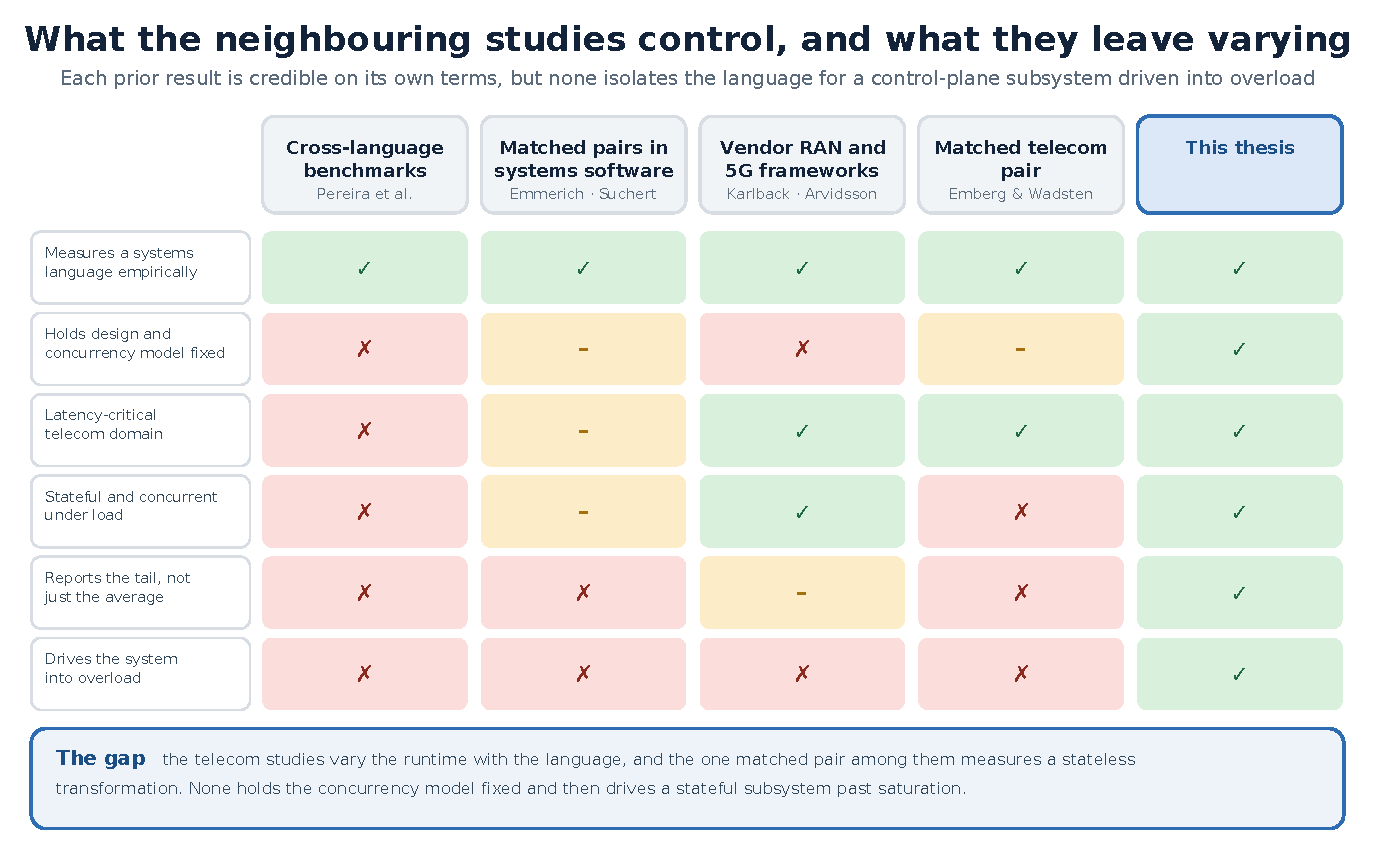
\includegraphics[width=\linewidth]{diagrams/pdf/29_research_gap.pdf}
\caption[What the neighbouring studies control, and what they leave varying]{What the neighbouring studies control, and what they leave varying. Each row is a
property that a controlled answer to the research questions would need. Each column is a study.
The general cross-language comparisons measure the right kind of object but the wrong regime,
reporting averages on general-purpose workloads. Matched pairs in systems software hold the
design fixed, but outside this domain and below saturation. The vendor RAN and 5G framework
studies reach the right domain, and one of them reports the tail, but in all of them the
language varies together with the runtime and the concurrency model. The one matched telecom
pair, Emberg and Wadsten, controls the design but measures a stateless transformation. Holding
the design and the concurrency model fixed for a stateful, concurrent subsystem and then driving
it past saturation is what this thesis adds. The contribution is the control, not a new
measurement technique.\label{fig:gapmap}}
\end{figure}

What is therefore missing from the literature
is \emph{direct, controlled} evidence for a representative control-plane subsystem: whether
Rust actually holds its tail latency and predictability under overload against modern C++
\emph{when the concurrency model, algorithms, and data structures are held fixed},
exactly which defect classes it eliminates and at what stage the remainder are caught, what
its safety model costs in throughput and resources, and what incremental adoption costs in
practice. Closing this gap is the purpose of the four research questions. The next chapter
grounds them in the specific subsystem, defect classes, and timing properties at stake, and
Chapter~\ref{chapter:methodology} sets out the methodology by which they are pursued.

\chapter{Problem Context: UE Context Management and Predictability\label{chapter:context}}
\chaptermark{Problem Context}

\section{The UE Context Management subsystem}
The subsystem under study is a UE Context Management service. It is modelled on a real Nokia
gNB-CU-CP service domain that owns the UE context lifecycle, RRC procedure
execution~\cite{3gpp38331}, and mobility/handover. Those are the very functions the 3GPP
architecture assigns to the control-plane part of a disaggregated gNB: the CU-CP hosts the RRC
and the control-plane part of PDCP and manages the UE context, delegating user-plane bearer
handling to the CU-UP over the E1 interface~\cite{3gpp38401,3gpp38300,3gpp38463}.

It is a good representative on four counts. It is core RAN L3 functionality, it is performance-
and latency-sensitive, it is inherently stateful and concurrent, and it is self-contained
enough to specify precisely and benchmark fairly. The modelled functionality includes UE
context creation and deletion, state transitions (e.g.\ idle to connected), signalling
message handling, and concurrent context lookup under load.

Figure~\ref{fig:fsm} shows the UE-context lifecycle state machine that both implementations
encode identically. Illegal transitions, for example signalling an \texttt{Idle} context, return
a typed error rather than mutating state. This state machine is exactly what the mixed workload
of Section~\ref{sec:workload} walks each UE through.

\begin{figure}
\centering
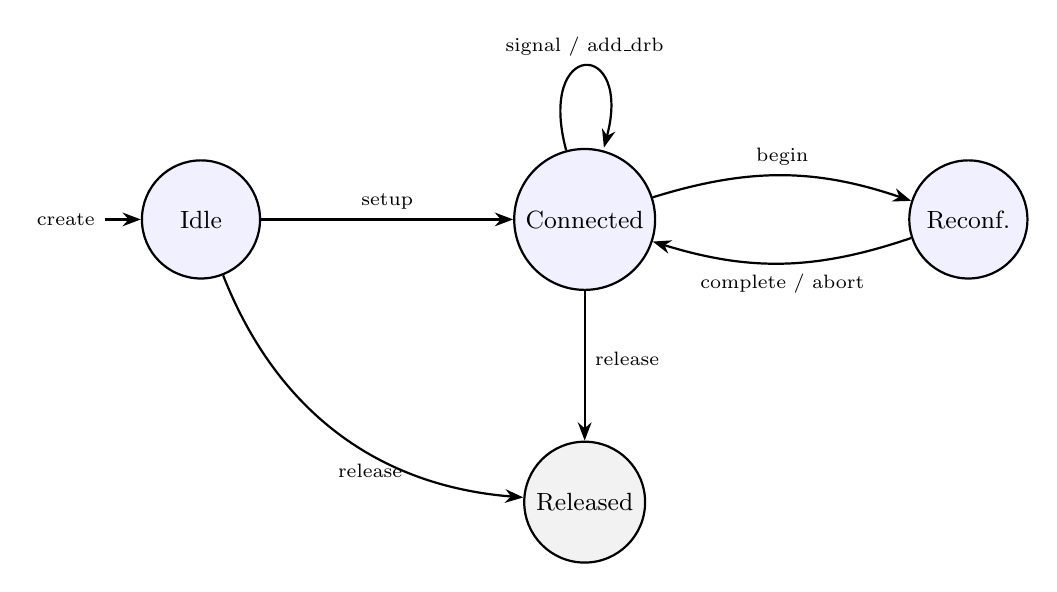
\begin{tikzpicture}[
    ->, >=Stealth, node distance=3.2cm, font=\small,
    every state/.style={draw, minimum size=1.5cm, fill=blue!6, thick},
    every edge/.style={draw, thick}
  ]
  \node[state, initial, initial text=\scriptsize create] (idle) {Idle};
  \node[state, right=of idle] (conn) {Connected};
  \node[state, right=of conn] (reconf) {Reconf.};
  \node[state, below=1.9cm of conn, fill=gray!10] (rel) {Released};

  \path (idle)  edge node[above,font=\scriptsize]{setup} (conn)
        (conn)  edge[bend left=18] node[above,font=\scriptsize]{begin} (reconf)
        (reconf) edge[bend left=18] node[below,font=\scriptsize]{complete / abort} (conn)
        (conn)  edge node[right,font=\scriptsize,pos=0.45]{release} (rel)
        (idle)  edge[bend right=32] node[below,font=\scriptsize,pos=0.6]{release} (rel);
  \path (conn) edge[loop above] node[font=\scriptsize]{signal / add\_drb} (conn);
\end{tikzpicture}
\caption[UE-context lifecycle state machine]{UE-context lifecycle state machine. \texttt{create} allocates a context in
\texttt{Idle}; \texttt{setup} connects it; \texttt{signal} and \texttt{add\_drb} are handled
in place while \texttt{Connected}; a reconfiguration/handover moves through
\texttt{Reconfiguring} and back on \texttt{complete} or \texttt{abort}; \texttt{release}
tears the context down. Operations invalid for the current state return an \texttt{OpError}
instead of changing state.\label{fig:fsm}}
\end{figure}

\paragraph{Representativeness and tractability.}
Two properties make UECM a good study object for a language comparison. It is
\emph{representative}: per-UE mutable state, a strict operation lifecycle, high inter-UE
concurrency, and the hard latency and reliability targets the 5G system places on control-plane
procedures~\cite{3gpp38913,3gpp22261} are exactly the properties that make production
RAN control-plane code difficult, so conclusions about how a language handles them transfer to
the broader class of stateful, concurrent control-plane services. It is also \emph{tractable}:
the subsystem is small enough to specify precisely, implement faithfully in two languages, and
reason about in full, which is what makes a controlled, parity-tested comparison possible at
all. A larger or less well-bounded subsystem would improve external validity at the cost of the
internal validity on which a fair language comparison depends. UECM is chosen as the point that
keeps both within reach.

\paragraph{Operation set.}
The interface exercised by the study is deliberately small and lifecycle-oriented: create and
release a context; set up a connection (\texttt{Idle}$\rightarrow$\texttt{Connected}); handle an
in-session signalling message; add a data radio bearer; begin, complete, or abort a
reconfiguration/handover; and look up a context's state under concurrent load. Every operation is
defined for every state of the machine in Figure~\ref{fig:fsm}: an operation that is illegal in
the current state returns a typed error and leaves the context unchanged, rather than throwing
or corrupting state. This closed, well-typed operation set is what lets the same test vectors
and the same workload drive both implementations along identical paths
(Section~\ref{sec:parity}).

\section{Memory-safety and concurrency defect classes}
The defects that affect C++ control-plane code of this kind fall into two families. The
\emph{memory-safety} family concerns the lifetime and bounds of objects: a \emph{use-after-free}
accesses storage that has already been released, a \emph{double-free} releases the same storage
twice, and a \emph{buffer overflow} reads or writes past the end of an allocation. The
\emph{concurrency} family concerns unsynchronised or ill-ordered access from multiple threads: a
\emph{data race} is a pair of unsynchronised accesses to the same location of which at least one
is a write, a \emph{deadlock} is a cyclic wait for locks, and \emph{iterator invalidation} is
the use of an iterator or reference into a container after a mutation has moved or freed the
underlying storage. What these share is that they are all \emph{silent} in C++: each is accepted
by the compiler and, on the paths ordinary tests happen to exercise, may appear to work,
surfacing only later as corruption, a crash, or an unpredictable latency spike. These are the
same memory-corruption classes that decades of security research have struggled to contain in C
and C++~\cite{szekeres2013sok}.

Each class has a natural incarnation in UE Context Management, which is why the subsystem is a
good vehicle for studying them:

\begin{itemize}
  \item \textbf{Use-after-free.} A signalling message holds a raw pointer or reference to a UE
        context that a concurrent \texttt{release} has already erased from the context map. The
        in-flight handler then dereferences freed storage.
  \item \textbf{Double-free.} A release path runs twice for the same UE, for example because a
        retransmitted release is not made idempotent, freeing the context's owned resources a
        second time.
  \item \textbf{Iterator invalidation.} Code iterates a context's data-radio-bearer list while
        adding or removing a bearer, so the iterator refers into storage the container has since
        reallocated.
  \item \textbf{Data race.} Two workers update the same context field, an activity counter or a
        state flag, without synchronisation, so the accesses race.
  \item \textbf{Unguarded shared mutation.} A context is shared by reference across threads and
        mutated without a lock or other discipline, a race whose root cause is the absence of any
        ownership rule for the shared state.
\end{itemize}

These five classes lie squarely within the guarantees Rust claims to provide, which makes them
the natural test of whether that claim holds. Testing only them, however, would build the
expected answer into the choice of test cases, so five further classes are carried into the
study for the opposite reason, because there is good reason to expect that safe Rust does
\emph{not} prevent them:

\begin{itemize}
  \item \textbf{Lock-order deadlock.} A handover locks the source UE context and then the
        target while a concurrent handover in the opposite direction locks target then source,
        and the two wait for each other indefinitely. Nothing about object lifetimes or
        aliasing is violated. The fault is in the order of acquisition.
  \item \textbf{Lost update.} Two workers increment a context's activity counter through a
        read-modify-write split across two separate critical sections. Every individual access
        is correctly synchronised, so this is a \emph{race condition} rather than a
        \emph{data race}: the atomicity violation lives in the composition of the operations,
        not in the memory accesses themselves, and it corrupts a value silently instead of
        crashing.
  \item \textbf{Leak through a reference cycle.} A context and the peer it is being handed
        over to hold owning references to each other, so neither reference count reaches zero
        and neither is ever destroyed. Reference counting cannot collect a cycle in either
        language, and leaking is safe in Rust by explicit design. This is the cleanest
        statement of a boundary in the catalogue, because both languages fail identically.
  \item \textbf{Integer overflow in a release build.} A bearer's TEID stride computation
        exceeds the width of its type. In C++ signed overflow is \emph{undefined}, so the
        program has no meaning. In Rust it is \emph{defined} to wrap, because the
        \texttt{opt-level~=~2} profile this study compares leaves \texttt{overflow-checks}
        off, so the program has a meaning and the meaning is wrong. The pattern is not
        hypothetical: CVE-2026-64467 in \texttt{rust\_binder} is a stride error of this shape.
  \item \textbf{Worker failure blast radius.} One shard worker fails part-way through a
        procedure. The concurrency model of Section~\ref{sec:concurrency} makes a shard
        a failure domain by construction, and neither language's type system enforces that it
        behaves as one: in C++ an exception escaping the thread callable terminates the whole
        process, and in Rust the panic is confined to its thread but poisons the state it held,
        so the damage propagates along the data instead. Directly relevant to a carrier-grade
        availability argument, and addressed by nothing in either type system.
\end{itemize}

Together these ten form the catalogue injected in Chapter~\ref{chapter:eval}, and the split
between the two groups is what lets the study report a boundary rather than a verdict. Buffer
overflow is described above for completeness but is not injected, because neither
implementation performs raw pointer arithmetic on the context store, so an injected instance
would be an artificial construct and not a plausible bug in this subsystem.
Table~\ref{tab:defectmap} collects the catalogue with the outcome expected of each case
\emph{before} the study was run, which is the form in which the runner records it: an
expectation written down in advance can be violated in either direction and reported as a
discrepancy, whereas one formed after the fact cannot.

\begin{table}
\centering
\small
\caption[The injected catalogue and its incarnations in UECM]{The injected defect catalogue: each class in the form it would plausibly take in UE
Context Management, and the outcome recorded for it in advance of the study. The last column
is a prediction rather than a result. Table~\ref{tab:taxonomy} reports what was measured, and
the fault runner flags a mismatch in either direction instead of absorbing it into the
conclusion. Buffer overflow is listed for completeness and not injected: neither
implementation does pointer arithmetic on the context store.\label{tab:defectmap}}
\footnotesize
\renewcommand{\arraystretch}{0.95}
\begin{tabular}{@{}R{0.19\linewidth} R{0.40\linewidth} R{0.14\linewidth} R{0.16\linewidth}@{}}
\hline\hline
Defect class & Incarnation in UE Context Management & How it fails & Expected in safe Rust \\
\hline
\multicolumn{4}{@{}l}{\emph{Memory-safety family: object lifetime and bounds}} \\
Use-after-free & An in-flight signalling handler dereferences a context that a concurrent \texttt{release} has already erased from the map & Corruption or crash & Prevented \\
Double-free & A retransmitted release is not made idempotent, so the release path frees the context's resources a second time & Corruption or crash & Prevented \\
Buffer overflow & No plausible incarnation here: the context store is reached only through container APIs & n/a & Not injected \\
\hline
\multicolumn{4}{@{}l}{\emph{Concurrency family: unsynchronised or ill-ordered access}} \\
Iterator invalidation & A bearer is added while the context's data-radio-bearer list is being iterated & Corruption or crash & Prevented \\
Data race & Two workers update the same context field, a counter or a state flag, without synchronisation & Torn or lost value & Prevented \\
Unguarded shared mutation & A context is shared across threads and mutated with no ownership rule governing it & Torn or lost value & Prevented \\
\hline
\multicolumn{4}{@{}l}{\emph{Boundary group: included because safe Rust is expected \emph{not} to prevent them}} \\
Lock-order deadlock & Opposing handovers lock source-then-target and target-then-source & Hang & Not prevented \\
Lost update & A counter's read-modify-write is split across two critical sections, so each access is synchronised but their composition is not atomic & Silently wrong value & Not prevented \\
Reference-cycle leak & A context and its handover peer hold owning references to each other, so neither reference count reaches zero & Unbounded growth & Not prevented \\
Integer overflow (release build) & A bearer's TEID stride computation exceeds the width of its type & Silently wrong value & Not prevented \\
Worker-failure blast radius & One shard worker fails part-way through a procedure while holding shard state & Outage beyond one shard & Not prevented \\
\hline
\end{tabular}
\end{table}

\section{Tail latency and predictability in RAN}
Section~\ref{sec:predictability} set out why the tail rather than the mean governs a
latency-critical system, and what measuring it correctly demands. What that section left
general, this one makes specific, because two properties of the RAN setting are what turn a
methodological preference into the governing metric.

The first is \emph{fan-out}: a single user-visible action, a call setup or a handover,
decomposes into many dependent control-plane operations, and because the slowest of them gates
completion, a latency that is rare per operation becomes common per
procedure~\cite{dean2013tail}. The second is \emph{scale}: a busy site drives thousands of such
procedures per second across millions of connected devices, so a tail event occurring once in a
thousand operations is not an edge case but a routine occurrence somewhere in the fleet at
every instant. Taken together, the p99.9 of a single UE Context Management operation is not a
curiosity at the margin of a distribution. It is a rate of degraded procedures the network
sustains continuously.

The scale at which those percentiles matter is not hypothetical. A measurement study of a
disaggregated 5G RAN times the CU-CP-to-DU UE Context Setup procedure over F1-C, and the
CU-CP-to-CU-UP bearer context setup over E1, under different interface-protection schemes, and
finds the choice worth hundreds of microseconds: on F1-C, IPsec adds on the order of
$120\,\mu$s on average to UE context setup, against roughly $430\,\mu$s for
DTLS~\cite{michaelides2026ranlatency}. Overheads of that size are treated as consequential for
precisely the procedure family this thesis reimplements, which places these operations in a
regime where tens of microseconds are an engineering quantity rather than noise.

The study therefore characterises the full latency distribution, focusing on the high
percentiles (p99 and p99.9) and the maximum, and on how these degrade as offered
load approaches and then exceeds saturation (Chapter~\ref{chapter:eval}). Stopping at nominal
load would miss the regime that decides service quality, since queueing delay grows
super-linearly near capacity. It is also the regime in which a difference between two
implementations of one design, if there is one, has room to become visible.

\begin{figure}
\centering
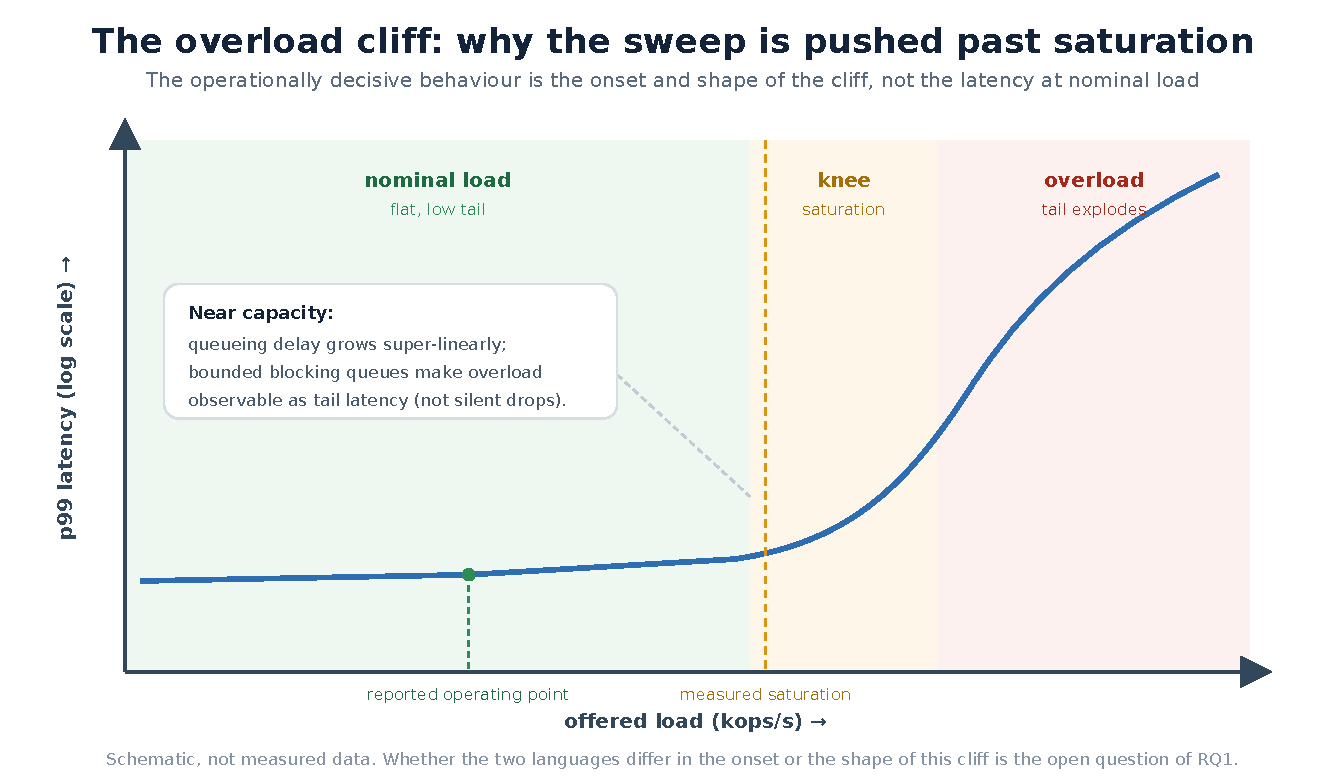
\includegraphics[width=0.9\linewidth]{diagrams/pdf/15_overload_cliff.pdf}
\caption[The overload cliff]{The overload cliff. Tail latency stays low and flat while offered load is below
service capacity, then climbs steeply once the system is driven past saturation and requests
queue behind the bounded, blocking queues. The operationally decisive behaviour is the onset and
shape of this cliff, which is why the load sweep is pushed beyond the saturation point rather
than stopping at nominal load. The figure is a schematic of the phenomenon and not a plot of
this study's data: whether the two languages differ in where the cliff begins or how steeply it
rises is exactly what RQ1 asks, and Section~\ref{sec:perfresults} reports that the development
host cannot resolve it.\label{fig:cliff}}
\end{figure}

\chapter{Research Methodology\label{chapter:methodology}}

The previous chapter set out what the study must achieve. This one sets out how. It states
the overall research strategy, the method chosen for each research question and why it is
appropriate, the controls that make a language comparison fair, the statistical treatment of
the measurements, and the reproducibility and ethical commitments under which the work is
carried out.

\section{Research approach}
The thesis follows an empirical, experimental research approach with a constructive
(design-science) element. A software artifact, two functionally equivalent implementations
of the subsystem together with a benchmarking framework, is built against a single frozen
specification and then evaluated under controlled experiments. Evidence is triangulated from
three complementary methods: quantitative performance measurement under a swept load
(addressing RQ1 and RQ3), a controlled fault-injection study of defect detection (RQ2), and
a qualitative-plus-quantitative FFI migration case study (RQ4). Fairness is treated as a
first-class concern: because the goal is to isolate language effects, the study fixes the
specification, algorithms, concurrency model, allocator, and build settings across both
implementations, and reports variance over repeated runs.

The gap this design addresses (Section~\ref{sec:gap}) is only as good as the search that looked
for it, so the search is stated rather than assumed. Candidate literature was gathered from the
ACM Digital Library, IEEE Xplore, USENIX, and Google Scholar using combinations of the terms
\emph{Rust}, \emph{C++}, \emph{memory safety}, \emph{tail latency}, \emph{systems programming},
\emph{performance comparison}, and \emph{RAN} / \emph{5G control plane}, restricted to
peer-reviewed venues except where an industry or government report is itself the object of study
(the memory-safety mandates and vendor vulnerability statistics). The result set was extended by
backward and forward citation chaining from the core Rust-safety papers, and filtered to work
that either measures a systems language empirically, formalises Rust's guarantees, or reports
adoption experience. The domain literature (3GPP specifications and the O-RAN survey) was added
separately to fix the architectural context.

Those sources alone would have missed the closest prior work, which is why two more were added.
The vendor-hosted theses that come nearest to this study (Section~\ref{sec:relatedwork}) appear
in none of the citation databases: not in Crossref, OpenAlex, DBLP, or Semantic Scholar. Neither
forward nor backward chaining can reach them, because nothing indexed cites them and their own
reference lists are not deposited. They were found instead by searching the institutional
repositories directly, DiVA for the Nordic universities and Finna for the Finnish ones. The same
two searches establish an absence on the other side. Finna, which federates the Finnish university
repositories, returns no thesis on Rust in a radio-access or telecom context, and an author-
affiliation search of Nokia's indexed publications in OpenAlex returns none either: its entities
hold on the order of thirty thousand indexed works, several hundred of which concern the radio
access network, and one mentions Rust, in an unrelated preprint on trusted-execution monitoring.
The entire domain-specific literature on the language question is therefore Swedish and
Ericsson-hosted, and its transferability is untested rather than established. Two practical notes
belong with the protocol, since both distort a naive search. Free-text queries for
\emph{Rust} in the general indexes rank plant pathology and corrosion chemistry above the
programming language, so field-restricted or discipline-restricted queries are necessary; and
the theses are grey literature, so they are cited here as evidence of what has been attempted
and found, not as peer-reviewed results.

The search returned no study, indexed or grey, that measures the tail-latency behaviour of a
Rust and a C++ implementation of the same stateful, concurrent control-plane subsystem under
overload.

Table~\ref{tab:design} maps each research question to the method, artifact, data, and metric
used to answer it, making the chain from question to evidence explicit and traceable. The chain
continues in one place for all four: every question is judged in Section~\ref{sec:rqdiscussion}
and its hypothesis disposed of in Section~\ref{sec:hypotheses}. RQ1 and RQ3 share H1, which was
worded to cover performance equivalence in both its latency and its resource sense, and
Section~\ref{sec:hypotheses} finds that wording to be the hypothesis's main weakness. RQ2 and RQ4
are environment-insensitive. RQ1 and RQ3 depend on the measurement host and are reported against
what it can carry (Section~\ref{sec:testbed}).

\begin{table}
\centering
\caption[Research design: how each research question is answered]{Research design: how each research question is answered. Every question is tied to a
concrete method, a published artifact, the data it produces, and the metric on which the
conclusion rests. RQ1 and RQ3 carry two methods rather than one: the sweep measures the
round-trip a deployment would experience, and the component decomposition measures the part of
it the language is responsible for. Section~\ref{sec:methodperf} states why one cannot stand in
for the other. RQ1 and RQ3 are tested against H1, RQ2 against H2, and RQ4 against
H3.\label{tab:design}}
\renewcommand{\arraystretch}{1.25}
\begin{tabular}{@{}p{0.06\linewidth} p{0.24\linewidth} p{0.24\linewidth} p{0.32\linewidth}@{}}
\hline\hline
RQ & Method & Artifact / data & Primary metric \\
\hline
RQ1 & Load sweep to overload, interleaved repeats & Benchmark harness, latency histograms &
median, p99/p99.9 tail latency, and maximum vs.\ offered load \\
RQ3 & Same sweep, resource capture & \texttt{getrusage} samples per run &
peak RSS, CPU utilisation, throughput \\
RQ1, RQ3 & Component decomposition: the core called directly, then through the service &
Matched microbenchmark pair, interleaved repeats &
per-operation cost split into the operation and the cross-thread handoff \\
RQ2 & Controlled fault injection & Defect catalogue, ASan/TSan and \texttt{rustc} logs &
defect-class taxonomy (compile-time / runtime / undetected) \\
RQ4 & FFI migration prototype & C++ host $+$ Rust C-ABI seam &
seam size, \texttt{unsafe} scope, per-call interop cost \\
\hline
\end{tabular}
\end{table}

\section{A constructive, comparative experiment}
The four research questions are causal and comparative: each asks how an outcome (tail
latency, prevented defects, resource use, or migration cost) depends on a single independent
variable, the implementation language. Answering such questions credibly requires that the
language be the \emph{only} systematic difference between the two objects under test. This
rules out the most common form of language comparison in the literature, in which two
independently written programs, or two unrelated projects, are measured and their differences
attributed to the language. Such comparisons confound the language with the design, the
libraries, and the intent and skill of their authors. The thesis therefore adopts a
constructive (design-science) strategy: instead of locating two pre-existing systems, it
\emph{builds} the object of study as a matched pair of implementations derived from one frozen
specification, so that the comparison is between two encodings of the same design rather than
between two designs. The artifact, the specification, the two implementations, and the
benchmarking harness, is thus simultaneously the contribution of the thesis and the instrument
through which it is measured.

The experiment is empirical and quantitative where the questions admit numbers (RQ1, RQ3, and
the per-call cost of RQ4) and systematic-but-qualitative where they do not (the
kind-of-guarantee distinction in RQ2 and the API-design effort in RQ4). Evidence is
deliberately triangulated across three complementary methods rather than resting on a single
campaign, so that a weakness in any one method, for example the environment sensitivity of
tail-latency measurement, does not undermine the conclusions as a whole.

\section{Methods for the four research questions}
Table~\ref{tab:design} pairs each question with a method. This section states what each method
does and why it is appropriate.

\subsection{Performance measurement under a load sweep (RQ1, RQ3)}\label{sec:methodperf}
RQ1 and RQ3 are answered by driving both implementations with one deterministic synthetic
workload across a sweep of offered load, from light load through saturation and into overload,
and recording latency and resource use at each level. Two design decisions make the
measurement sound. First, the load generator follows an \emph{open-loop} schedule with a fixed
intended send time per request, and latency is measured against that intended time rather than
against the moment the request is actually admitted. This is what corrects for coordinated
omission in the sense defined in Chapter~\ref{chapter:background}. Second, the sweep is pushed
past saturation deliberately:
the operationally decisive behaviour of a control plane is not its latency at nominal load but
the onset and shape of the overload cliff, and that is visible only once offered load exceeds
service capacity. Latency is captured in high-dynamic-range histograms configured identically
on both sides, and resource use (peak resident set size, CPU utilisation, throughput) is
sampled through the operating system, so that the same measurement apparatus is applied to both
languages.

\paragraph{Measuring the component as well as the round-trip.}
A sweep of this kind measures a round-trip, and a round-trip bundles two costs of quite
different character. One is the operation the language executes inside a single thread: a hash
lookup, a state-machine guard, and a field update, all of it code the compiler generated. The
other is the cross-thread submit-and-complete handoff around it: an enqueue, a futex wake, a
context switch, and a completion, none of it language-specific. Only the first can plausibly
differ between C++ and Rust, and no end-to-end measurement can separate them. The method
therefore operates at two levels. The single-threaded operation processor is called directly,
with no queue in the path, and the same operation is then called through the full threaded
service. The difference between the two is the handoff. Both are batch means over a long loop
and not per-call medians, deliberately: a clock read costs tens of nanoseconds, the same
order as the operation itself, so per-call timestamps would measure the instrument rather than
the code. The two languages are interleaved across repeats and compared with the same exact
paired test as the sweep, so the two levels differ in what they measure, not in how they
are analysed.

Reporting both is what lets the study separate two questions that the research questions as
originally worded did not distinguish: what a deployment of this shape would experience, which
is the round-trip, and what the language is doing, which is the component.
Section~\ref{sec:budget} finds the two to be more than two orders of magnitude apart, so the
distinction is not a refinement but the difference between an interpretable result and an
uninterpretable one. This second level was added after a first pass of the campaign rather than
designed in from the start, and Section~\ref{sec:threats} records that revision instead of
presenting the design as though it had always been complete.

\paragraph{Isolating the contended synchronisation primitives.}
The overload comparison of Section~\ref{sec:overload} attributes its gap to the bounded blocking
queue and the one-shot completion handle, the two forced-idiom entries where the standard libraries
diverge. A third matched microbenchmark isolates those primitives alone: \ContentionProducers{}
producer threads hammer one queue of capacity $1\,024$ while a single consumer drains it, with no
\texttt{ShardCore} work in the path. C++ uses the hand-written \texttt{BoundedQueue} and
\texttt{std::promise}/\texttt{std::future}. Rust uses \texttt{sync\_channel} and a fresh
\texttt{mpsc::channel()} per request. The benchmark is analysed with the same interleaved repeats
and exact paired test as the decomposition above. Section~\ref{sec:contention} reports whether
the isolated primitives reproduce the ordering seen in the full service.

\subsection{Controlled fault injection (RQ2)}\label{sec:methodfaults}
RQ2 asks which defect classes a language prevents, and it cannot be answered by measuring
defect-free code. The absence of a bug in a passing test says nothing about whether the
language would have caught it. The method is therefore adversarial, following the established
practice of software fault injection, in which representative faults are deliberately introduced
to assess how a system behaves in their presence~\cite{natella2016fault}.

A catalogue of representative C++ defects is written \emph{deliberately}, drawn from the classes
that affect this subsystem (Chapter~\ref{chapter:context}). Each is a small self-contained
program flavoured with the domain: a stale pointer into the context map, a double release, a
mutation during iteration, an unsynchronised shared update. Each C++ defect is then built and
run under AddressSanitizer, ThreadSanitizer and UndefinedBehaviorSanitizer, recording which
tool, if any, detects it and at what stage. The analogous construct is written in safe Rust and
compiled, recording the compiler's outcome and, where it compiles, the behaviour of the
resulting program. For the boundary classes, where by construction the compiler has nothing to
say, the Rust side is additionally put to two model checkers, Loom and Shuttle, so that the
``at what stage'' half of RQ2 is answered for them rather than left blank.

One case is repeated rather than run once. Whether ThreadSanitizer reports the lock-order
inversion depends on the schedule, so a single run records whichever outcome the machine
happened to give. The runner therefore executes that case twelve times and reports the rate,
distinguishing an intermittent detection from a reliable one.

\paragraph{Why the C++ side is tooled with sanitisers only.}
No static analyser is run against the C++ catalogue, and that is a decision rather than an
oversight. RQ2 does not ask which tool finds the most defects. It asks at what \emph{stage}, and
with what force, each language rules a defect out, and the taxonomy's three outcomes,
compile-time rejection, runtime detection, and a silent miss, are the categories that question
needs. A static analyser belongs to none of them. It is not the compiler refusing to build a
program, and it is not an observation of an execution that occurred. It is an opt-in pass whose
output is a warning a project can configure away, and which Section~\ref{sec:cpplatency} has
already noted suffers false negatives and cannot reason across a whole program.

What the choice costs is worth stating plainly, because it makes the C++ side of the resulting
taxonomy narrower than the best a C++ project could manage. The memory-safety cases are small
and intra-procedural, which is the shape at which static analysis is strongest, so a
well-configured analyser could plausibly reach some of them. The concurrency cases, whose
manifestation depends on an interleaving, are the shape at which it is weakest. The study
therefore reports the tooling it ran, which is the sanitiser-based practice described in
Section~\ref{sec:cpplatency}, and not a ceiling on what C++ tooling can achieve. One property no
analyser would change is the one the comparison turns on. A warning a build can be
configured to ignore is a different kind of object from a compilation that cannot succeed, and
it is that difference, rather than a count of detected defects, that the method measures.

The comparison is controlled in the same way as the performance one. Because the independent
variable is again only the language while the injected fault is held fixed, the difference in
outcome is attributable to the language's guarantees rather than to the specific bug. That
outcome is one of three: compile-time rejection, runtime detection, or a silent miss. The result
is a taxonomy, not a performance number: the method establishes the \emph{kind} of
protection each language offers.

One design decision determines whether that taxonomy can be trusted. A catalogue drawn only
from classes the language is known to prevent would produce a foregone conclusion: the method
would be capable of confirming the hypothesis but not of disturbing it, and the result would
describe the author's choice of cases as much as the language. The catalogue is therefore
constructed in two groups. The first contains classes that lie inside Rust's stated guarantee.
The second contains classes deliberately chosen from just outside it, where ownership and the
\texttt{Send}/\texttt{Sync} discipline give no protection. Each case carries a recorded
expectation, prevented or not prevented, and the runner reports a violation in either
direction, so an unexpected outcome would surface as a discrepancy instead of being absorbed
into the narrative. What this buys is a boundary rather than a score: the study can state not
only which defect classes the language removes but which comparable ones it leaves in place,
and the second half of that statement is the part a practitioner planning a migration
needs.

\subsection{Foreign-function-interface migration case study (RQ4)}\label{sec:methodffi}
RQ4 concerns the practical cost of adopting Rust inside an existing C++ system, which is an
engineering question as much as a performance one. It is answered by constructing a working
prototype in the realistic direction of migration: an existing C++ host calling a Rust
component across a C application binary interface. Three quantities are then measured on it.
The \emph{size} of the interoperability seam counts its entry points, lines of code, and
dependencies. The \emph{scope} of \texttt{unsafe} records where the checked language is left
and whether the safety-critical core is affected. The \emph{per-call cost} is the price of
crossing the boundary, measured against the same operation invoked natively so that the
comparison isolates what the seam adds rather than what the operation costs. The first two are
structural and are read off the code. The third is a matched pair of microbenchmarks.
This combination of a structural account and a quantitative cost measurement is what lets the
study separate the run-time cost of interoperability from its true cost, which lies in API
design and human learning.

\section{Fairness as a controlled-variable strategy}
Because every research question attributes a difference to the language, the validity of the
whole study depends on holding everything else equal, and fairness is treated as the study's
central experimental control and not as an afterthought. It is enforced at several levels.
The \emph{specification} is frozen before any code is written and fixes the public API, the
state machine, the data structures and their algorithmic strategy, and the sharding and
concurrency model (Section~\ref{sec:fairness}). The \emph{run-time substrate} is equalised by
linking the same memory allocator on both sides and matching build-optimisation levels as
closely as the two toolchains allow. The \emph{workload} is produced by a driver that is
identical in structure across languages and, for a given seed and active-UE population, drives
both implementations through exactly the same sequence of operations, so that any latency
difference reflects how each language executes the same work rather than a difference in what
work is done. Where the two languages genuinely cannot express the same construct, the deviation
is not hidden but recorded in a forced-idiom log so it can be weighed explicitly in the
discussion. What remains uncontrolled, principally single-author skill asymmetry, is
acknowledged as a threat to validity (Chapter~\ref{chapter:discussion}), not claimed to
be eliminated.

Table~\ref{tab:controls} states the strategy variable by variable, and its third column is the
part that matters most. A controlled experiment is credible in proportion to the honesty of
its account of what it failed to control, and three of the rows below record a residual and not
a clean fix: the languages cannot always express the same construct, they do not ship the
same hash-map layout, and one person wrote both implementations. Both escape valves are part of
the design rather than exceptions to it: the forced-idiom log records where the languages cannot
be held identical, and the last row names the one variable left with no control at all.

\begin{table}
\centering
\small
\caption[The controlled-variable strategy]{The controlled-variable strategy: what is held fixed so that the language remains the
only systematic difference, and what each control does not reach. The third column is not a
list of oversights but the study's own account of its limits. Each entry is picked up again as
a threat to validity in Section~\ref{sec:threats}. Only the last row names a variable for
which there is no control at all.\label{tab:controls}}
\footnotesize
\renewcommand{\arraystretch}{1.15}
\begin{tabular}{@{}R{0.16\linewidth} R{0.44\linewidth} R{0.32\linewidth}@{}}
\hline\hline
Variable & How it is held fixed & What the control does not reach \\
\hline
Design & One specification, frozen before any code is written, fixing the public API, the state machine, the data structures and their algorithmic strategy, and the sharding granularity (\S\ref{sec:fairness}) & Where the two languages cannot express the same construct, the divergence is logged, not removed (Table~\ref{tab:idioms}) \\
Concurrency model & Thread-per-shard over bounded blocking MPSC queues on both sides, with no asynchronous runtime on either & Nothing outstanding \\
Hashing & SplitMix64 for shard selection and FNV-1a inside the shard, pinned identically, so neither standard library's default hasher becomes an accidental advantage & The container itself is still each language's own hash map, and the two differ in layout (\S\ref{sec:budget}) \\
Allocator & The same \texttt{jemalloc} linked on both sides, with a system-allocator build kept on each as a control & Nothing outstanding \\
Optimisation & \texttt{-O2} against \texttt{opt-level~=~2} & Nominal parity is not identical code generation \\
Workload & One deterministic driver. For a given seed and active-UE population both implementations execute the same operation sequence, checked by per-kind counts & Synthetic and spec-justified rather than replayed from production traffic \\
Instrumentation & The same HDR histogram algorithm and configuration, the same open-loop schedule, the same repeat and interleaving discipline & Nothing outstanding \\
Behaviour & A language-neutral conformance suite whose canonical transcripts are diffed op for op (\S\ref{sec:parity}) & Parity bounds behaviour, not performance \\
\hline
Author & No control & One person wrote both implementations and is not equally expert in both \\
\hline
\end{tabular}
\end{table}

\section{Statistical treatment of measurements}\label{sec:stats}
Performance measurements are non-deterministic, so single-run numbers are avoided throughout.
Each configuration (language $\times$ allocator $\times$ load level) is measured over many
independent repeats, and the four variants are \emph{interleaved} within each repeat so that
slow drift, thermal effects, and background activity perturb them equally instead of biasing
one. Results are summarised by the median with a nonparametric bootstrap $95\%$ confidence
interval~\cite{efron1993bootstrap} rather than by the mean with a standard deviation, because
latency distributions are
heavy-tailed and skewed and a distribution-free interval on the median makes no normality
assumption. This follows established guidance on statistically rigorous performance evaluation,
which warns that reporting a single number invites conclusions that run-to-run variation does
not support~\cite{georges2007rigorous}. Tail percentiles (p99, p99.9, p99.99) are read from the
HDR histograms, whose logarithmic bucketing retains three significant figures of resolution
across the whole range so that high percentiles are not quantised away. Intervals are reported
in full, not as a symmetric half-width, because a bootstrap interval on the median of a
heavy-tailed sample is markedly asymmetric and a half-width wide enough to cover its upper
bound would place the lower bound below zero.

Two of these quantities need their own note, because how far into the tail a campaign can see
is a property of how many operations it recorded. At the representative load a single run
retires on the order of $170$~thousand measured operations, so its p99.99 rests on roughly
seventeen observations: a per-run p99.99 is dominated by sampling noise even on a perfectly
quiet host. The harness therefore persists each run's complete HDR bucket contents alongside
the summary percentiles, which allows the repeats to be \emph{pooled} into one distribution of
several million operations before the far tail is read. Pooling and averaging are different
statistics, and the thesis keeps them apart. The pooled figure takes the operation as the unit
of analysis and resolves the far tail, but it carries no across-repeat interval. The
median-of-repeats figures reported with intervals keep the repeat as the unit, and they remain the
only basis for a paired comparison. Jitter is measured directly rather than inferred from the
latency distribution, as the absolute difference between consecutive latencies within a
producer. That is the packet-delay-variation quantity of RFC~3393~\cite{rfc3393}, and it matches the sense in
which this thesis uses the term: variation from one operation to the next, not spread of the
distribution as a whole.

Neither p99.99 nor jitter enters the family of paired tests described below. This
follows the same rule as the rest of the design rather than being an omission: both are
computed from precisely the operations that interference lands on, which is the class of
statistic pairing does not rescue, so a paired interval on them could not be read as a language
effect. They are reported descriptively, and the family stays the size the design committed to.

Interval estimates alone, however, are a weak basis for a comparison. Two intervals can overlap
while one variant is ahead in every single repeat, and they can separate on a difference that
does not reproduce. The study therefore also tests the comparison directly, and the interleaved
design is what makes this possible: because the four variants are measured back to back inside
each repeat, the runs form a matched design in which the interference common to a block cancels
in the pairwise difference. Language is compared against language with the allocator held
fixed, using an exact two-sided paired permutation test on the repeat-wise differences. The
null hypothesis is that a pair differs only by run-to-run noise, under which the sign of each
paired difference is exchangeable. For the repeat counts used here every one of the $2^{n}$
sign assignments is enumerated rather than sampled, so the resulting $p$-value is exact and,
like the bootstrap, assumes nothing about the shape of the distribution. Because the same
comparison is made for several metrics and both allocators, the family of tests is corrected
with the Holm step-down procedure~\cite{holm1979simple}, which controls the family-wise error
rate without assuming independence between the tests.

Two decisions about how that family is read are taken here rather than after the results,
because either could otherwise be made to suit whatever the data turned out to be.

The first is which comparisons enter it, and the answer turns on the operating point, not
on the metric. The representative operating point is chosen below saturation, where every variant
completes work as fast as it is offered, so achieved throughput there is pinned to the offered
load by construction and cannot express a language effect whatever the languages do. Testing it
would re-measure the operating point rather than the code. It would also not be free: Holm
divides its budget across the whole family, so two comparisons that cannot resolve anything would
make the correction harsher on the ones that can. Below saturation, therefore, throughput is
reported with its interval in the resource table, where its job is to confirm that the operating
point is sustained and not merely nominal.

Above saturation that reasoning inverts, and the design has to follow it. Once the offered rate
is no longer being met, what each variant still sustains is pinned to nothing and becomes the one
quantity that can separate them. Excluding it there would discard the only observable the regime
offers. A second operating point is therefore fixed in the overload region, defined as the
deepest swept load at which \emph{every} variant has stopped meeting the offered rate, and
sustained throughput and CPU utilisation are tested at it (Section~\ref{sec:overload}). Two
commitments go with that, both taken here for the same reason as the rest of this section. The
overload comparisons join the same Holm family instead of forming a second one, so the
correction covers everything the thesis reports and the division into two operating points
cannot be read as a split chosen once the $p$-values were known. And no latency percentile is
tested above saturation at all: with a fixed intended send schedule, a producer that cannot keep
up falls behind cumulatively, so the percentiles there measure accumulated backlog against a
measurement window that truncates it, which makes them a lower bound and not an estimate.
Attaching a $p$-value to a lower bound would test the harness rather than the software.

The second is what to conclude when the interval and the $p$-value disagree, which at modest
repeat counts they routinely will: a paired interval can sit wholly on one side of zero while
the corrected $p$-value stays far above any conventional threshold. Which instrument to believe
is not a free choice, and it does not depend on whether the metric happens to be interesting. It
depends on whether pairing removes the interference that particular measurement is exposed to.
Pairing cancels whatever an interleaved block shared. It cannot cancel interference that landed
on one run of a pair and not on the other. A run-level summary such as peak resident set size,
and a central order statistic such as the median of tens of thousands of per-operation samples,
are both unmoved by a handful of descheduled operations, so a paired difference that is
consistent in sign across repeats is a difference in the software. A high percentile is the
opposite case: p99 and p99.9 are computed from precisely the operations that were disturbed, so
an interval excluding zero is as consistent with one run of a pair having been unlucky as with a
real effect. Table~\ref{tab:significance} is therefore blocked by that distinction, and
intervals in its second block are not read as findings however far from zero they sit. Applying
the rule to the block that suits the argument and quietly dropping it for the other is the
specific failure this pre-commitment exists to prevent.

The resolving power the design can reach is bounded by the number of repeats, and is stated
rather than left implicit. An exact test on $n$ pairs cannot return a two-sided $p$ below
$2/2^{n}$, and after correcting a family of $m$ comparisons the smallest attainable adjusted
value is $m$ times that. With \NRepeats{} repeats and \NTests{} comparisons, those two floors
are $\MinAttainableP$ and $\CorrectedFloor$. Quoting them is what lets a reader tell a null
result from an unresolvable one. A campaign whose corrected floor lies above the threshold being
applied cannot demonstrate significance however large the effect, so reporting ``not
significant'' from such a campaign would say more about its repeat count than about the
languages. Choosing the repeat count so that the corrected floor sits below the conventional
$5\%$ is therefore part of the measurement protocol, alongside pinning the clock and isolating
the cores (Section~\ref{sec:testbed}).

\section{Reproducibility and research artifacts}\label{sec:repro}
The study is designed so that its results can be regenerated by a third party without access to
Nokia's proprietary code. Three things make that possible. The implementations are driven
entirely by the public frozen specification. The benchmarking harness, the fault catalogue and
its runner, and the FFI prototype are published together with the thesis. And every figure and
table in the evaluation is produced by a single script directly from the raw measurement logs,
so that rerunning the campaign on a different host regenerates the artifacts verbatim.

The execution environment is captured automatically alongside each result set: CPU model,
kernel, compiler and toolchain versions, and the frequency and scheduling settings of the
testbed. The conditions of a measurement therefore travel with its data. That matters for one
distinction in particular. Separating environment-sensitive results (the performance sweep) from
environment-insensitive ones (parity testing, fault injection, and the FFI structure) is what
lets the thesis state, per result, which of the two a reader is looking at. Nothing on the path
requires proprietary source, which is what makes third-party reproduction possible at all rather
than merely permitted.

\section{Ethical and data-protection considerations}
The study processes no personal, subscriber, or operator-confidential data. All traffic is
synthetic and generated by the deterministic driver, the UE contexts contain only fabricated
identifiers and a fixed dummy security field, and the subsystem is modelled on, rather than
copied from, production code. There are therefore no privacy, consent, or data-retention
concerns, and the resulting artifacts can be released openly for reproduction.

\chapter{Design and Implementation\label{chapter:design}}

\section{Shared specification: the fairness baseline}
\label{sec:fairness}
Before any code is written, a single language-agnostic specification is frozen: the public
API, the UE state machine, the data structures and their algorithmic strategy (e.g.\ a
sharded hash map keyed by UE identifier), the locking and sharding granularity, and the
concurrency model. Both implementations conform to this specification so that the comparison
measures language differences rather than design or skill asymmetry. The specification is
itself a deliverable and is the primary control against implementation bias.

\section{Conceptual model and concurrency design}\label{sec:concurrency}
Two functionally equivalent implementations are developed against the shared specification:
a modern C++ version (C++23, STL, RAII, standard threading) and a Rust version (stable
toolchain, ownership-based memory model, safe concurrency). A single concurrency model is
used for both: a \emph{shared-nothing, thread-per-shard} model that mirrors how real RAN L3
partitions UE state, and mixing of async and thread-based models is intentionally avoided.

The UE-identifier space is partitioned into $N_{\text{shards}}$ shards (eight by default, though the
measurement campaign pins seven so that each worker and each producer owns one of the pinned
cores, as Section~\ref{sec:testbed} records), each owned by exactly one worker thread. Only that worker reads or mutates its shard's
contexts, so there is no shared mutable state between workers and no locks on context data.
Callers (load-generator threads) never touch context state directly. They submit request
messages to a shard's bounded multi-producer, single-consumer (MPSC) queue and wait on a
single-use completion handle to which the worker writes the result. The queue is
\emph{bounded and blocking}: when a shard's queue is full, submission blocks until space
frees up, which produces realistic queueing latency under overload and makes tail latency
the observable of the study (a non-blocking drop policy would hide overload). Requests to
the same shard are processed strictly first-in-first-out. This structure is what makes the
safe-concurrency comparison meaningful: the interesting machinery is the queue, the
completion handoff, and the ownership transfer of requests, rather than lock contention. The
only shared mutable state permitted is a single atomic counter used to stamp a per-context
activity sequence number, which is write-only bookkeeping that does not affect control flow.
Latency is measured across this entire path, from intended send time to completion, so that it
includes queueing delay under load and reflects the same cross-thread round-trip on both sides.
Section~\ref{sec:budget} later decomposes it into the part the language executes and the part
the operating system does. Figure~\ref{fig:arch} shows the data flow and
Figure~\ref{fig:reqlifecycle} traces a single operation through it as a sequence.

\begin{figure}
\centering
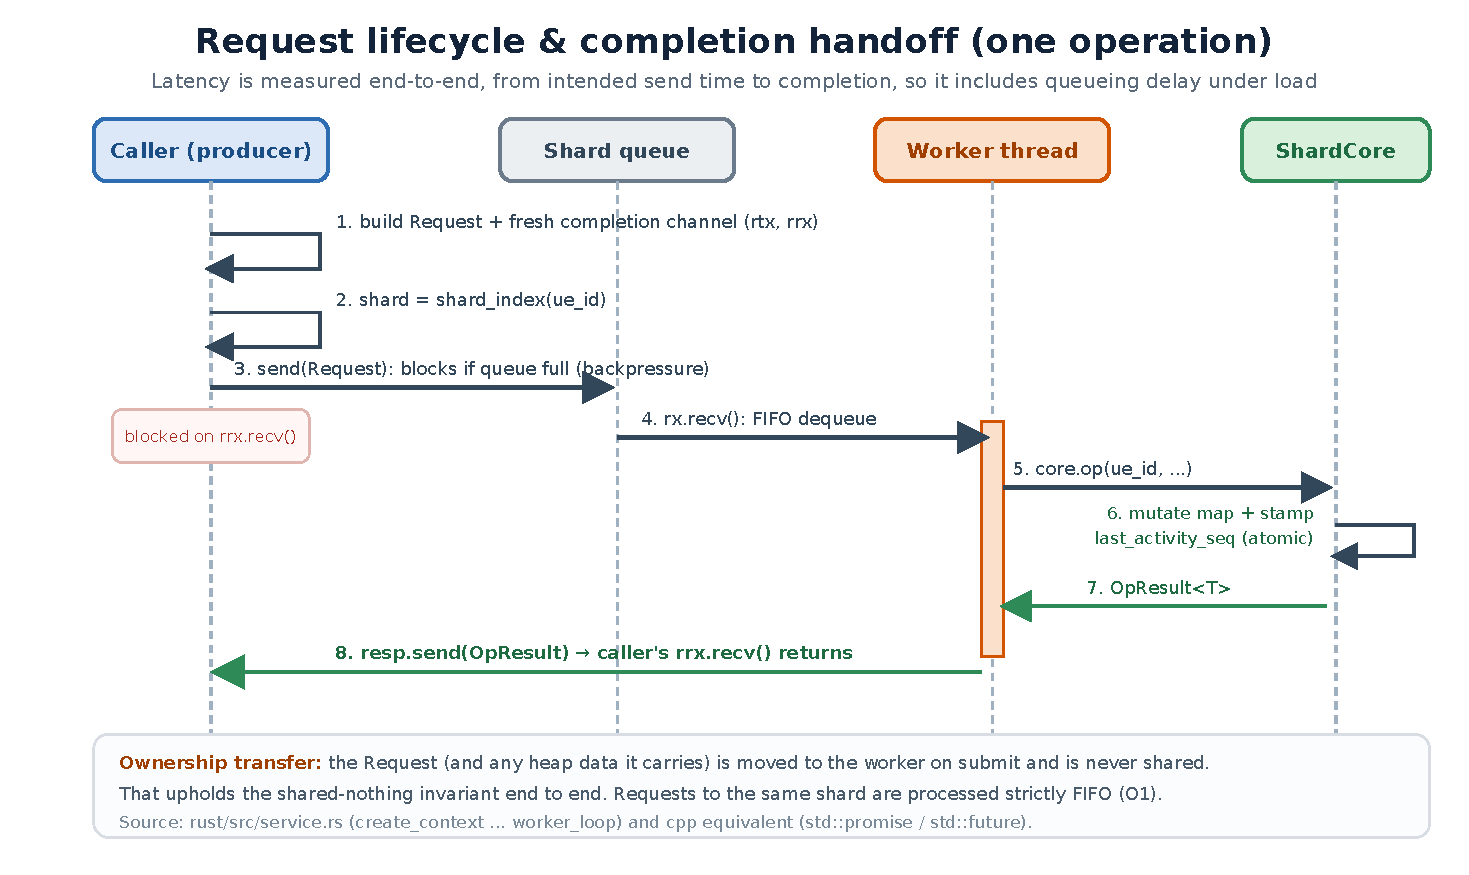
\includegraphics[width=\linewidth]{diagrams/pdf/04_request_lifecycle_sequence.pdf}
\caption[The end-to-end path of a single operation]{The end-to-end path of a single operation and the completion handoff. The caller builds
a request with a single-use completion handle, routes it by \texttt{shard\_index(ue\_id)} to the
owning shard's bounded queue (blocking if it is full), and waits. The shard's single worker
dequeues in FIFO order, executes the operation against its exclusively owned store, and writes the
result back to the completion handle. Ownership of the request is transferred to the worker on
submit and never shared. Latency is measured across the whole path.\label{fig:reqlifecycle}}
\end{figure}

\begin{figure}
\centering
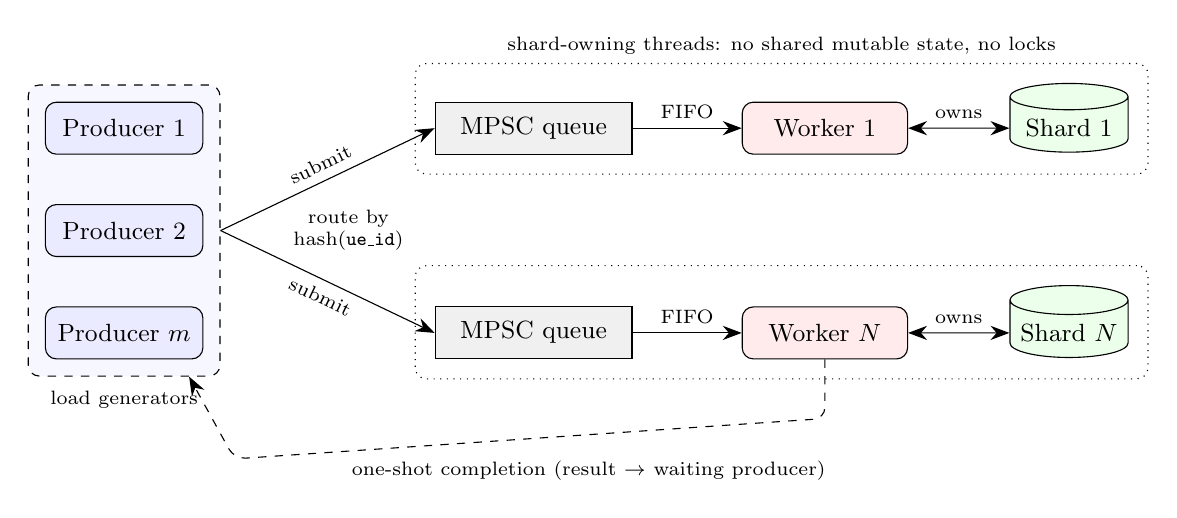
\begin{tikzpicture}[
    font=\small,
    prod/.style={draw, rounded corners, minimum width=2.0cm, minimum height=0.66cm, fill=blue!8},
    queue/.style={draw, minimum width=2.5cm, minimum height=0.66cm, fill=gray!12},
    worker/.style={draw, rounded corners, minimum width=2.1cm, minimum height=0.66cm, fill=red!8},
    store/.style={draw, cylinder, shape border rotate=90, aspect=0.25, minimum width=1.5cm, minimum height=0.85cm, fill=green!8},
    lane/.style={draw, dotted, rounded corners, inner sep=7pt},
    >={Stealth[length=2.4mm]}
  ]
  % producers, grouped in one box to avoid a tangle of crossing arrows
  \node[prod] (p1) at (0,1.3)  {Producer 1};
  \node[prod] (p2) at (0,0.0)  {Producer 2};
  \node[prod] (p3) at (0,-1.3) {Producer $m$};
  \begin{scope}[on background layer]
    \node[draw, dashed, rounded corners, fill=blue!3, fit=(p1)(p2)(p3), inner sep=6pt] (pg) {};
  \end{scope}
  \node[font=\scriptsize] at (0,-2.15) {load generators};

  % two representative shard lanes; spacing leaves room for the inline edge labels
  \node[queue] (q1) at (5.2,1.3)   {MPSC queue};
  \node[worker](w1) at (8.9,1.3)   {Worker 1};
  \node[store] (s1) at (12.0,1.3)  {Shard 1};
  \node[queue] (qn) at (5.2,-1.3)  {MPSC queue};
  \node[worker](wn) at (8.9,-1.3)  {Worker $N$};
  \node[store] (sn) at (12.0,-1.3) {Shard $N$};
  \begin{scope}[on background layer]
    \node[lane, fit=(q1)(s1)] (lane1) {};
    \node[lane, fit=(qn)(sn)] (lanen) {};
  \end{scope}
  \node[font=\scriptsize] at (8.35,2.35) {shard-owning threads: no shared mutable state, no locks};

  % submit: producer group -> each shard queue, routed by hash
  \node[font=\scriptsize, align=center, fill=white, inner sep=2pt] at (2.85,0) {route by\\ hash(\texttt{ue\_id})};
  \draw[->] (pg.east) -- (q1.west) node[midway, above, sloped, font=\scriptsize]{submit};
  \draw[->] (pg.east) -- (qn.west) node[midway, below, sloped, font=\scriptsize]{submit};

  % within-lane flow
  \draw[->]  (q1) -- node[above, font=\scriptsize]{FIFO} (w1);
  \draw[->]  (qn) -- node[above, font=\scriptsize]{FIFO} (wn);
  \draw[<->] (w1) -- node[above, font=\scriptsize]{owns} (s1);
  \draw[<->] (wn) -- node[above, font=\scriptsize]{owns} (sn);

  % one-shot completion: clean orthogonal return path below everything
  \draw[->, dashed, rounded corners=4pt]
      (wn.south) -- ++(0,-0.75) -- (1.4,-2.9) -- ($(pg.south east)+(-0.4,0)$);
  \node[font=\scriptsize] at (5.9,-3.05) {one-shot completion (result $\rightarrow$ waiting producer)};
\end{tikzpicture}
\caption[Shared-nothing, thread-per-shard architecture]{Shared-nothing, thread-per-shard architecture. Producers submit request messages to a
shard's bounded, blocking MPSC queue (selected by a pinned hash of the \texttt{ue\_id}) and wait
on a single-use completion handle. Each shard is read and written by exactly one worker thread,
so there are no locks on context state. Blocking on a full queue is what makes overload
observable as tail latency.\label{fig:arch}}
\end{figure}

\section{Architectural choices and technology stack}
The C++ side uses CMake with Ninja, the standard library, and \texttt{std::thread}. The Rust
side uses Cargo and the stable toolchain. To keep the comparison a language comparison
rather than an allocator comparison, both link the same memory allocator: C++ links the
system \texttt{jemalloc} and Rust installs a \texttt{jemalloc} global allocator (from
\texttt{tikv-jemallocator}), with a system-allocator build retained on each side as a
control. Both record latency through the same high-dynamic-range (HDR) histogram
algorithm~\cite{tene_hdrhistogram}, configured identically (range $[1\,\text{ns},
3.6\,\text{s}]$, three significant figures). Rust uses the canonical \texttt{hdrhistogram}
crate and C++ uses a header-only port of the same bucketing algorithm, validated against a
known distribution. Build optimisation is matched as closely as the two toolchains allow:
the Rust release profile is pinned to \texttt{opt-level~=~2} to match the C++ \texttt{-O2}
build.

\section{Implementation details}\label{sec:impldetails}
\label{sec:impl}
Both implementations follow the frozen specification field-for-field, and both are small
enough to be read end to end. The C++ core is $\CppRawLines$ lines across eight headers and two
translation units, the Rust core $\RustRawLines$ lines across eight modules. Discarding blank
lines and comments leaves $\CppNloc$ and $\RustNloc$ respectively. Both counts describe the
configuration the campaign measures: the two attribution probes of Section~\ref{sec:idioms} are
switched on by a build flag, and the conditional blocks that select them are excluded, since
counting them would describe neither the compared build nor the probe.

The Rust version is therefore the larger of the two, by $\RawRise\%$ in raw lines and
$\NlocRise\%$ in code lines. That is worth stating plainly rather than leaving it to a footnote, for two reasons. Line
count is one of the software-quality proxies this study set out to collect, and the difference
is not incidental verbosity: it is the net of several forced idioms pulling in opposite
directions, which Section~\ref{sec:idioms} decomposes file by file. The remainder of this
section works outward from the data model to the concurrency machinery, and reports the measured
consequences of each language-forced divergence as it arises.

\subsection{The UE context and the state machine}\label{sec:uecontext}
Each UE context stores its identifier, lifecycle state (a four-value enumeration
\texttt{Idle}, \texttt{Connected}, \texttt{Reconfiguring}, \texttt{Released}), serving cell,
RRC transaction id, a fixed 32-byte dummy security context, a dynamic list of up to eight data
radio bearers, and two counters (messages handled and an activity sequence number). The data
radio bearer list is deliberately a growable container (\texttt{std::vector} / \texttt{Vec})
and not a fixed array, so that the allocator study (RQ3) observes realistic per-context
allocation. Reads return an immutable snapshot (a \texttt{UeContextView}) copied out of the
worker rather than a reference into live shard state, which preserves the shared-nothing
guarantee and keeps the two implementations semantically identical.
Figure~\ref{fig:datamodel} gives the record and the read path in full.

Identical field declarations do not, however, produce identical objects. Measured on the
evaluation host, a \texttt{UeContext} occupies $\CppUeCtxBytes$~bytes in C++ but only
$\RustUeCtxBytes$~bytes in Rust.
The difference is entirely layout policy. C++ guarantees that non-static data members are laid
out in declaration order, so the one-byte \texttt{state} enumeration sitting between the
eight-byte identifier and the four-byte cell id forces $\CppUeCtxStatePad$~bytes of padding, and the
32-byte security key ending at offset $\CppUeCtxKeyEnd$ forces a further $\CppUeCtxKeyPad$ before the eight-byte-aligned
bearer vector. Rust, absent a \texttt{\#[repr(C)]} annotation, is free to reorder fields and
does so, packing the small scalars together and eliminating both holes. The specification
deliberately does not try to erase this difference: pinning the Rust layout with
\texttt{\#[repr(C)]} would penalise Rust for nothing but conformity to a C++ padding rule,
while hand-reordering the C++ declarations would be an optimisation the specification asks of
neither side. It is instead recorded as a language-level effect and bounded, at the $\SweepUes$
active UEs used in the sweep the $\UeCtxGapBytes$-byte gap accounts for roughly $\UeCtxGapTotalKB$~kB, against resident
set sizes measured in megabytes, so it is immaterial to the RQ3 comparison.

\begin{figure}
\centering
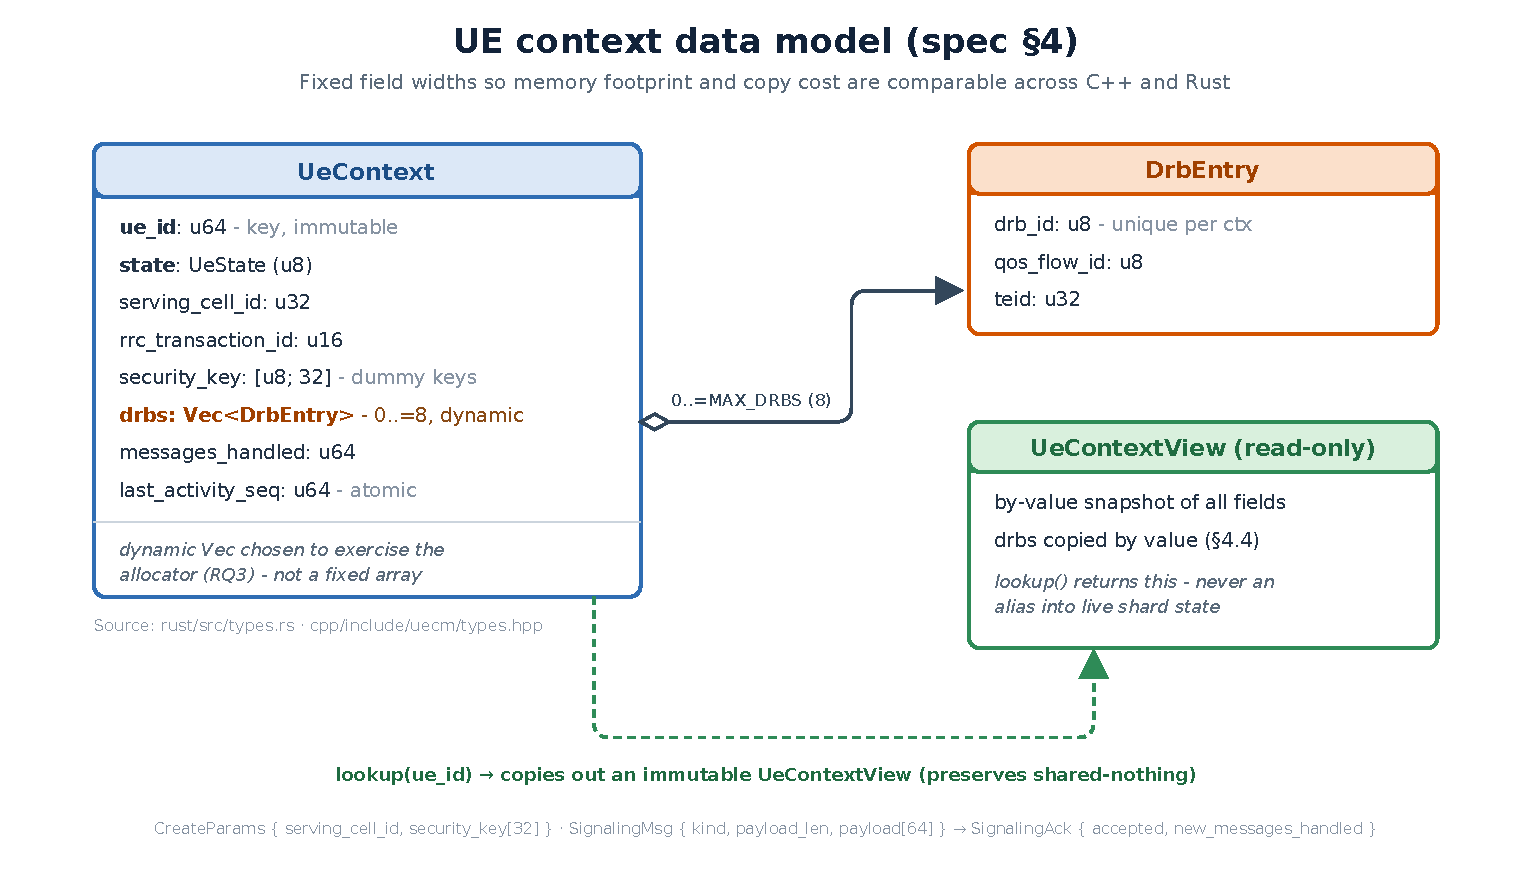
\includegraphics[width=0.92\linewidth]{diagrams/pdf/05_data_model.pdf}
\caption[The shared UE-context data model]{The UE-context data model shared by both implementations. Field widths are fixed so that
memory footprint and copy cost are comparable across languages. The data-radio-bearer list is a
dynamic \texttt{Vec}/\texttt{std::vector} on purpose, to exercise the allocator for RQ3.
\texttt{lookup} returns an immutable \texttt{UeContextView} copied out by value rather than an
alias into live shard state, preserving the shared-nothing guarantee.\label{fig:datamodel}}
\end{figure}

That record is driven by the lifecycle of Figure~\ref{fig:fsm}, realised as a single guarded
transition per operation, with Table~\ref{tab:transitions} giving the implemented table in full.
Two properties hold uniformly and are what make the two implementations comparable op for op.
First, every operation validates before it mutates: the guard sequence checks the identifier,
then locates the context, then tests the state, and returns the corresponding \texttt{OpError}
before touching any field, so a rejected operation leaves the context bit-identical to what it
was. Second, no operation can partially succeed, because each performs at most one mutation
after the last guard has passed.

Two behaviours deserve explicit mention because the table alone hides them. The
\texttt{Released} state is never actually stored: \texttt{release\_context} erases the entry
from the shard map outright, so \texttt{Released} is a transient terminal label in the
specification rather than a resting value an implementation can be found in, and a second
release therefore returns \texttt{NotFound} instead of \texttt{InvalidState}.
And \texttt{abort\_reconfigure} restores the \emph{state} to \texttt{Connected} but does not
restore the serving cell that \texttt{begin\_reconfigure} overwrote with the handover target.
This is a deliberate simplification, the model carries no saved pre-handover cell to roll back
to, but it is a semantic commitment and not an oversight, and both implementations make it
identically, which is what the parity suite of Section~\ref{sec:parity} checks.

\begin{table}
\centering
\small
\caption[The implemented state-transition table]{The implemented state-transition table, identical in both languages. Every operation
additionally returns \texttt{InvalidArgument} for a zero \texttt{ue\_id}, and a rejected
operation leaves the context unmodified. \texttt{Released} is never stored: release erases
the entry.\label{tab:transitions}}
\begin{tabular}{@{}l l l R{0.31\linewidth}@{}}
\hline\hline
Operation & Required state & Resulting state & Errors \\
\hline
\texttt{create\_context}       & context absent   & \texttt{Idle}          & \texttt{AlreadyExists}, \texttt{CapacityExceeded} \\
\texttt{setup\_connection}     & \texttt{Idle}          & \texttt{Connected}     & \texttt{NotFound}, \texttt{InvalidState} \\
\texttt{handle\_signalling}     & \texttt{Connected}     & \texttt{Connected}     & \texttt{NotFound}, \texttt{InvalidState} \\
\texttt{add\_drb}              & \texttt{Connected}     & \texttt{Connected}     & \texttt{NotFound}, \texttt{InvalidState}, \texttt{CapacityExceeded}, \texttt{AlreadyExists} \\
\texttt{begin\_reconfigure}    & \texttt{Connected}     & \texttt{Reconfiguring} & \texttt{NotFound}, \texttt{InvalidState} \\
\texttt{complete\_reconfigure} & \texttt{Reconfiguring} & \texttt{Connected}     & \texttt{NotFound}, \texttt{InvalidState} \\
\texttt{abort\_reconfigure}    & \texttt{Reconfiguring} & \texttt{Connected}     & \texttt{NotFound}, \texttt{InvalidState} \\
\texttt{release\_context}      & any live state   & entry erased           & \texttt{NotFound} \\
\texttt{lookup}                & any live state   & unchanged              & \texttt{NotFound} \\
\hline
\end{tabular}
\end{table}

\subsection{Sharding, the store, and the bounded queue}
To prevent the standard library hashers from becoming an accidental language advantage, both
sides pin their hashing. Shard assignment applies the SplitMix64 finalizer to the
\texttt{ue\_id}, three xor-shift and multiply rounds with the constants
\texttt{0xBF58476D1CE4E5B9} and \texttt{0x94D049BB133111EB}, before reducing modulo the shard
count. The finalizer matters because the workload draws sequential identifiers, which a naive
modulo would map onto shards in a fixed repeating pattern. Diffusing the identifier first makes
the offered load per shard uniform in both languages by construction rather than by luck.

The per-shard container is each language's standard hash map (\texttt{std::unordered\_map} /
\texttt{std::collections::HashMap}), but the default hashers are bypassed. They differ too much
to leave in place: C++'s \texttt{std::hash<uint64\_t>} is typically the identity function, while
Rust's default \texttt{SipHash-1-3} is cryptographically strong and correspondingly slower.
Keeping them would have measured a standard-library choice rather than a language. Both are
therefore keyed through a pinned FNV-1a 64-bit hash over the eight little-endian bytes of the
identifier, and a test checks that the Rust \texttt{BuildHasher} produces a digest bit-identical
to the reference \texttt{fnv1a\_64}.

Both maps reserve an initial capacity of $4\,096$ entries at start-up so that steady-state
measurements are not disturbed by rehashing. The remaining configuration is likewise shared:
the default eight shards, a queue bound of
$1\,024$ requests per shard, at most eight bearers and a 64-byte signalling payload per
context, and a ceiling of $200\,000$ contexts per shard. Only the shard count is varied from
these defaults, and only by the campaign, which sets it to match the cores it is given.

The bounded blocking queue is where the two standard libraries diverge most sharply. Rust
provides the primitive the specification calls for directly: \texttt{sync\_channel(capacity)} is
a bounded multi-producer, single-consumer channel whose \texttt{send} blocks when the queue is
full and whose \texttt{recv} blocks when it is empty, which is precisely the required
backpressure semantics in a single call. The C++ standard library, through C++23, offers no
bounded blocking queue at all, so the same semantics are assembled by hand from a
\texttt{mutex}, two \texttt{condition\_variable}s and a \texttt{std::queue}, in a class of $45$
lines.

The point of the comparison is not that the C++ code is badly written. It is short, it uses
the predicate form of \texttt{wait} so spurious wakeups are handled correctly, and it releases
the lock before notifying. The point is that it exists at all. Every one of those lines is a
place where a concurrency defect could be introduced, and the correctness argument for it,
that the two condition variables are never confused, that the predicates match the
notifications, that no wakeup is lost, is carried by the author rather than by the compiler or
the library. This is the same asymmetry the fault-injection study of Chapter~\ref{chapter:eval}
measures, appearing here in ordinary, non-defective code instead of in a deliberately injected
bug.

\subsection{Requests, responses, and the service lifecycle}\label{sec:tagged}
\label{sec:request}
The message type carried through that queue is the second forced divergence. Rust models a
request as an \texttt{enum} with one variant per
operation. Each variant carries exactly its own arguments plus a \texttt{Sender} parameterised
by exactly that operation's result type. C++ has no equivalent of a payload-carrying
enumeration in the standard idiom used here, so a request is a tagged struct: an
\texttt{OpKind} discriminant alongside \emph{every} argument field any operation might need,
paired with a single \texttt{std::promise} whose value type must therefore be a
\texttt{std::variant} over all four possible result types.

This has three measurable consequences. The first is size: a \texttt{Request} is $\CppRequestBytes$~bytes
in C++ against $\RustRequestBytes$ in Rust, because the C++ struct always carries the create parameters, the
$\SignalingMsgBytes$-byte signalling message, the bearer entry, and the reconfiguration parameters, whether or
not the operation in flight uses them, while the Rust enum is sized by its largest variant
alone. With the default eight shards holding up to $1\,024$ requests each, that is roughly $\CppQueueResidentMB$~MB of
queue-resident request storage at full occupancy against $\RustQueueResidentMB$~MB. The second is a copy cost
paid on every submission, since the unused fields are default-initialised and moved along with
the used ones. The third, and the most interesting for the thesis's argument, is a type-safety
gap: the C++ caller must recover its typed result from the variant with
\texttt{std::get<OpResult<T>>}, which throws \texttt{std::bad\_variant\_access} if the worker
ever writes an alternative the caller did not expect. That exception cannot fire in the
present code, because each \texttt{OpKind} is handled by exactly one branch that stores the
matching alternative, but the invariant guaranteeing it is maintained by inspection across two
files. In Rust the same invariant is discharged by construction: because the sender embedded
in each variant is already typed, there is no response union, nothing to unwrap, and no
runtime dispatch on the way back.

Starting the service allocates the shards, spawns one worker thread per shard, and hands each
worker exclusive ownership of its store. The request path is then as described in
Section~\ref{sec:concurrency}. Shutdown is the more delicate half, because it must terminate
workers that are blocked on an empty queue without abandoning requests that are still in
flight. Both implementations solve it the same way, with an in-band \texttt{Stop} sentinel:
one \texttt{Stop} request is pushed onto each shard's queue, and because the queue is strictly
FIFO, every request already enqueued ahead of it is executed and completed before the worker
observes the sentinel and returns. No separate closed flag, timeout, or drain API is required,
and no completion handle is left unfulfilled. The worker threads are then joined, so shutdown
returns only once every shard has actually stopped.

Both languages tie this to object destruction, and the mechanism is one of the few places
where the two are near-identical: the C++ destructor calls \texttt{shutdown()}, and Rust's
\texttt{Drop} implementation does the same, so a service that goes out of scope cannot leave
detached threads behind. Both guard against double invocation with a \texttt{running} flag,
making shutdown idempotent.

The window those two calls delimit is a precondition on every operation, and it is stated as one:
an operation submitted before \texttt{start()} or after \texttt{shutdown()} is a caller error, not
a runtime condition, so it is reported out of band rather than widening the closed
\texttt{OpError} set of Section~\ref{sec:parity}: C++ throws \texttt{std::logic\_error}, Rust
panics. Making it explicit was not a formality. The specification originally prohibited the call
without either implementation checking, and the two languages did not fail alike in the gap. The
episode is reported with the safety results in Section~\ref{sec:safetyresults}, because a defect
found in code written to be correct carries evidence an injected one cannot. The remaining ownership discipline is what upholds the
shared-nothing invariant end to end: a request is moved into the queue rather than copied,
carrying its completion handle with it, so at no point do the producer and the worker both
hold a usable reference to the same request. In C++ this is enforced by making
\texttt{Request} move-only, a property it acquires automatically from the move-only
\texttt{std::promise} it contains. In Rust it follows from ordinary move semantics, and the
compiler rejects any attempt to use the request after submission. The only shared mutable
state in either implementation is the atomic activity counter, held by reference in C++ and
as a cloned \texttt{Arc<AtomicU64>} in Rust, and incremented with relaxed ordering because
nothing branches on its value.

\subsection{Forced idioms, and what the two cores cost}
\label{sec:idioms}
Where the two languages must diverge to satisfy the same requirement, the deviation is
recorded in the specification's forced-idiom log so that it can be weighed rather than
silently absorbed into the results. Table~\ref{tab:idioms} collects the log in full, and the
preceding subsections have already quantified the two entries with measurable consequences.

\begin{table}
\centering
\small
\caption[The forced-idiom log]{The forced-idiom log: every point at which the two implementations diverge in order
to satisfy the same specification requirement, with the measured consequence where there is
one.\label{tab:idioms}}
\begin{tabular}{@{}R{0.20\linewidth} R{0.36\linewidth} R{0.36\linewidth}@{}}
\hline\hline
Concern & C++ & Rust \\
\hline
Result type & \texttt{std::expected<T, OpError>} & \texttt{Result<T, OpError>} \\
Request & tagged struct: discriminant plus every argument field ($\CppRequestBytes$\,B) & \texttt{enum}, one variant per operation, carrying only its own arguments ($\RustRequestBytes$\,B) \\
Response & \texttt{std::variant} of four result types, unwrapped by the caller with \texttt{std::get} & none needed: each variant carries a sender of its own result type \\
Bounded queue & hand-written \texttt{mutex} plus two \texttt{condition\_variable}s ($45$ lines) & \texttt{sync\_channel(capacity)} \\
Completion & \texttt{std::promise} / \texttt{std::future} & a fresh \texttt{mpsc::channel()} per request \\
Per-shard map & \texttt{std::unordered\_map} with an \texttt{FnvHash} functor & \texttt{HashMap} with an \texttt{FnvBuildHasher} \\
Activity counter & \texttt{std::atomic<uint64\_t>} held by reference & \texttt{Arc<AtomicU64>} cloned into each worker \\
Teardown & destructor calls \texttt{shutdown()} & \texttt{Drop} calls \texttt{shutdown()} \\
Optimisation level & \texttt{-O2} & \texttt{opt-level = 2} \\
\hline
\end{tabular}
\end{table}

The log also explains the line-count difference reported at the head of this section, and it
is more informative than the net figure suggests, because the contributions do not all point
the same way. Table~\ref{tab:loc} decomposes the $\LocGap$-line gap by concern. Rust is
substantially \emph{shorter} in exactly one place, the bounded queue, where it needs no code
at all against 45 lines of C++, and longer almost everywhere else, with three contributions
accounting for most of the excess.

The largest is the service module, for the reason developed above: because the C++ response is a
single \texttt{variant}, all ten public operations funnel through one shared \texttt{submit}
helper and each typed wrapper shrinks to two or three lines, while Rust's per-variant typed
sender admits no such helper without generics, so each operation repeats the sequence of
creating a completion channel, constructing its variant, sending, and receiving. The next, and
the one that best illustrates the trade-off, is hashing: C++ satisfies
\texttt{std::unordered\_map}'s hasher requirement with a five-line functor wrapping
\texttt{fnv1a\_64}, whereas Rust must supply the whole trait apparatus, every line of it
boilerplate, buying a statically dispatched, type-checked hasher rather than a conventionally
shaped callable. The third is the module tree and public re-export list, work C++ gets
implicitly from its header structure.

None of this is a defect on either side, and none of it is visible in the performance figures.
It is the kind of engineering cost the forced-idiom log exists to surface: Rust spends source
lines on trait machinery and call-site repetition to obtain guarantees the compiler can check,
and recovers a large part of that spend wherever its standard library happens to provide a
primitive that C++'s does not.

Counting lines, however, answers only half the question a reviewer of either codebase would
ask, because it treats a line of boilerplate and a line of branching as the same thing.
Table~\ref{tab:complexity} therefore adds cyclomatic complexity, measured by
\texttt{lizard}~\cite{lizard} over both cores. Applying one tool to both languages is what makes
the figures comparable: it applies the same definition of a decision point on both sides,
whereas each language's native tooling would count somewhat different things. The two measures
point in opposite directions. Rust is $\NlocRise\%$ longer than C++ by code lines, but its
total cyclomatic complexity is $\CcnTotalDrop\%$ \emph{lower}, $\RustCcnTotal$ against
$\CppCcnTotal$, spread over slightly more functions ($\RustFuncs$ against $\CppFuncs$). Both
cores are undemanding by the usual thresholds and both have a median per-function complexity
of one, so the aggregate is carried by a small number of functions at the top.

That is where the difference sits, and it traces to a divergence already described rather than
to anything diffuse. The most complex function in the C++ core is
$\CppCcnMaxFn$ at $\CppCcnMax$, more than twice its Rust counterpart's $\RustCcnMax$. It
switches on the \texttt{OpKind} discriminant and then stores the matching alternative into the
response \texttt{variant}, so the tagged-struct design of Section~\ref{sec:tagged} concentrates
the whole dispatch, and the correctness argument that goes with it, into one branch-heavy
function. Rust's per-variant typed sender removes the return-path dispatch entirely, which is
why its worker has nothing comparable to unwrap. The trade is therefore sharper than the line
count alone suggested. The extra lines Rust spends buy back branching in the one place where
branching is hardest to review, and the \texttt{std::bad\_variant\_access} invariant that
Section~\ref{sec:tagged} noted is maintained by inspection across two files lives inside
precisely the function this measurement flags.

\begin{table}
\centering
\small
\caption[Size and cyclomatic-complexity proxies for the two cores]{Size and cyclomatic-complexity proxies for the two cores, measured with
\texttt{lizard}~\cite{lizard} applied identically to both languages. Benchmark drivers, tests,
conformance runners, the FFI seam, and the probe-conditional blocks of
Section~\ref{sec:idioms} are excluded. Only the compared code the parity contract constrains is
counted. Complexity is one plus the number of decision points in a function. The line count is
NLOC as \texttt{lizard} defines it, which also discounts brace-only and preprocessor lines. It
is the same measurement quoted at the head of
Section~\ref{sec:impldetails}.\label{tab:complexity}}
\begin{tabular}{@{}l r r@{}}
\hline\hline
Measure & C++ & Rust \\
\hline
Files & 10 & 8 \\
Functions & 37 & 42 \\
Lines of code (blank and comment lines excluded) & 517 & 621 \\
Total branching complexity & 95 & 83 \\
Mean complexity per function & 2.6 & 2.0 \\
Median complexity per function & 1 & 1 \\
Most complex function & 13 (\texttt{worker\_loop}) & 6 (\texttt{add\_drb})
\\
\hline
\end{tabular}
\end{table}

\begin{table}
\centering
\small
\caption[Where the line-count difference between the cores comes from]{Where the $\LocGap$-line difference between the two cores comes from, by concern (raw
lines, including comments. C++ figures merge header and translation unit. Probe-conditional
blocks excluded as in Section~\ref{sec:impldetails}). Rust is shorter
only where its standard library supplies a primitive C++ lacks.\label{tab:loc}}
\begin{tabular}{@{}R{0.38\linewidth} r r r@{}}
\hline\hline
Concern & C++ & Rust & $\Delta$ \\
\hline
Service (queues, workers, API)    & $234$ & $278$ & $+44$ \\
Hashing (functor vs.\ trait pair) & $36$  & $70$  & $+34$ \\
Module tree and re-exports        & $0$   & $26$  & $+26$ \\
Data model                        & $73$  & $85$  & $+12$ \\
Message types                     & $48$  & $60$  & $+12$ \\
Configuration                     & $18$  & $29$  & $+11$ \\
Shard core (state machine)        & $182$ & $188$ & $+6$ \\
Error model                       & $32$  & $26$  & $-6$ \\
Bounded queue                     & $45$  & $0$   & $-45$ \\
\hline
Total                             & $\CppRawLines$ & $\RustRawLines$ & $+\LocGap$ \\
\hline
\end{tabular}
\end{table}

One property of the Rust core is not a cost at all, and it closes this section because it is what
the costs above were paid for. The Rust library contains \emph{no} \texttt{unsafe} code at all, a property verified
mechanically over the crate. Safe Rust therefore guarantees data-race freedom for this core at
compile time through the \texttt{Send} and \texttt{Sync} traits: the shard store is owned by a
single worker and never shared, the request type is moved across the thread boundary, and the
one piece of genuinely shared state, the activity counter, is an atomic. No runtime sanitiser
is needed to establish any of this, and no test coverage is required for it to hold. The C++
implementation performs no manual memory management beyond STL containers and no explicit
locking outside the queue class, and it was verified data-race free under ThreadSanitizer.

The two statements are not, however, evidence of the same kind, and the difference is the
thesis's central safety claim in miniature. The Rust property is a theorem about the program,
discharged by the compiler on every ordinary build and covering every execution. The C++
property is an observation about the executions a particular instrumented binary happened to
take, and it would have to be re-established after any change, on a build most projects do not
run by default. Quantifying exactly how far apart those two kinds of assurance are is the
purpose of the fault-injection study in Chapter~\ref{chapter:eval}.

\section{Public API and operation semantics}
Both implementations expose the same small, lifecycle-oriented API against the shared
specification, so that the surface a caller sees is identical up to each language's naming
conventions. A service is created with a fixed shard count and a per-shard queue bound.
Thereafter callers invoke context operations, create, setup, handle-signalling, add-bearer,
reconfigure begin/complete/abort, release, and state lookup, each identified by the target
\texttt{ue\_id}. Every operation is \emph{total} and \emph{typed}: it returns a success value or
a typed \texttt{OpError} drawn from a closed five-value enumeration (\texttt{NotFound},
\texttt{AlreadyExists}, \texttt{InvalidState}, \texttt{CapacityExceeded} and
\texttt{InvalidArgument}), and an operation that is illegal for the context's
current state (Figure~\ref{fig:fsm}) returns the corresponding error and leaves the context
unchanged rather than mutating it or signalling failure out of band. This choice matters for
fairness as much as for correctness: because neither implementation uses exceptions or error
codes as a hidden control-flow channel, the cost and the control flow of the failure path are
visible and identical on both sides, and the same conformance vectors (Section~\ref{sec:parity})
can assert op-for-op agreement on both the returned value and the resulting state.

\section{Parity verification}
\label{sec:parity}
Because the whole comparison rests on the two versions being functionally identical, parity
is tested rather than assumed. A language-neutral conformance suite expresses test vectors as
sequences of operations with their expected results and an expected post-state summary. A
runner in each language executes the vectors and emits a canonical transcript, and the two
transcripts are diffed for op-for-op agreement. The seeded suite covers the full error model,
the reconfiguration begin/complete/abort paths, data-radio-bearer fill and overflow, and
shard-assignment determinism. Both implementations currently pass and agree. The benchmark
workloads add a second, independent parity signal: the mixed workload's per-operation-kind
counts are verified to be identical across languages for a given seed and active-UE
population, confirming that both implementations are driven along exactly the same code paths.

Two things bound what that establishes, and both are addressed rather than conceded. A
cross-diff of two implementations cannot distinguish ``both correct'' from ``both wrong in the
same way'', which is the failure mode a shared specification and a single author make most
likely; and the expected results in the hand-written vectors were derived from the
specification by the same person who wrote the implementations. A third implementation of the
same written specification therefore acts as an independent oracle. It is written in Python,
shares no code with either language, and first has to reproduce all $\ConfHandOps$ hand-derived
expectations before it is allowed to generate any of its own. It then generates randomised
operation sequences under several profiles (realistic lifecycles, adversarial sequences
weighted towards illegal transitions, sequences that sit on the capacity limits, and sequences
that stress shard assignment), with every expected result computed by the model. A campaign
of roughly $\ConfGenOps$ generated operations produced no divergence: the two implementations
agree with each other and with an independent reading of the specification, on sequences nobody
chose. Because the generator is seeded and deterministic, any future divergence is a
permanently reproducible regression rather than an anecdote.

Three further checks bound the suite from other directions. The specification's transition
matrix is enumerated exhaustively rather than sampled: every operation applied to a context in
every state it can occupy, asserting the exact error, the resulting state on success, and the
absence of any field change on failure, including the error precedences the specification
leaves unordered. The C++ implementation is then run under AddressSanitizer, ThreadSanitizer
and UndefinedBehaviorSanitizer across that whole suite, and reports nothing, which matters for
fairness: safe Rust carries data-race and memory-safety freedom by construction, so without
this the C++ arm's equivalent property would rest on not having failed yet rather than on
having been checked. Miri, run over the Rust state-machine suite, likewise reports no
undefined behaviour. Finally, the suite's reach is measured rather than asserted, because a
negative result from a sanitiser is only as broad as the code that ran: line coverage of the
C++ library is $\CppLineCov\%$ and of the Rust library $\RustLineCov\%$, with both implementations' core
operation processors and service facades fully covered. The two figures are not strictly
comparable, because \texttt{gcov} and \texttt{llvm-cov} do not resolve an executable line alike.
On the finer-grained regions \texttt{llvm-cov} counts, the Rust figure is $\RustRegionCov\%$.
Each bounds the claims made about its own implementation.

\chapter{Experimental Setup and Evaluation\label{chapter:eval}}

\section{Testbed configuration\label{sec:testbed}}
Two execution environments must be distinguished, because the thesis deliberately reports
results of two different evidential strengths and the distinction rests entirely on where
they were produced.

\paragraph{The environment used.}
All performance results reported in this chapter were measured on the dedicated dual-socket server
itemised in Table~\ref{tab:testbed}, with the benchmark pinned so that every worker and every
producer owns a core and none contends with the operating system. Every run captures its own
environment record (CPU model and topology, kernel, compiler and toolchain versions, and the
frequency, turbo, and multithreading settings) alongside the measurement data, so the conditions
of a measurement travel with it.

One property of this host has to be stated plainly because it bounds the tail claims below: it is
a virtual machine. The environment record identifies a KVM guest, and two consequences follow.
The CPU frequency governor and turbo state are host-controlled and not merely unset but
unobservable from inside the guest, so frequency stability is assumed rather than enforced. And
the record shows non-zero CPU steal, on the order of ten milliseconds of vCPU time per second:
small in aggregate, but the same order as the tail latencies being measured, and not removable
from inside the guest. The cores were also not removed from the scheduler with
\texttt{isolcpus}, so a benchmark thread can still lose its core to other work.

This is a substantially better instrument than a shared development laptop, which is what an
earlier pass of this campaign used: the cores are homogeneous and server-class, nothing else of
consequence runs on the machine, and the run-to-run dispersion at p99 fell by more than an order
of magnitude between the two. It is not the bare-metal host the protocol below specifies.

\paragraph{The protocol the performance campaign still lacks.}
Testbed-grade tail figures require a dedicated bare-metal host, and the protocol for one is
specified, scripted, and published so that it can be executed without further design work
(\texttt{bench/TESTBED.md}), its requirements given in the right-hand column of
Table~\ref{tab:testbed}. What executing it would add is narrower than it once was. Three of the
four things it was going to buy have been obtained without it: the saturation knee, the shape of
the overload cliff
(Section~\ref{sec:overload}), and the replication of the resource comparisons across the allocator
control (Section~\ref{sec:resources}). What remains is the far tail \emph{below} saturation,
where the confidence interval on a single variant's p99 is still several times the spread between
all four variants, and where steal and scheduler preemption are the plausible cause, not
anything either language does. That one result is therefore reported as unresolved rather than as
a null, and the mechanism to resolve it belongs to the machine and not to the analysis.

\paragraph{Measurement discipline common to both.}
Independently of the host, each sweep point is repeated \NRepeats{} times and reported as a
median with a bootstrap $95\%$ confidence interval rather than as a single run, and the four
language$\times$allocator variants are interleaved within each repeat so that thermal or
background drift affects them equally instead of biasing one. That interleaving is what makes
a contended host tolerable for a \emph{comparative} conclusion even though it invalidates the
absolute numbers: interference is shared, not assigned. Throughput is counted over the measured
phase alone, with the warm-up iterations excluded from both the numerator and the denominator,
so that achieved throughput is directly comparable with offered load.

The division Table~\ref{tab:testbed} draws is not between important and unimportant results but
between those that are properties of the compilers and the source, which this host establishes as
firmly as any would, and those that are properties of the machine, which it cannot.

\begin{table}
\centering
\small
\caption[The host used and the testbed protocol still to be executed]{The host the reported
results were measured on, against the protocol that testbed-grade tail figures require
(\texttt{bench/TESTBED.md}). The rows where the two columns agree are properties of the source and
the compilers. The rows where they differ are what a bare-metal campaign would still buy. Only the
last of those differences now costs a result, because the saturation knee and the resource
comparisons were resolved on this host: what remains is the far tail below
saturation.\label{tab:testbed}}
\renewcommand{\arraystretch}{1.2}
\begin{tabular}{@{}R{0.22\linewidth} R{0.35\linewidth} R{0.35\linewidth}@{}}
\hline\hline
Aspect & Used for the results reported here & Required for testbed-grade tail figures \\
\hline
Host & Dedicated dual-socket server, $2\times$ Xeon E5-2680~v4, $16$ cores, one NUMA node & Same class of machine, without the hypervisor \\
Virtualisation & KVM guest: frequency and turbo host-controlled and unobservable & None. Governor and turbo set and verified \\
CPU steal & Non-zero, order $10$~ms of vCPU time per second & None \\
Kernel & Rocky Linux~8.10, distribution kernel & Same, with \texttt{isolcpus} and \texttt{nohz\_full} on the benchmark cores \\
Toolchain & \texttt{g++~15.1.1}, \texttt{rustc~1.97} & \texttt{g++~15.1.1}, \texttt{rustc~1.97} \\
CPU pinning & Cores $2$--$15$ via \texttt{taskset}, $7$ shards, $7$ producers & Same, on cores also removed from the scheduler \\
Simultaneous multithreading & Absent on this processor & Absent or disabled \\
Warm-up & Initial fraction of each run discarded & Initial fraction of each run discarded \\
Repeats and interleaving & \NRepeats{} repeats, four variants interleaved per repeat & \NRepeats{} repeats, four variants interleaved per repeat \\
Environment capture & \texttt{bench/capture\_env.sh}, stored with each result & \texttt{bench/capture\_env.sh}, stored with each result \\
Hardware counters & Unavailable in the guest & Available: the clearest instrumentation gap \\
\hline
Adequate for & Parity, fault injection, FFI structure, the saturation knee and the overload comparison, and the resource comparisons & Additionally the far tail below saturation, and the mechanism behind the resource and operation results \\
\hline
\end{tabular}
\end{table}

\section{Workload and evaluation measurements\label{sec:workload}}
A synthetic but spec-justified telecom workload is generated by a deterministic driver shared
in structure by both implementations, so that the two versions are exercised along identical
code paths. Two workloads are provided. The \emph{signal} workload preloads a population of
connected UEs and then hammers the \texttt{handle\_signalling} hot path, isolating steady-state
per-message latency. The \emph{mixed} workload is a pinned RAN lifecycle generator that walks
each UE through a realistic procedure sequence, context creation, connection setup, signalling,
bearer setup, reconfiguration/handover (begin/complete/abort), and release, using a fixed
SplitMix64 draw order and a per-slot expected-state model so that every emitted operation is
valid. Because the draw order is fixed, the per-operation-kind counts are identical in C++ and
Rust for a given active-UE population and seed, which doubles as the parity signal described in
Section~\ref{sec:parity}. The control parameters are the target event rate and the number of
active UEs, swept from nominal load through saturation and overload. A fixed send schedule with
histogram correction is used so that coordinated-omission bias is avoided when the system
stalls~\cite{schroeder2006openclosed,tene_hdrhistogram}. Three measurement campaigns are run: a load sweep for
performance, the fault-injection study, and an FFI migration prototype.
Figure~\ref{fig:workload} shows the two workloads and the procedure sequence the mixed one
walks.

\begin{figure}
\centering
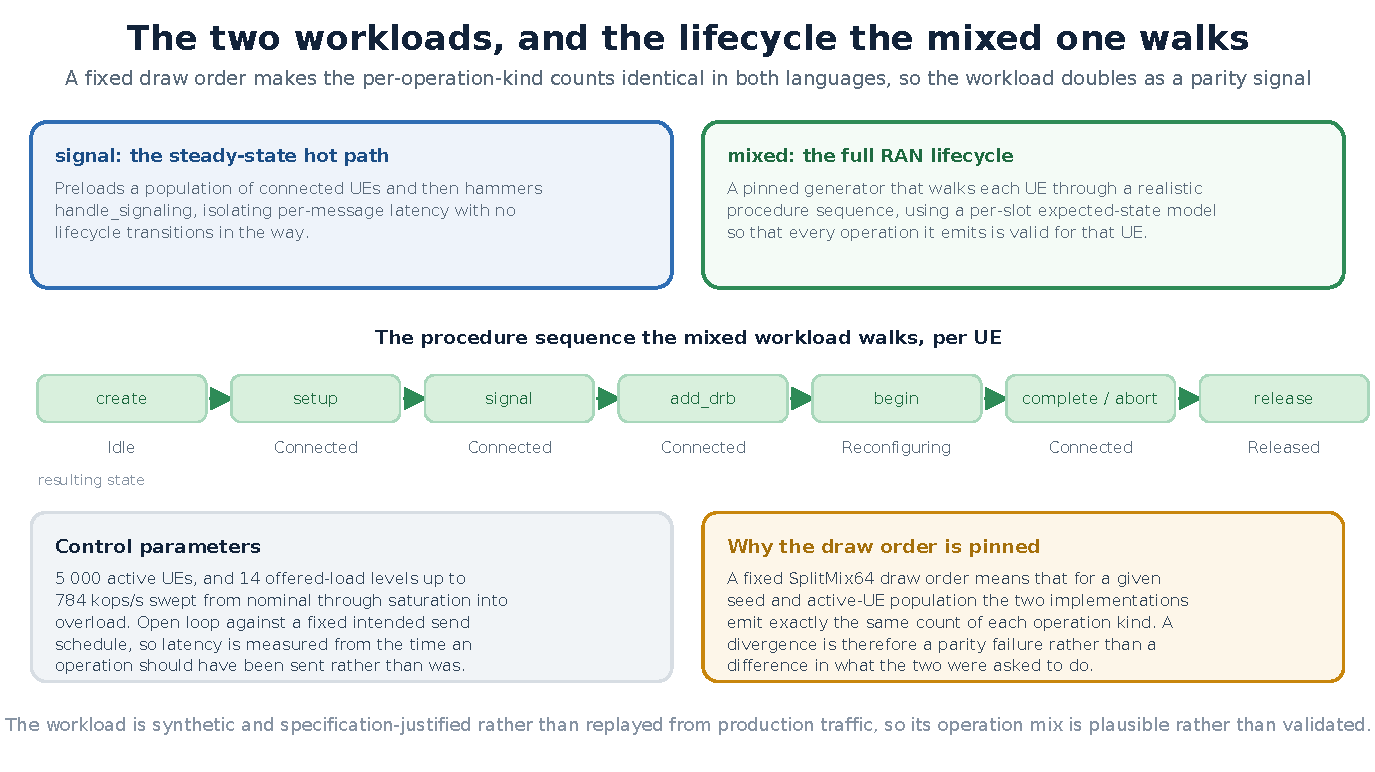
\includegraphics[width=\linewidth]{diagrams/pdf/27_workload_timeline.pdf}
\caption[The two workloads, and the lifecycle the mixed one walks]{The two workloads. The \emph{signal} workload isolates the steady-state hot path.
The \emph{mixed} workload walks each UE through the full RAN procedure sequence, with a
per-slot expected-state model ensuring that every operation it emits is legal for the state
its context is actually in. Because the SplitMix64 draw order is pinned, a given seed and
active-UE population produce identical per-operation-kind counts in both languages, so a
divergence is a parity failure rather than a difference in what the two implementations were
asked to do.\label{fig:workload}}
\end{figure}

\paragraph{What ``spec-justified'' claims, and what it does not.}
The term is used precisely, because the distinction bounds what the workload can support. The
\emph{sequence} of operations is justified: it is the RRC connection lifecycle the 3GPP
specifications define for a UE, from establishment through in-session signalling and bearer setup
to reconfiguration and release~\cite{3gpp38401,3gpp38331}, and the per-slot expected-state model
guarantees that every operation the driver emits is legal for the state its context is actually
in, so the workload never drives the service along a path the specification forbids. The
\emph{proportions} are not justified in the same way. How often a real cell hands over relative
to how often it establishes a bearer depends on deployment, mobility, and time of day, and no
public figure fixes it, so the mix used here is plausible rather than validated. That is
reported as a threat to external validity in Section~\ref{sec:threats}, and trace replay heads
the future-work list for exactly this reason.

For a \emph{comparative} question the distinction costs less than it would for an absolute one,
and saying why is part of arguing that the data suits the task. Both implementations execute the
same sequence in the same order for a given seed and active-UE population, verified through the
per-operation-kind counts, so an unrepresentative mix shifts both languages equally and cannot
manufacture a difference between them. An unvalidated operation mix therefore bounds how far the
numbers travel. It does not compromise the fairness of the comparison they are used to make.

Table~\ref{tab:params} gathers the configuration of all of this in one place. The values are
otherwise distributed across the specification, Chapter~\ref{chapter:design}, and this chapter,
which is convenient while reading each in turn and unhelpful to anyone trying to reproduce the
campaign or judge whether a parameter was chosen to suit the result. Every entry in the
campaign block is either fixed by the specification or generated from the measurement logs, so
the table cannot drift out of step with the data reported below.

\begin{table}
\centering
\small
\caption[Configuration of the service, the workload, and the campaign]{Configuration of the service under test, the workload driving it, and the measurement
campaign. Service parameters are fixed by the frozen specification, with one exception: the
shard count is set to match the cores the host offers (Section~\ref{sec:testbed}). All of them,
that one included, are identical in both languages. Campaign figures are generated from the
measurement logs together with the
tables that report them. The representative load is not chosen by eye but derived, as the
busiest swept load at which all four build variants still hold their p99 below
$5$~ms.\label{tab:params}}
\footnotesize
\renewcommand{\arraystretch}{1.05}
\begin{tabular}{@{}R{0.28\linewidth} R{0.28\linewidth} R{0.36\linewidth}@{}}
\hline\hline
Parameter & Value & Note \\
\hline
\multicolumn{3}{@{}l}{\emph{Service under test, identical in both languages}} \\
Shards, and worker threads & $7$ & one thread owns one shard, one of each per pinned core \\
Queue bound per shard & $1\,024$ requests & bounded and blocking, so overload is observable \\
Initial map capacity & $4\,096$ entries & reserved so steady state does not rehash \\
Bearers per context & at most $8$ & \\
Signaling payload & $64$ bytes & \\
Context ceiling per shard & $200\,000$ & \\
Shard selection & SplitMix64, then modulo & pinned: diffuses sequential identifiers \\
Intra-shard hash & FNV-1a, 64-bit & pinned on both sides and checked bit-for-bit \\
\hline
\multicolumn{3}{@{}l}{\emph{Workload}} \\
Workloads & signal, mixed & mixed walks the full RAN lifecycle \\
Active UEs & $5\,000$ & \\
Offered-load levels & \NLoadLevels{} & up to $\MaxOfferedLoad$~kops/s \\
Representative load & $\ReprLoad$~kops/s & derived, see caption \\
Measured saturation & $\SatKnee$~kops/s & tracks the offered rate to $\TrackingLoad$~kops/s \\
Load model & open loop, fixed intended schedule & latency measured from intended send time \\
\hline
\multicolumn{3}{@{}l}{\emph{Campaign}} \\
Build variants & $\NVariants$ & two languages $\times$ two allocators \\
Repeats per sweep point & \NRepeats{} & variants interleaved within each repeat \\
Measured runs & $\NRuns$ & \\
Latency capture & HDR histogram, $[1\,\text{ns}, 3.6\,\text{s}]$, 3 s.f. & same algorithm and configuration on both sides \\
Summary statistic & median with bootstrap $95\%$ CI & intervals reported in full, not as half-widths \\
Language comparison & exact paired permutation test & \NTests{} tests, Holm-corrected \\
Attainable $p$ floors & $\MinAttainableP$ / $\CorrectedFloor$ & uncorrected / after correction \\
\hline
\end{tabular}
\end{table}

\section{Evaluation data}
Three campaigns produce three datasets, and they differ in kind and not only in content. What
follows describes each as captured, because a reader judging whether the analysis is sound needs
to know what was recorded and at what granularity, not merely what was reported. No value is
hand-copied: \texttt{bench/refresh\_thesis.sh} regenerates every figure, table, and quoted number
directly from the raw logs, so the text and the data cannot drift apart. The software-quality
proxies are reported where they are most legible rather than gathered here, alongside the
forced-idiom log they explain (Table~\ref{tab:complexity}) and the FFI seam that is the only place
either implementation contains \texttt{unsafe} (Table~\ref{tab:ffi}).

\paragraph{The performance sweep.}
Each of the $\NRuns$ runs of the factorial design in Table~\ref{tab:params} contributes one
record, written as newline-delimited JSON so that a campaign is an append-only log rather than a
summary table: nothing is aggregated at capture time, and every statistic in this chapter is
recomputed from the raw records. A record carries the run's configuration (language, allocator,
workload, shard and producer counts, target rate), its outcome (operations completed, errors,
wall-clock duration, achieved throughput), the latency distribution read out of the HDR
histogram (mean, p50, p90, p99, p99.9, maximum, in nanoseconds), the resource counters taken
through \texttt{getrusage} (peak resident set size, user and system CPU seconds, CPU
utilisation), and the per-operation-kind counts. Retaining the kind counts in every record is
what makes a divergence between the two languages visible as a parity failure
(Section~\ref{sec:parity}) instead of being mistaken for a performance difference.

\paragraph{The component decomposition and contended primitives.}
The second measurement level of Section~\ref{sec:methodperf} yields a much smaller dataset of a
different shape: for each of \BudgetRepeats{} interleaved repeats, the batch-mean cost in both
languages of the operation called directly and of the same operation called through the threaded
service. A third dataset, of the same paired shape over \ContentionRepeats{} repeats, records
sustained throughput through the bounded queue and completion primitives alone
(Section~\ref{sec:contention}). The FFI comparison of Section~\ref{sec:migrationresults} has the
same structure over \FfiOpRepeats{} repeats. All three are paired by construction, which is what
the exact paired test of Section~\ref{sec:stats} requires.

\paragraph{The fault-injection catalogue.}
This dataset is categorical rather than numeric. Each of the ten defect cases yields four tool
logs, the AddressSanitizer, ThreadSanitizer and UndefinedBehaviorSanitizer output for the C++
program and the \texttt{rustc} output for the safe-Rust counterpart, together with one row in a
machine-readable taxonomy recording the three sanitiser outcomes, the detection stage, the
compiler result with the diagnostic codes that fired, and the expectation registered before the
study. The two original boundary cases yield a second table from the model checkers. Carrying the
expectation in the data instead of in the prose is what allows the runner to report a mismatch
in either direction. The table and figure in Section~\ref{sec:safetyresults} are generated from
that file, not transcribed from it.

\paragraph{What travels with the data.}
Every campaign writes an environment record beside its results, capturing host and kernel,
distribution, compiler and toolchain versions, CPU model and topology, and the frequency
governor, turbo, and simultaneous-multithreading settings, \emph{including} the fields a given
host does not expose. That detail matters more than it sounds. The record identifies the host as a
KVM guest, and the governor and turbo state are stored as unavailable rather than omitted, so the
limitation documented in Section~\ref{sec:testbed} is a property of the dataset itself and not only of the prose
describing it, and a reader can confirm the limitation without taking it on trust.

The performance dataset is complete and self-consistent as an analysis and is used below to
answer RQ1 and RQ3 provisionally. Rerunning the same scripts over a campaign captured on a
bare-metal host replaces these numbers with testbed-grade ones without any change to the
analysis.

\section{Evaluation results}
The safety and migration results do not depend on the measurement host at all. The performance and
resource results do, and Section~\ref{sec:testbed} states what that host can and cannot carry.
Every figure and table below is measured on it unless stated otherwise.

This chapter reports resolved and unresolved outcomes side by side. Which are which is worth
saying at the outset, so that a null result is not read as an absent one. Six findings are
resolved: the defect-class taxonomy and its boundary (Section~\ref{sec:safetyresults}), the cost
of the FFI seam (Section~\ref{sec:migrationresults}), the memory difference between the two builds
(Section~\ref{sec:resources}), the cost of the bare operation (Section~\ref{sec:budget}), the
equivalence of the four variants at the median below saturation, and their divergence past it
(Section~\ref{sec:overload}), which is the largest and most reproducible language effect in the
study.

One thing is unresolved, and one is resolved with a measured but inconclusive mechanism. The far
tail \emph{below} saturation is unresolved because of the host: run-to-run dispersion at p99
exceeds every difference between the variants, and no number of repeats on a virtualised machine
with non-zero CPU steal closes that gap (Section~\ref{sec:perfresults}). The overload divergence
is resolved as a measurement. Section~\ref{sec:contention} now tests whether the bounded queue and
completion primitives alone explain it, and finds they do not reproduce the full-service ordering
at significance. The bare-metal protocol of Section~\ref{sec:testbed} would answer the tail
question. What remains for the overload mechanism is work in the full handoff path beyond the
isolated primitives.

\subsection{Performance (RQ1, RQ3)}\label{sec:perfresults}
The hypothesis under test is H1: that the two languages are performance-equivalent below
saturation, with any difference confined to the far tail. This section reports where, if
anywhere, each wins and by how much, across the sweep up to and beyond saturation.

Everything in it, figures, tables, and the numbers quoted in the prose alike, is generated from
the raw logs by \texttt{bench/plot\_figures.py}, so the section can be regenerated verbatim if
the campaign is rerun on the bare-metal testbed. The absolute figures belong to the host of
Section~\ref{sec:testbed}. Each point aggregates \NRepeats{} interleaved repeats. Tabulated
values and shaded bands are medians with nonparametric bootstrap $95\%$ confidence intervals.

Table~\ref{tab:latency} summarises the per-operation latency distribution at a sustained
offered load of $\ReprLoad$~kops/s. That operating point is not chosen by eye: it is the
highest swept load at which every one of the four build variants still holds its p99 below
$5$~ms, that is, the busiest point at which all four are simultaneously healthy, which makes
it the fairest place to compare them.

The table must be read at two different levels of confidence, and separating them is the
honest reading of this campaign. At the \emph{median} the four variants sit within
$\PFiftyRange\,\mu$s of one another, or $\PFiftySpread\%$, and each variant's confidence
interval contains the others' point estimates, so the table on its own separates nothing.
That is a statement about unpaired intervals rather than about the languages: the paired test
below does resolve a small and consistent difference at the median, and the distance between
those two readings is precisely why Section~\ref{sec:stats} tests the comparison instead of
inspecting the intervals. \emph{Above} the median the situation is different in kind, and it
is not that the languages differ but that this host cannot say whether they do. The p99 values differ by
$\PNineNineRange\,\mu$s across variants, while the widest $95\%$ confidence interval on a
single variant's own p99 spans $\PNineNineMaxCI\,\mu$s, many times the between-variant
difference. When the uncertainty about one variant exceeds the gap between all of them, no
ordering can be read off, and reporting one would be reporting the scheduler. The same holds
with greater force at p99.9 and at the maximum.

This is the concrete form of the limitation stated in Section~\ref{sec:testbed}, and it is
worth being precise about what it does and does not cost. It does not affect the throughput
and saturation behaviour, the resource results below, or anything in the RQ2 and RQ4 chapters.
It does mean that one half of RQ1, how the two languages behave in the high percentiles while
the service is still meeting its offered load, is answered by this campaign only in the
negative: that tail is not yet measurable. It leaves the other half untouched. How they behave
once the service stops coping is resolved decisively on this same host, and
Section~\ref{sec:overload} reports it. Closing the remaining gap needs the bare-metal protocol and not more repeats on this
host, because the dispersion is systematic interference rather than sampling noise, and
Section~\ref{sec:budget} shows that the quantity a language could affect lies more than three
orders of magnitude below the one this measurement resolves.

One qualification about the metrics belongs here rather than only in the validity discussion.
RQ1 names the median, p99, p99.9, and the maximum, and it names those four because they are what
this campaign delivers. Two further statistics are instrumented but absent from it. The harness
records inter-operation jitter and p99.99, and persists the histograms the far tail would have to
be pooled from, but the campaign reported here predates that instrumentation. Predictability is
therefore evidenced at p99 and p99.9 rather than beyond them. That is a gap in the evidence rather
than in the design, and it closes with the same bare-metal campaign the tail claims already wait
on. Section~\ref{sec:threats} returns to what it costs the answer.

\begin{table}
\centering
\small
\caption[Per-operation latency at the representative load]{Per-operation latency at a sustained offered load of $\ReprLoad$~kops/s (mixed
RAN-lifecycle workload, $7$ shards). Values in microseconds: the median over \NRepeats{}
repeats above its nonparametric bootstrap $95\%$ confidence interval. The interval is printed
in full rather than as a symmetric half-width because it is strongly asymmetric at these
percentiles, and a half-width wide enough to cover the upper bound would place the lower one
below zero.\label{tab:latency}}
% Tabular preamble and header are generated alongside the table body, so the table
% gains a p99.99 column when a campaign records one instead of the preamble falling
% one column short of the body it is wrapping. \LatencyTabular expands to the whole
% \begin{tabular}{...}: array's preamble scanner does not expand macros, so passing
% only the column specification would fail with "Illegal pream-token".
\LatencyTabular
\hline\hline
\LatencyHead \\
\hline
C++ (system alloc) & \mci{217.2}{163.8}{237.2} & \mci{355.1}{289.3}{389.4} & \mci{674.3}{395.3}{1538.0} & \mci{2170}{910}{5594} \\
C++ (jemalloc) & \mci{225.8}{181.1}{261.2} & \mci{410.1}{305.7}{11280.4} & \mci{1188}{544}{14213} & \mci{3590}{1472}{16291} \\
Rust (system alloc) & \mci{214.3}{191.6}{238.8} & \mci{376.3}{330.2}{3629.1} & \mci{1068}{504}{6955} & \mci{2404}{1129}{9667} \\
Rust (jemalloc) & \mci{208.4}{193.7}{223.1} & \mci{388.9}{342.3}{478.0} & \mci{763.4}{479.5}{4272.1} & \mci{2804}{1114}{7606}
\\
\hline
\end{tabular}
\end{table}

\paragraph{Testing the comparison rather than eyeballing it.}
Overlapping intervals are a weak instrument in both directions, so the comparison is also tested
directly, by the procedure fixed in Section~\ref{sec:stats} and reported in
Table~\ref{tab:significance}. What licenses the pairing is a property of this campaign and
not of the statistic: because the four variants are interleaved inside every repeat, the
$i$-th run of each was measured in the same block under the same ambient conditions, so the
interference that block carried is common to the pair and cancels in their difference. That is
the second thing the interleaving discipline buys, beyond the fairness argument it was adopted
for.

\begin{table}
\centering
\small
\caption[Exact paired permutation test of C++ against Rust]{Exact paired permutation test of C++ against Rust at $\ReprLoad$~kops/s, with the
allocator held fixed. The effect is the median of the \NRepeats{} paired differences
(Rust~$-$~C++), shown above its bootstrap $95\%$ confidence interval. The test statistic is
their mean. $p$ is exact over all $2^{\NRepeats}$ sign assignments, and the final column
applies the Holm correction across the whole family of \NTests{} tests. The attainable floors
are $\MinAttainableP$ uncorrected and $\CorrectedFloor$ after correction. The rows are blocked
by the criterion set out in Section~\ref{sec:stats}: pairing rescues the statistics in the
upper block, so a consistent interval there is evidence, whereas the high percentiles below are
computed from exactly the operations interference falls on, so an interval excluding zero is
not read as a finding. Achieved throughput is not tested, for the reason given in the same
section, and appears in Table~\ref{tab:resource} instead. Measured on the virtualised Xeon host
of Section~\ref{sec:testbed}.\label{tab:significance}}
\begin{tabular}{@{}l l r r r@{}}
\hline\hline
Metric & Allocator & Effect (Rust $-$ C++) & $p$ & Holm \\
\hline
\rlap{\emph{Robust to interference on single operations}} & & & & \\
p50 latency (\textmu s) & system & \mci{-1.3}{-1.3}{-1.2} & 0.0000019 & 0.000027 \\
p50 latency (\textmu s) & jemalloc & \mci{-1.2}{-1.3}{-1.2} & 0.0000019 & 0.000027 \\
Peak RSS (MiB) & system & \mci{+1.4}{+1.2}{+1.7} & 0.0000019 & 0.000027 \\
Peak RSS (MiB) & jemalloc & \mci{+2.5}{+2.4}{+2.6} & 0.0000019 & 0.000027 \\
CPU utilisation (\%) & system & \mci{-5.1}{-6.7}{-4.7} & 0.0000019 & 0.000027 \\
CPU utilisation (\%) & jemalloc & \mci{-4.6}{-5.9}{-3.9} & 0.0000019 & 0.000027\\
\hline
\rlap{\emph{Determined by it: high percentiles}} & & & & \\
p99 latency (\textmu s) & system & \mci{-1}{-2}{-1} & 0.0000057 & 0.000027 \\
p99 latency (\textmu s) & jemalloc & \mci{-1}{-1}{-1} & 0.0000038 & 0.000027 \\
p99.9 latency (\textmu s) & system & \mci{-4}{-5}{-2} & 0.00016 & 0.00016 \\
p99.9 latency (\textmu s) & jemalloc & \mci{-2}{-4}{-2} & 0.0000095 & 0.000027
\\
\hline
\end{tabular}
\end{table}

\begin{figure}
\centering
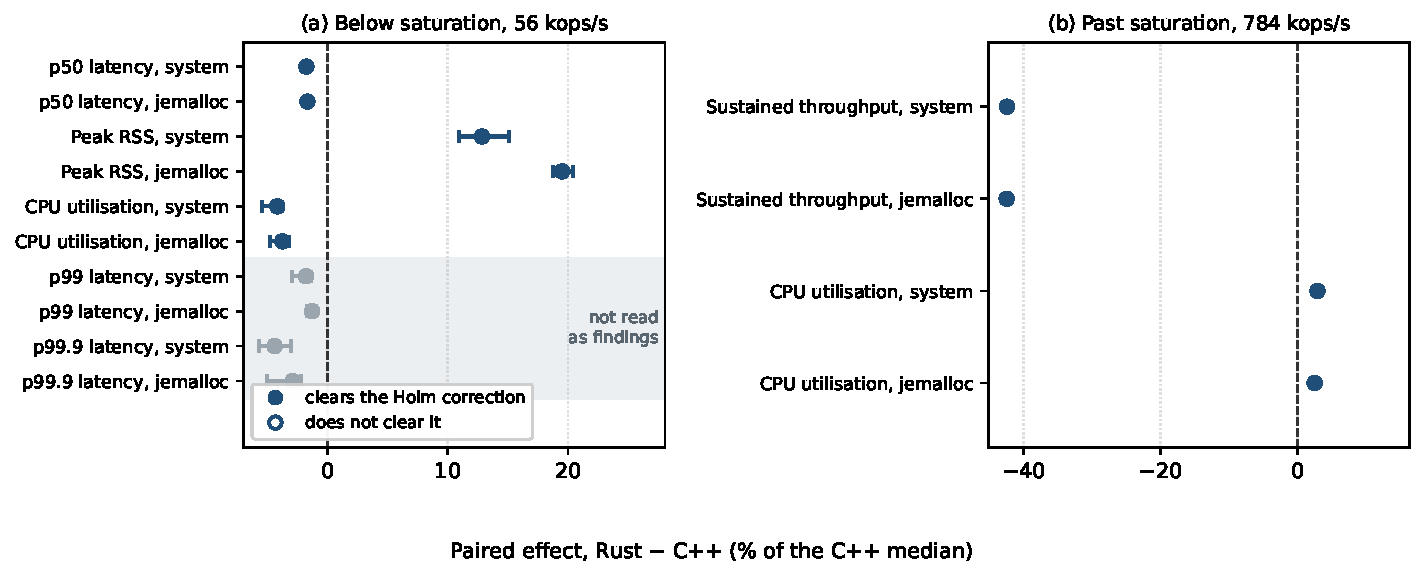
\includegraphics[width=\linewidth]{figures/fig_effects.pdf}
\caption[The tested family drawn as paired effects]{Every test in Tables~\ref{tab:significance} and~\ref{tab:overloadtest} as a paired
effect with its bootstrap $95\%$ interval, normalised by the C++ median so that microseconds,
mebibytes, percentage points and kops/s can share an axis. Filled markers are the
\NSignificant{} of \NTests{} tests that clear the Holm correction. The two allocators of a
metric are drawn adjacent, so an effect that reversed sign between them would appear as a pair
straddling the zero line. The shaded rows are the high percentiles, computed from exactly the
operations interference falls on, which Section~\ref{sec:stats} fixes in advance as rows whose
intervals are not read as findings. The metrics keep their own units in the
tables.\label{fig:effects}}
\end{figure}

Figure~\ref{fig:effects} draws the same family on one axis, and three things it contains are
easier to see there than in a table of fourteen rows: which effects survive the correction,
whether an effect keeps its sign when the allocator changes, and how much wider the tail
intervals are than the rest.

Four things follow. First, \NSignificant{} of the \NTests{} tests in the family survive the Holm
correction. At this operating point they are the two median-latency rows, peak resident set size
under the system allocator, and both CPU rows. The four remaining survivors are the overload
comparisons of Section~\ref{sec:overload}. Peak resident set size under jemalloc is the one
robust-block row that does not clear the correction despite an interval nowhere near zero, and
Section~\ref{sec:resources} takes up why.

Second, the reading rule fixed in Section~\ref{sec:stats} has to be applied before those are
interpreted. \NExclZero{} paired intervals exclude zero. In the tail block the intervals that do
so are: \TailExclZeroRows. The rule is stated in advance rather than at this point precisely
because that outcome is not guaranteed, and an earlier seven-repeat pass of the same campaign did
produce tail intervals excluding zero which more repeats then removed, which is the behaviour the
rule anticipates.

Third, the allocator control supplies a second and independent check: every comparison is run
twice under conditions that should not change a language effect, so an effect that is genuinely
the language ought to keep its sign whichever allocator is linked. Here
\CrossAllocConsistent{} all do, and \NCrossAllocReversed{} reverse. That the control confirms
rather than vetoes is not evidence that it was unnecessary: on an earlier campaign, run before the
two \texttt{jemalloc} builds were held to one configuration, the CPU effect cleared the correction
under one allocator and reversed sign under the other, and was reported as unresolved on exactly
this rule. A control is worth keeping because of what it would have caught, not because of what
it happens to catch.

Fourth, the median, which is now a resolved difference rather than a null: $\PFiftyDiffAbsMax\,\mu$s
in Rust's favour, consistent under both allocators. The interval on it reaches
$\PFiftyDiffCIMax\,\mu$s against a median of roughly $80\,\mu$s, and the temptation is to report
that as a bound on the language effect. That reading would be wrong, and the reason is the
subject of the next section.

\subsection{What the end-to-end number is made of}\label{sec:budget}
Every latency the sweep reports is an end-to-end round-trip, and
Section~\ref{sec:methodperf} set out why that bundles two costs of quite different character:
the operation itself, executed inside one thread and generated by the compiler, and the
cross-thread submit-and-complete handoff around it, charged to the operating system. Only the
first can plausibly differ between the languages, and the sweep cannot separate them.

That matters for the bound just quoted, because a bound is only as informative as the quantity
it is a fraction of. The two are therefore measured directly by the two-level method described
there, in both languages and at the sweep's own shard count and context population:
\texttt{ShardCore} called with no queue in the path gives the operation, \texttt{Service} gives
the operation plus the handoff, and their difference is the handoff.
Table~\ref{tab:budget} gives the result, and it reframes the whole performance comparison.

\begin{table}
\centering
\small
\caption[Where an end-to-end operation's cost actually goes]{Where an end-to-end operation's cost actually goes, measured at $7$ shards and
$5\,000$ active UEs with a single uncontended caller. Each row is the median over
\BudgetRepeats{} interleaved repeats above its bootstrap $95\%$ confidence interval, in the
unit its own magnitude calls for: the two terms differ by more than two orders of magnitude,
which is the point of the table. $p$ is the exact two-sided paired permutation test of C++
against Rust on the repeat-wise differences. The handoff is obtained as the difference between
the two measured rows, so it carries the uncertainty of both.\label{tab:budget}}
\begin{tabular}{@{}l r r r@{}}
\hline\hline
Component & C++ & Rust & $p$ \\
\hline
Operation alone, no queue in the path (ns) & \mci{34.4}{32.5}{34.5} & \mci{21.3}{21.0}{22.5} & 0.000061 \\
Cross-thread submit-and-complete handoff (\textmu s) & \mci{13.49}{13.36}{13.64} & \mci{12.61}{12.37}{12.89} & 0.227 \\
End-to-end round-trip, uncontended (\textmu s) & \mci{13.52}{13.39}{13.68} & \mci{12.63}{12.39}{12.91} & 0.215 \\
Operation's share of the round-trip & 0.250\,\% & 0.170\,\% & 
\\
\hline
\end{tabular}
\end{table}

The operation is $\BudgetCoreCpp$~ns in C++ and $\BudgetCoreRust$~ns in Rust. The handoff is
$\BudgetHandoffCpp\,\mu$s and $\BudgetHandoffRust\,\mu$s. The work the languages actually
perform is therefore at most $\BudgetCoreShareMax\%$ of what the sweep measures, and better
than $99.9\%$ of every latency in Table~\ref{tab:latency} is the operating system moving a
message between two threads.

That shape is not peculiar to this system or to this pair of languages. Revisiting a classic
decomposition of transaction-processing cost on a shared-nothing database structured, as this
service is, with one partition per worker thread, Zhou et al.\ report that once the
per-operation work has been optimised the remaining cost is dominated by communication across
isolation boundaries and not by the operation itself~\cite{zhou2025oltp}. A mature
shared-nothing design tends to end up communication- and scheduler-bound, and the table above is
that pattern appearing in a control-plane service. It is worth saying because it makes the result
below a general property of the design rather than an artefact of this measurement.

Two conclusions follow, and they pull in opposite directions.

The first is that the sweep cannot bound the language effect, and the bound quoted above should
not be read as though it does. An interval of $\PFiftyDiffCIMax\,\mu$s on the paired median
difference is $\BudgetBoundVsCore$ times the operation's own cost. A language effect could be
several hundred percent of the work being done and sit comfortably inside it. What the sweep
establishes is the much weaker and still useful statement that neither language perturbs the
scheduler-dominated round-trip, which is what a deployment of this shape would actually
experience. What it cannot establish, at any repeat count, is anything about the code the
compilers emit. That is a property of the measurement's construction rather than of the host,
so unlike the tail result it will not be fixed by moving to bare metal. It is fixed by
measuring the component separately, which is what this section does.

The second is that once the component \emph{is} measured separately, the languages are not
equivalent. \BudgetCoreFaster{} runs the bare operation about $\BudgetCoreRatio\times$ faster,
the difference is present in the great majority of repeats, and the paired test puts it two
orders of magnitude below the conventional threshold. This decomposition is a separate
experiment from the sweep and is not part of its Holm family: it runs \BudgetRepeats{} repeats
instead of \NRepeats{}, so its own attainable floor is $0.000061$ rather than the
$\CorrectedFloor$ quoted in Section~\ref{sec:stats}, and no correction is applied to it. The
same holds for the interoperability comparison of Section~\ref{sec:migrationresults}. This is
the only place in the whole performance campaign where a
language difference in \emph{time} is resolved at all, and the sweep is blind to it by more
than two orders of magnitude.

Figure~\ref{fig:budget} draws both conclusions on one page, because each is easier to see than
to read off a table of numbers spanning four decades. The left panel is the round-trip at true
proportion, where the operation is a sliver too thin to render and the caption has to point at
it. The right panel puts that sliver on a log axis beside the smallest paired difference the
sweep could have detected, and the ordering there is the argument of this section: the
instrument sits entirely above the quantity it would have to constrain.

\begin{figure}
\centering
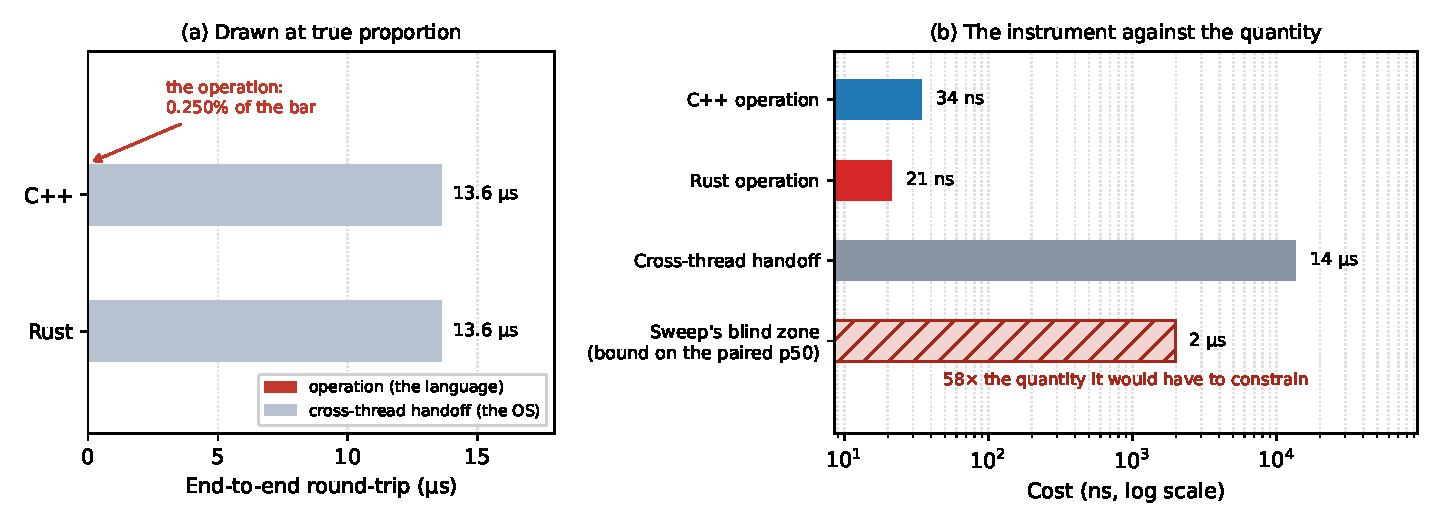
\includegraphics[width=\linewidth]{figures/fig_budget.pdf}
\caption[The end-to-end operation decomposed, against what the sweep can resolve]{Where an end-to-end operation's cost goes, and why the sweep cannot bound a language
effect. \textbf{(a)} The round-trip at true proportion: the operation the language performs is
$\BudgetCoreShareMax\%$ of the bar, the remainder the cross-thread handoff. \textbf{(b)} The
same quantities on a log axis against the smallest paired difference the sweep can resolve,
shown as a blind zone. Both operation measurements fall inside it by a factor of
$\BudgetBoundVsCore$, and (b) is also where the campaign's one resolved timing difference
lives.\label{fig:budget}}
\end{figure}

The attribution deserves care, because the obvious reading is the wrong one. Nothing here
implicates the borrow checker, bounds checking, or ownership. The single most likely source is
already recorded in the forced-idiom log of Table~\ref{tab:idioms}: the per-shard container is
each language's standard hash map, and those are different data structures. C++'s
\texttt{std::unordered\_map} is required by its iterator- and reference-stability guarantees to
be node-based, so a lookup chases a pointer out of the bucket array into a separately allocated
node, whereas Rust's \texttt{HashMap} is an open-addressed table that keeps entries inline and
usually resolves a lookup within one cache line. The hash function is pinned to FNV-1a on both
sides (Section~\ref{sec:impldetails}) precisely so that hashing could not be the explanation,
which leaves the container layout. That is a real and reportable difference between the two
languages as they are actually used, since a developer reaching for the standard hash map gets
whichever one their language ships. It is not evidence about Rust's safety model, and it should
not be quoted as such. Confirming the mechanism would need the cache-miss counters
Section~\ref{sec:threats} lists as the clearest instrumentation gap.

Three limits keep the finding the size it is. It is a single-threaded, uncontended
microbenchmark, so it says what the operation costs and not what a loaded system does with it.
It is measured on the same host as the sweep, so the absolute figures carry the
same caveat, although the ratio is far more robust than either term. And it is one operation on
one data structure: generalising from it to ``Rust is $\BudgetCoreRatio\times$ faster'' would repeat exactly the
error this thesis criticises in the average-case literature.

\subsection{Latency, throughput, and saturation across the sweep}
Figure~\ref{fig:latency-load} plots p99 latency against offered load, and the shape it shows is
the one Figure~\ref{fig:cliff} sketched. Through the tracking region the four variants climb
together and gently, from roughly $240\,\mu$s at the lightest load to single-digit milliseconds
by $\SatKnee$~kops/s, with confidence bands wide enough that no curve can be separated from
another anywhere in that region. Then, in the single step of the rate ladder that follows, every
variant's p99 rises by more than two orders of magnitude at once, from about $6$~ms to several
seconds. That is the overload cliff, and the sharpness of its onset is the finding: one increment
of offered load separates a service meeting millisecond deadlines from one missing them by three
orders of magnitude. A design with bounded, blocking queues has no graceful degradation to offer
in between.

Two properties of the far side of the cliff bound what those numbers mean, and they are the
reason Section~\ref{sec:stats} tests no percentile there: latency past the knee is accumulated
schedule backlog rather than service time, and because the measured phase is truncated the
reported percentiles saturate near the width of that window, which makes every one of them
above the knee a lower bound. What remains interpretable in this regime is how much work each
variant still completes, and Section~\ref{sec:overload} takes that up.

\begin{figure}
\centering
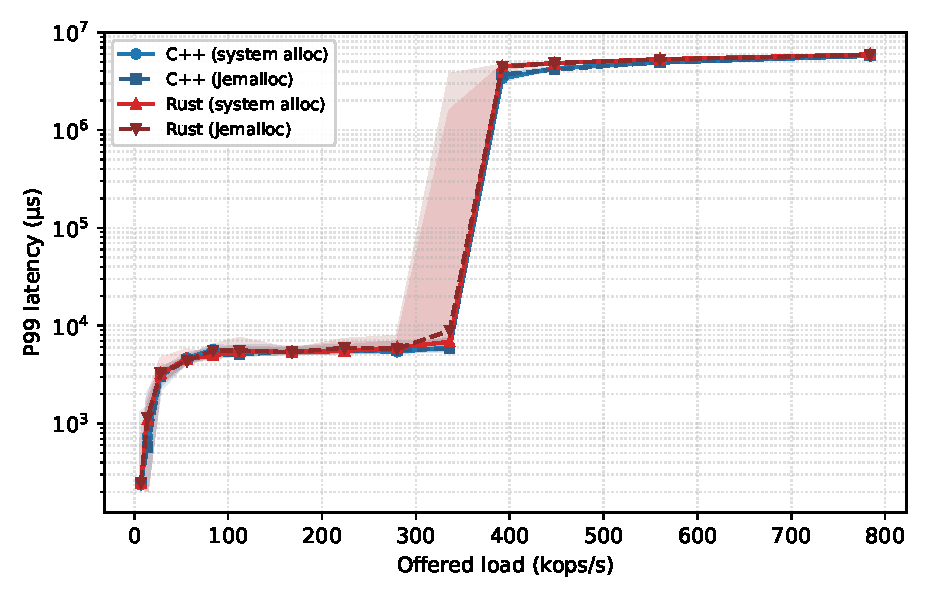
\includegraphics[width=0.82\linewidth]{figures/fig_latency_vs_load.pdf}
\caption[Tail latency versus offered load]{Tail latency (p99) versus offered load for the four build variants. Lines are medians
over \NRepeats{} repeats. Shaded bands are bootstrap $95\%$ CIs. Log-scaled $y$-axis.
\label{fig:latency-load}}
\end{figure}

Figure~\ref{fig:throughput-load} shows achieved throughput against offered load, and it is the
more informative of the two plots, because throughput is an average over a whole run and
therefore far more robust than a percentile to interference landing on individual operations.
Every variant tracks the ideal offered-equals-achieved line up to $\TrackingLoad$~kops/s and
saturates at around $\SatKnee$~kops/s. Two things follow immediately. First, because achieved
throughput matches offered load below the knee to within $\ReprLoadShortfall\%$, the operating
point of Table~\ref{tab:latency} is genuinely a \emph{sustained} load rather than a nominal one:
the system is completing work as fast as it is offered, so the latencies reported there are not
those of an already-queueing system. Second, the knee itself sits at the same place for all four
variants, which is what the identical thread-per-shard structure predicts: where the design stops
coping is a property of the design.

What happens \emph{after} the knee is not shared. The four curves separate as soon as the
offered rate stops being met, and they separate by language rather than by allocator, which is
the one thing the sweep was built to be able to detect and the one regime in which it can.
Section~\ref{sec:overload} measures that separation instead of leaving it to the eye.

\begin{figure}
\centering
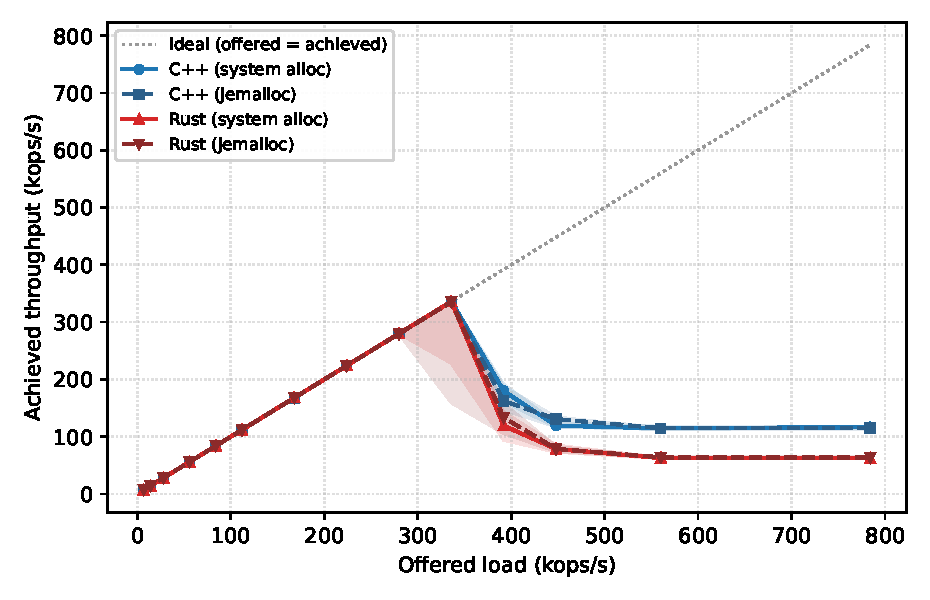
\includegraphics[width=0.82\linewidth]{figures/fig_throughput_vs_load.pdf}
\caption[Achieved throughput versus offered load]{Achieved throughput versus offered load. The dotted line marks the ideal
offered-equals-achieved regime. Throughput is counted over the measured phase only, so the
warm-up iterations bias neither the numerator nor the denominator.\label{fig:throughput-load}}
\end{figure}

Figure~\ref{fig:tailpct} holds the load fixed instead and sweeps the percentile. The four
variants coincide at the median and fan out as the percentile rises, which is the expected shape
for a heavy-tailed distribution and is why a percentile-aware methodology is used throughout. The
fanning is not a language effect, and the right-hand panel is the reason. It sets the spread
between the four variants at each percentile against the widest interval any single variant
carries there. At the median the spread is the larger of the two quantities, which is the regime
in which an ordering means something. From p90 upward the interval exceeds the spread several
times over, so the fan marks where the measurement loses resolution rather than where the
languages differ.

\begin{figure}
\centering
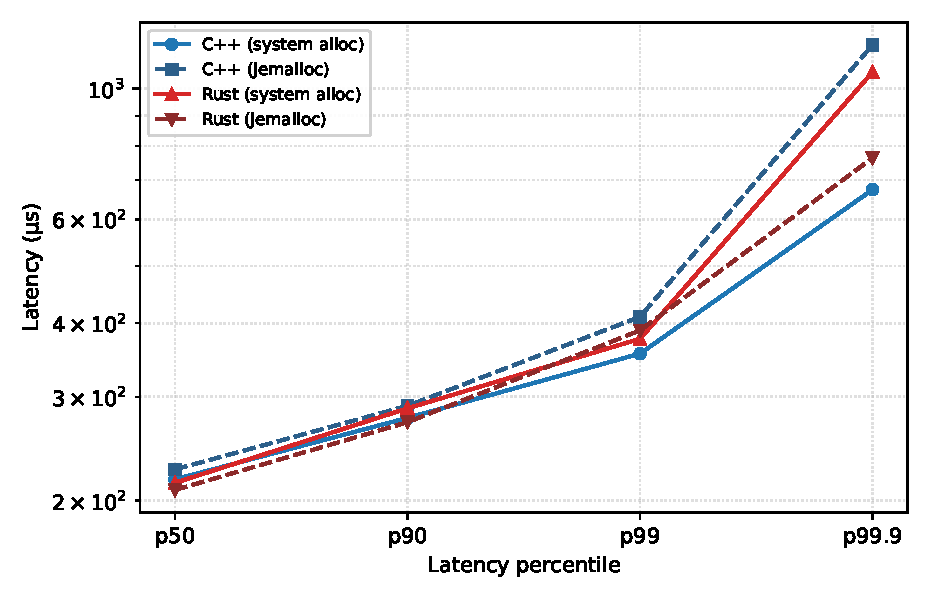
\includegraphics[width=\linewidth]{figures/fig_tail_percentiles.pdf}
\caption[Latency across the percentile range, and the limit of the host]{Per-operation latency across the percentile range at $\ReprLoad$~kops/s. \textbf{(a)} The
four variants as medians over \NRepeats{} repeats, each with a bootstrap $95\%$ band. The bands
are the point: drawn as bare lines the curves lie on top of one another and read as a claim of
equivalence, which is not what a measurement that cannot separate them has shown. \textbf{(b)}
Why they cannot be separated above the median. The spread between the four variants is set
against the widest confidence interval on any one of them, with the ratio annotated above each
pair of bars. Once that ratio passes one, the uncertainty about a single variant is larger than
the gap between all four and no ordering can be read off.\label{fig:tailpct}}
\end{figure}

\subsection{Behaviour past saturation (RQ1)}\label{sec:overload}
RQ1 asks how the two languages compare under increasing load \emph{and overload}, and everything
reported so far has been below the knee. This section is the other half. The operating point is
$\OverloadLoad$~kops/s offered, defined as the deepest swept load at which every variant has
stopped meeting the offered rate, and the metrics are the two that remain interpretable there
(Section~\ref{sec:stats}). Table~\ref{tab:overload} gives what each variant still sustains and
Table~\ref{tab:overloadtest} tests the comparison.

The languages are not equivalent in this regime, and the margin is not marginal.
\OverloadSustainedFaster{} sustains $\OverloadThrCpp$~kops/s where \OverloadSustainedSlower{}
sustains $\OverloadThrRust$, a factor of $\OverloadThrRatio$. The paired difference is at least
$\OverloadThrBound$~kops/s under either allocator, it holds in \OverloadThrAgree{} repeats, and
its Holm-adjusted $p$ sits at the corrected floor of the whole family of \NTests{} tests. This is
the largest and most reproducible language effect anywhere in the study, and it is the only one
that speaks directly to the question RQ1 was written to ask.

The CPU column is what makes the result interpretable rather than merely large, because it rules
out the reading that would otherwise be natural. A variant that completes less work might simply
be doing less: throttled, blocked, idle. That is not what happens.
\OverloadSustainedSlower{} draws \emph{more} total CPU than \OverloadSustainedFaster{} here,
reproducibly and under both allocators, having inverted the sign it carried at the representative
load in Table~\ref{tab:significance}. Divided through by the work that actually completed, its
CPU cost per sustained operation is $\OverloadCpuPerOpRatio$ times the other's. Nor is either
variant near the capacity of the machine: both sit near six of the fourteen pinned cores. So the
gap is not a capacity limit and not idleness. It is effort expended without completing
operations, which is the signature of a synchronisation path that spins, or repeatedly parks and
wakes, where the other blocks once and sleeps.

Figure~\ref{fig:overload} puts both halves of that reading side by side, and its layout carries a
third. The bars are grouped by allocator, so the separation inside a group is the language and
the separation between groups is the allocator. It falls almost entirely inside the groups, which
is the effect following the variable the study manipulates rather than the one it controls for.

\begin{figure}
\centering
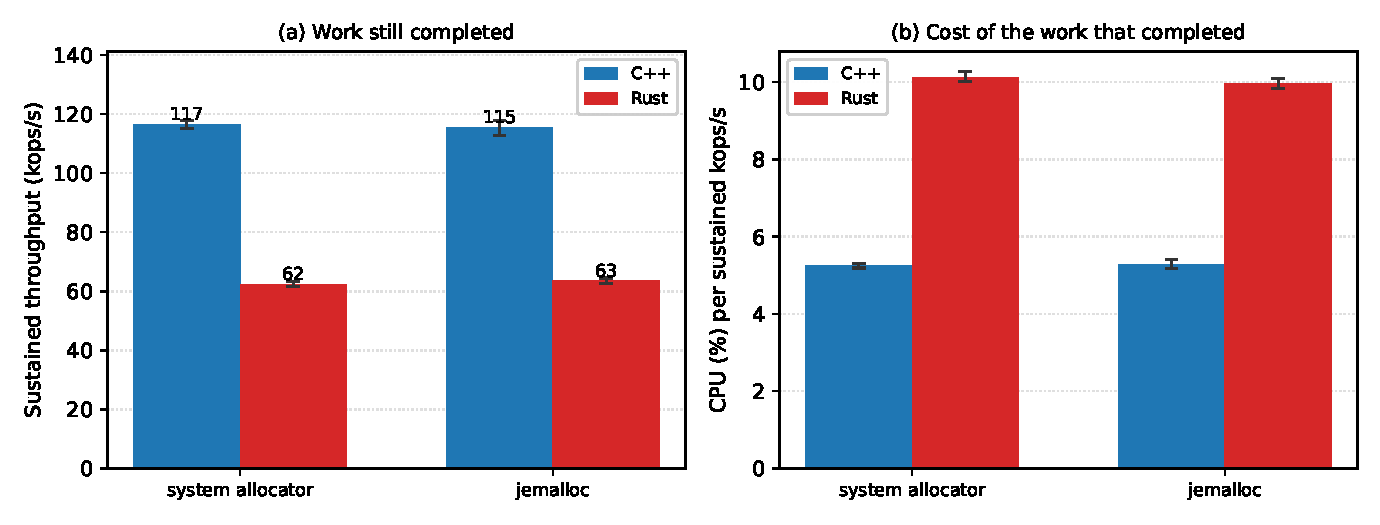
\includegraphics[width=\linewidth]{figures/fig_overload.pdf}
\caption[Divergence past saturation]{Behaviour at $\OverloadLoad$~kops/s offered, well beyond the $\SatKnee$~kops/s knee. Bars
are medians over \NRepeats{} repeats with bootstrap $95\%$ intervals, grouped so that the two
bars inside a group differ only in language. \textbf{(a)} What each variant still completes:
\OverloadSustainedFaster{} sustains a factor of $\OverloadThrRatio$ more than
\OverloadSustainedSlower. \textbf{(b)} Total CPU divided by the work that actually completed,
which is what rules out the reading that the variant delivering less is simply doing less. It
spends $\OverloadCpuPerOpRatio$ times as much CPU per sustained operation, and the CPU figures
are summed across threads.\label{fig:overload}}
\end{figure}

Where that effort is spent is narrowed by measurement rather than left entirely open. Past
saturation the producers spend essentially all of their time in two places recorded in
Table~\ref{tab:idioms}: the bounded blocking queue and the completion handle. Section~\ref{sec:contention}
isolates those primitives under the same seven-producer pattern. The isolated path does not
reproduce the full-service ordering at significance ($p = \ContentionP$), which rules out the
queue and completion primitives \emph{alone} as the whole explanation for a
$\OverloadThrRatio\times$ gap even though contention in the full path is where the effect appears.
Nothing in the borrow checker, in bounds checking, or in ownership is implicated, and the finding
should not be quoted as though it were: what the overload comparison measures is the full
handoff under load, and the microbenchmark shows the synchronisation stacks are closer than that
comparison alone would suggest.

Three things again bound what the finding licenses. It is one design: a shared-nothing service with one
request outstanding per producer and a queue bound of $1\,024$, and the depth of the collapse
depends on all three. It is measured with a harness whose producers block per request, so it
describes what this shape of client experiences rather than what a pipelined one would.
And the absolute figures belong to this host. What travels is the ordering and its cause: below
saturation the language choice did not matter, above it the standard library's synchronisation
primitives did, and the crossover is sharp enough that a comparison stopping at nominal load
would have concluded the opposite.

That crossover also bears on the closest prior work, which reports a comparable degradation past
a threshold request rate and attributes it to the asynchronous
runtime~\cite{arvidsson2025async}. Section~\ref{sec:rqdiscussion} takes up what it means that the
same shape appeared here with no such runtime on either side.

\begin{table}
\centering
\small
\caption[What each variant sustains past saturation]{What each variant still sustains at
$\OverloadLoad$~kops/s offered, well beyond the $\SatKnee$~kops/s knee: the median over
\NRepeats{} repeats above its bootstrap $95\%$ confidence interval. Below saturation achieved
throughput is pinned to the offered rate by construction and can express nothing about the
languages. Here it is the only thing that can. CPU utilisation exceeds $100\%$ because it is
summed across threads, so $600\%$ is six busy cores of the fourteen
pinned.\label{tab:overload}}
\begin{tabular}{@{}l r r@{}}
\hline\hline
Variant & sustained throughput (kops/s) & CPU (\%) \\
\hline
C++ (system alloc) & \mci{146.7}{146.3}{147.2} & \mci{662.8}{662.5}{663.6} \\
C++ (jemalloc) & \mci{146.4}{146.1}{146.9} & \mci{664.3}{663.3}{664.9} \\
Rust (system alloc) & \mci{84.5}{84.2}{84.7} & \mci{681.8}{680.4}{682.5} \\
Rust (jemalloc) & \mci{84.3}{83.9}{84.6} & \mci{680.3}{679.8}{681.5}
\\
\hline
\end{tabular}
\end{table}

\begin{table}
\centering
\small
\caption[Exact paired test past saturation]{Exact paired permutation test of C++ against Rust at
$\OverloadLoad$~kops/s, the allocator held fixed, Holm-corrected across the same family of
\NTests{} tests as Table~\ref{tab:significance} rather than as a family of its own. ``Repeats''
counts how many of the \NRepeats{} paired differences agree with the sign of the median, which a
statistic computed from their mean cannot show. No latency percentile is tested here, for the
reason fixed in advance in Section~\ref{sec:stats}.\label{tab:overloadtest}}
% The generated metric names are long enough that six l/r columns overrun the text
% block; the first column wraps instead, and the inter-column padding is tightened.
\setlength{\tabcolsep}{4pt}
\begin{tabular}{@{}p{0.24\linewidth} l r c r r@{}}
\hline\hline
Metric & Allocator & Effect (Rust $-$ C++) & Repeats & $p$ & Holm \\
\hline
Sustained throughput (kops/s) & system & \mci{-62.2}{-62.9}{-61.6} & 20/20 & 0.0000019 & 0.000027 \\
Sustained throughput (kops/s) & jemalloc & \mci{-62.2}{-62.7}{-61.6} & 20/20 & 0.0000019 & 0.000027 \\
CPU utilisation (\%) & system & \mci{+19.5}{+17.3}{+19.9} & 20/20 & 0.0000019 & 0.000027 \\
CPU utilisation (\%) & jemalloc & \mci{+16.8}{+15.6}{+17.5} & 20/20 & 0.0000019 & 0.000027
\\
\hline
\end{tabular}
\end{table}

\subsection{Contended queue and completion primitives (RQ1)}\label{sec:contention}
The overload result attributes its gap to the two forced-idiom synchronisation constructs, but
that attribution was argued from the shape of the full-service measurement. This subsection
isolates those constructs alone.

Seven producer threads hammer one bounded queue of capacity $1\,024$ while a single consumer
drains it. Each producer submits a no-op job carrying a one-shot completion handle and blocks
until the consumer signals. No \texttt{ShardCore} work runs in the path. C++ uses the
hand-written \texttt{BoundedQueue} of Section~\ref{sec:impldetails} with
\texttt{std::promise}/\texttt{std::future}. Rust uses \texttt{sync\_channel} and a fresh
\texttt{mpsc::channel()} per request. Each timed window lasts two seconds after a warmup.
\ContentionRepeats{} interleaved repeats are summarised as medians with bootstrap intervals and
tested with the exact paired permutation procedure of Section~\ref{sec:stats}.
Table~\ref{tab:contention} reports the result.

\begin{table}
\centering
\small
\caption[Throughput through the contended synchronisation primitives alone]{Throughput through
the bounded queue and completion primitives alone, with seven contending producers and queue
capacity $1\,024$. Values are medians over \ContentionRepeats{} interleaved repeats above
bootstrap $95\%$ confidence intervals. The paired test compares C++ against Rust on sustained
throughput (kops/s). Measured on the host of Section~\ref{sec:testbed}.\label{tab:contention}}
\begin{tabular}{@{}l r r r@{}}
\hline\hline
Language & Throughput (kops/s) & Mean ns/op & Paired $p$ \\
\hline
C++ & \mci{55.0}{53.7}{58.4} & \mci{18178}{17110}{18632} & \multicolumn{1}{c}{---} \\
Rust & \mci{58.7}{56.8}{61.8} & \mci{17045}{16169}{17594} & 0.226
\\
\hline
\end{tabular}
\end{table}

The isolated primitives do not reproduce the overload ordering. C++ sustains
\ContentionThrCpp{}~kops/s and Rust \ContentionThrRust{}~kops/s, a gap of only
$\ContentionRatio\times$ with $p = \ContentionP$, whereas the full service at
$\OverloadLoad$~kops/s separates by $\OverloadThrRatio\times$ with the corrected $p$ at the
family floor. The honest reading is therefore that the overload divergence involves additional
work the microbenchmark strips away: the larger tagged \texttt{Request} on the C++ side, the
worker's variant dispatch, and the map operations that still execute in the overload regime.
What the result still establishes is useful: an orders-of-magnitude difference in the primitives
alone is ruled out, and the search for the mechanism moves to the rest of the handoff path rather
than to the safety model.

\subsection{Resource use (RQ3)}\label{sec:resources}
Table~\ref{tab:resource} reports resource use at the same
sustained load. Peak resident set size separates the four variants cleanly, and it does so
whichever way the family is read: its intervals exclude zero, and its effect keeps its sign under
both allocators. Figure~\ref{fig:resources} plots the same measurement, and its middle panel is
where the finding of this section sits, with the two effects inside peak RSS measured as paired
differences on a shared axis.

Two effects are present in it, not one, and they are not of comparable size. Linking
\texttt{jemalloc} costs $\RssAllocDiffLo$--$\RssAllocDiffHi$~MiB in either language, while the Rust
build costs $\RssLangDiffLo$--$\RssLangDiffHi$~MiB more than the C++ build under either allocator,
with a bootstrap interval of $\RssLangCILo$ to $\RssLangCIHi$~MiB. So resource use follows both,
but the allocator dominates by an order of magnitude: choosing between these two allocators moves
roughly ten times as much memory as choosing between these two languages. That ordering is partly
a consequence of the fairness controls rather than a fact about \texttt{jemalloc} in general, and
saying so avoids overstating it. Both builds pin the arena count identically so that neither
language's default could become an accidental advantage, and pinning it high is what makes the
arena metadata a large fixed cost on both sides. A deployment tuning \texttt{jemalloc} for
footprint instead of for comparability would not pay it.

The one row in the robust block of Table~\ref{tab:significance} that does not clear the
correction is peak RSS under
\texttt{jemalloc}, and the reason is a property of the statistic rather than of the software. The
interval there is tight, nowhere near zero, and $18$ of the $20$ paired repeats agree. What
defeats the test is a handful of runs reporting a resident set some $30$~MiB below their variant's
median while remaining indistinguishable in throughput, wall time, and error count: the
permutation statistic is a mean of paired differences, and such a run dominates it. This is the case the
reading rule of Section~\ref{sec:stats} was written in advance to cover, and
Section~\ref{sec:threats} takes up both the rule and the measurement defect behind it.

CPU utilisation behaves differently from either, and the difference is regime-dependent rather
than noise. At this below-saturation operating point Rust draws marginally \emph{less} CPU, by at
most $\CpuDiffAbsMax$ percentage points, consistently under both allocators and clearing the
correction under both. Section~\ref{sec:overload} finds the sign inverted past saturation and the
magnitude much larger. Achieved throughput adds nothing here for the reason
Section~\ref{sec:stats} gives: at a below-saturation point it is pinned to the offered load, and
it is reported only to confirm that the point is sustained and not merely nominal, which it is to
within $\ReprLoadShortfall\%$.

Two qualifications keep the memory finding the size it actually is. It is a difference in fixed
cost rather than in cost per context: at the $5\,000$ active UEs used in the sweep, the
eight-byte layout difference measured in Section~\ref{sec:uecontext} accounts for roughly
$40$~kB, two orders of magnitude short of the gap, so the bulk of it is runtime and
allocator-arena overhead that does not scale with the workload and would matter proportionally
less, not more, in a larger deployment. And the measurement can establish the difference
without explaining it: no hardware counters or allocation profiles were collected, so the split
between arena pre-reservation, per-thread caches, and static footprint is not resolved here.
Both points are revisited in Chapter~\ref{chapter:discussion}.

The RQ3 finding is therefore neither the flat ``no resource penalty'' that overlapping intervals
would suggest nor a general performance penalty. Rust costs a few megabytes more of fixed
footprint, reproducibly and under both allocators but an order of magnitude less than the allocator
choice itself; it is marginally cheaper in CPU while the service is coping and considerably more
expensive once it is not; and on the bare operation of Section~\ref{sec:budget} it is the faster of
the two.

\begin{table}
\centering
\small
\caption[Resource use at the representative load]{Resource use at a sustained offered load of $\ReprLoad$~kops/s: achieved throughput,
peak RSS, and total CPU utilisation. The median over \NRepeats{} repeats above its bootstrap
$95\%$ confidence interval. Peak RSS is the one metric here whose intervals separate the four
variants cleanly.\label{tab:resource}}
\begin{tabular}{@{}l r r r@{}}
\hline\hline
Variant & throughput (kops/s) & peak RSS (MiB) & CPU (\%) \\
\hline
C++ (system alloc) & \mci{27.99}{27.99}{27.99} & \mci{9.4}{9.4}{9.5} & \mci{66.8}{65.8}{68.2} \\
C++ (jemalloc) & \mci{27.95}{27.95}{27.96} & \mci{65.9}{65.9}{65.9} & \mci{64.6}{63.4}{66.1} \\
Rust (system alloc) & \mci{27.99}{27.99}{27.99} & \mci{11.2}{11.1}{11.3} & \mci{63.3}{62.2}{66.0} \\
Rust (jemalloc) & \mci{27.95}{27.92}{27.96} & \mci{67.2}{65.4}{67.3} & \mci{63.0}{62.4}{64.5}
\\
\hline
\end{tabular}
\end{table}

\begin{figure}
\centering
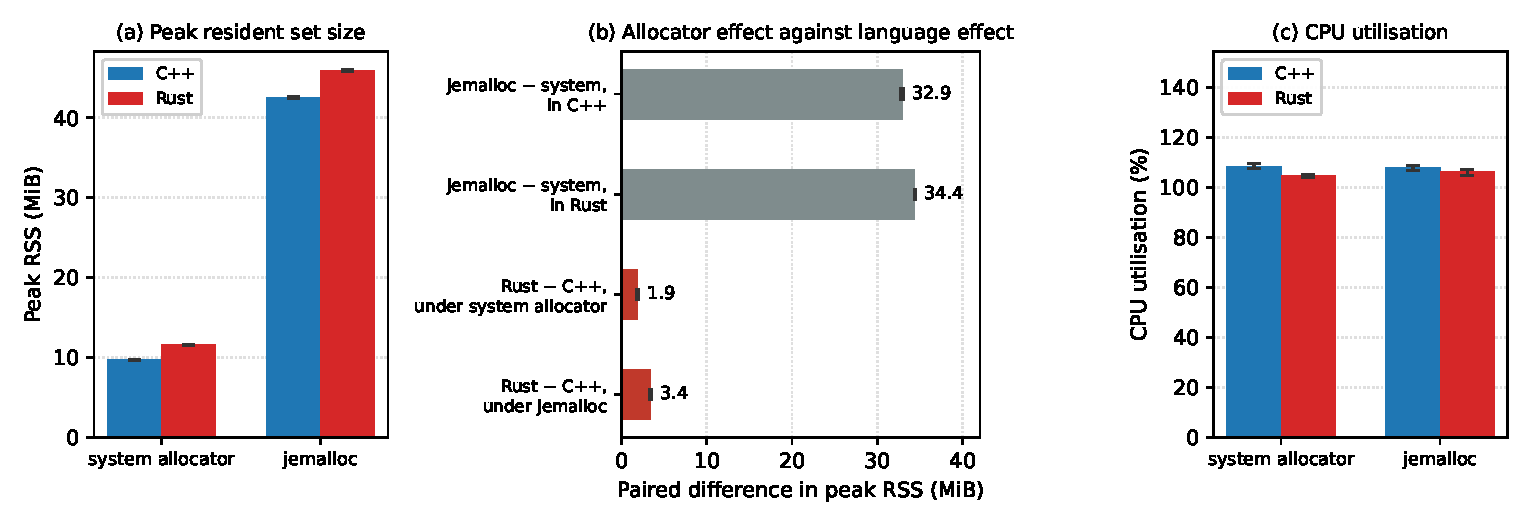
\includegraphics[width=\linewidth]{figures/fig_resources.pdf}
\caption[Resource use, and the two effects inside peak RSS]{Resource use at a sustained offered load of $\ReprLoad$~kops/s, grouped by allocator so
that the two bars in a group differ only in language and the two groups differ only in allocator.
Medians over \NRepeats{} repeats with bootstrap $95\%$ intervals. \textbf{(a)} Peak resident set
size. \textbf{(b)} The two effects it contains, each as a paired difference over the same
repeats: linking \texttt{jemalloc} costs $\RssAllocDiffLo$--$\RssAllocDiffHi$~MiB, while the Rust
build costs $\RssLangDiffLo$--$\RssLangDiffHi$~MiB more than the C++ one. Both are real, and on a
shared axis the allocator effect is an order of magnitude the larger. \textbf{(c)} CPU
utilisation, summed across threads, where the difference runs the other way and is
small.\label{fig:resources}}
\end{figure}

\subsection{Safety via fault injection (RQ2)}\label{sec:safetyresults}
Instead of claiming that Rust has no bugs, the catalogue of ten defects set out in
Table~\ref{tab:defectmap} is deliberately injected, each as a small self-contained program
flavoured with the subsystem's domain so that it maps onto a plausible bug in the service. Its
division into two groups is what the method of Section~\ref{sec:methodfaults} turns on: five
classes from inside the region Rust claims to govern, and five chosen precisely because safe
Rust is expected \emph{not} to prevent them. Without the second group the outcome would be
decided by the choice of test cases, confirming the expected result but never able to disturb
it. With it, the study measures a boundary rather than demonstrating a claim. The fault runner
holds the expectation recorded for each case in advance and reports a violation in either
direction, so a case that unexpectedly compiled, or unexpectedly failed to, would surface
instead of being absorbed into the conclusion.

\paragraph{Procedure.}
For each C++ defect the study builds and runs the program under AddressSanitizer (ASan),
ThreadSanitizer (TSan) and UndefinedBehaviorSanitizer (UBSan), and records which tool, if any,
detects it. The third is not a refinement of the other two but a separate axis: signed overflow
is invisible to both ASan and TSan, so without its own column the integer-overflow class would
be recorded as undetected in C++ when in fact it is caught. No static analyser is
run, for the reason set out in Section~\ref{sec:methodfaults}: its output is neither a
compile-time rejection nor an observation of an execution, so it does not belong to any of the
three outcomes the taxonomy records. The C++ columns of Table~\ref{tab:taxonomy} therefore
report the tooling this study ran rather than a ceiling on what C++ tooling could achieve. The
analogous construct is written in safe Rust and compiled. Where it compiles, it is then run
under a bounded timeout and its observable behaviour recorded, since ``it compiles'' alone would
not establish whether the defect survives into the running program. The catalogue, the runner,
and the raw tool logs are published with the thesis.

\paragraph{Results.}
The outcomes are shown in Table~\ref{tab:taxonomy}, measured with \texttt{g++~13.3}
(\texttt{-std=c++23}, \texttt{-O0} so the optimizer cannot elide an injected defect) and
\texttt{rustc~1.97} (edition~2021). That C++ toolchain is the local development machine's
and not the measurement host's \texttt{g++~15.1.1}, and the catalogue was run there
deliberately. Whether a program compiles, and what a sanitiser reports when it runs, are
properties of the toolchain rather than of the machine hosting it, which is the concrete
content of calling this result environment-insensitive in
Section~\ref{sec:testbed}. Within its scope the result is unambiguous. Every one of
the five memory-safety and data-race defects is a compile error in safe Rust, so none can be
written at all. In C++ each is valid code whose defect manifests only at runtime, and
only if a test actually exercises the buggy path. The memory-safety defects are caught by ASan;
the concurrency defects are caught only by TSan and are invisible to ASan; the overflow in the
boundary group is caught only by UBSan and is invisible to both. No single C++ sanitiser covers
the catalogue, and the three between them still leave four of the ten classes untouched.
Runtime detection further requires building a
dedicated instrumented binary and paying the sanitiser's time and memory overhead, whereas the
Rust errors are reported on every ordinary build regardless of test coverage. The parenthesised
codes are the \texttt{rustc} diagnostics that fire (for example \texttt{E0499}, conflicting
mutable borrows; \texttt{E0502}, a mutable borrow while a shared borrow is live; \texttt{E0382},
use of a moved value; \texttt{E0373}, a closure outliving borrowed data as it escapes to another
thread).

All five boundary cases behave as predicted and delimit the claim. Every one compiles in safe
Rust and every one misbehaves. The deadlock case hangs in both languages and had to be killed
by the harness timeout. The lost-update case terminates in both languages with a silently wrong
answer: against an expected total of $40\,000$ increments the safe-Rust program recorded
$35\,030$, losing $4\,970$, and the C++ program under ThreadSanitizer recorded $25\,448$,
losing $14\,552$. The reference cycle leaks in both, the release-build overflow produces a
wrong TEID in both, and a failure inside one shard worker takes down more than that shard in
both.

Two of the five are cases where the C++ tooling is \emph{ahead}, which is the outcome the
two-sided catalogue was built to be able to produce. LeakSanitizer, which ships inside ASan,
reports the C++ reference cycle as an unreachable allocation at exit. The safe-Rust cycle leaks
in silence, because leaking is safe in Rust by explicit design and nothing in the default
toolchain looks for it. That this is a property of the language rather than an artefact of the
injected example is visible in the work being done to change it: proposals to add garbage
collection to Rust are motivated precisely by shared-ownership structures that reference counting
expresses ``awkwardly, inefficiently, or both''~\cite{hughes2025gcrust}. UBSan reports the C++ overflow, because signed overflow is undefined.
The Rust overflow is \emph{defined} to wrap at \texttt{opt-level~=~2}, which leaves
\texttt{overflow-checks} off, so the program has a meaning and the meaning is wrong. That
second contrast is worth stating carefully, because it does not reduce to which language is
safer: defined-but-wrong is easier to debug than undefined-and-wrong and no less incorrect, and
neither is what ``memory safe'' is usually taken to promise.

The deadlock result needs a qualification the earlier reading of it did not have.
ThreadSanitizer does flag the inversion in C++, but only on a minority of runs: four of twelve
repeats here, six of twenty in a longer trial, while the program deadlocks on every one. The
mechanism is specific and it generalises beyond this catalogue. TSan builds its lock-order
graph from acquisitions that \emph{succeed}, so the cycle closes only when some thread completes
an inversion without blocking. A run in which the first inversion blocks produces one edge and
never the second, and the detector stays silent at exactly the moment the bug manifests. A
positive control that inverts the same two locks without ever blocking is reported every time,
which is what establishes that the detector was live rather than misconfigured. The honest
statement for this class is therefore that the tool catches the inversion the program survives
and is unreliable on the one that deadlocks, which is a materially different proposition for a
continuous-integration pipeline than a clean catch.

The distinction all of this exposes is precise, and it is the distinction the phrase ``thread
safety'' routinely blurs. Rust's concurrency guarantee is the absence of \emph{data races},
meaning unsynchronised concurrent access to the same location. It is not a guarantee about
\emph{lock-acquisition order}, nor about the \emph{atomicity of a composed operation}, nor
about leaks, wrapping arithmetic, or fault containment. The lost update remains the quietest
case, because no sanitiser reports it: with every access properly locked there is no race for a
race detector to find.

\paragraph{Where the boundary classes are caught, and at what cost.}
RQ2 asks not only which defects are prevented but at what stage the rest are detected, and for
the boundary group the sanitiser columns leave that half largely blank. Two Rust model
checkers answer it. Loom, which enumerates thread interleavings exhaustively under the C11
model, and Shuttle, which samples them with probabilistic concurrency testing, both report both
of the original boundary defects: Loom reports the deadlock as a closed cycle and fails the
lost-update assertion, and Shuttle does the same. Each is paired with a control in which the
defect is fixed (consistent lock order, and the read-modify-write held in one critical
section), and both controls come out clean, so the reports are attributable to the defects
rather than to the tools.

The cost is the part worth recording. Neither defect program runs under either checker as
written. Each had to be re-imported against the checker's own synchronisation and thread types,
because a tool that does not intercept the primitive cannot schedule it, and each had to be
shrunk to model size: the lost-update model drops from twenty thousand iterations per thread to
one, and the deadlock model loses the sleep that widens its window on real hardware. So the
answer for the Rust half of the boundary is \emph{detected at test time, after a rewrite},
against a C++ half where the sanitiser takes the program unchanged and, for these two classes,
finds one unreliably and the other not at all. The two halves point in opposite directions, and
neither language's story here is the simple one. The consequence for practice is developed in
Chapter~\ref{chapter:discussion}.

\paragraph{A defect that was not injected.}
Every outcome above comes from a defect written on purpose, which is the standing weakness of
the method: whoever assembles a catalogue already knows what safe Rust prevents. One case in
this study does not carry that weakness. A design review of the specification found that its
concurrency section prohibited submitting an operation outside the service's running window
(before \texttt{start()}, or after \texttt{shutdown()}), while neither implementation checked
for it. The prohibition was addressed to the caller with no mechanism behind it, and in that gap
the two languages did not fail alike. The C++ submit path indexes the shard vector that
\texttt{shutdown()} has cleared, which AddressSanitizer reports as a heap-use-after-free. Called
before \texttt{start()} it is a segmentation fault on the zero page. In Rust both calls were
already a panic, from the ordinary bounds check on the same indexing operation, without anyone
having designed for it.

What makes the case evidentially different is its provenance rather than its severity. It sat in
code written to be correct, in the arm whose safety claim rests on ThreadSanitizer, reachable
through the public API by calling documented operations in a documented order. It also survived
every check this study runs (six C++ test binaries, twenty-five Rust tests, $223$
hand-written and $9\,006$ generated conformance operations, and three sanitiser configurations
reported clean), for a single reason: none of them ever called an operation outside the running
window. ASan finds this defect only once a test drives it, which is exactly the property the cost
argument above attributes to runtime detection, observed here on the study's own artefact instead
of on a planted one.

The direction in which it must \emph{not} be over-read is the flattering one. Rust did not
prevent this at compile time, and nothing in the borrow checker knows that a service must be
started before it is used. What converted undefined behaviour into a diagnosable failure was a
slice bounds check, which is a runtime guarantee and therefore the same kind of assurance the
C++ sanitiser offers rather than the compile-time kind Table~\ref{tab:taxonomy} records. The
honest claim is that checking by default turned a specification gap into a panic, not that a
type system caught a lifecycle error. What is left is still the distinction this chapter keeps
returning to: a panic that names its cause on every build, against a heap-use-after-free that
needs an instrumented binary and a test that thinks to look. Both implementations now reject the
call explicitly, in both directions, and both suites cover it.

\begin{table}
\centering
\small
\caption[Defect-class taxonomy: measured outcomes]{Defect-class taxonomy: measured outcomes for the injected catalogue. C++ under
\texttt{g++~13.3} with ASan/TSan/UBSan. Rust under \texttt{rustc~1.97}, edition~2021. ``Compile
error'' means the safe-Rust program does not build, so the defect cannot be written. The lower
block is the boundary group: defect classes chosen because safe Rust is \emph{not} expected to
prevent them, and does not. Two of those five are the ones on which the C++ tooling is
ahead.\label{tab:taxonomy}}
\footnotesize
\setlength{\tabcolsep}{4pt}
\begin{tabular}{@{}l l l l l@{}}
\hline\hline
Defect class & ASan & TSan & UBSan & Safe-Rust outcome \\
\hline
\multicolumn{5}{@{}l}{\emph{Within the guarantee}} \\
Use-after-free            & detected     & detected     & not detected & compile error (E0499) \\
Double-free               & detected     & not detected & not detected & compile error (E0382) \\
Iterator invalidation     & detected     & detected     & not detected & compile error (E0502) \\
Data race                 & not detected & detected     & not detected & compile error (E0373$^{\dagger}$) \\
Unguarded shared mutation & not detected & detected     & not detected & compile error (E0502$^{\dagger}$) \\
\hline
\multicolumn{5}{@{}l}{\emph{Boundary of the guarantee}} \\
Lock-order deadlock$^{\ddagger}$ & not detected & intermittent$^{\S}$ & not detected & compiles, deadlocks \\
Lost update               & not detected & not detected & not detected & compiles, wrong result \\
Reference-cycle leak      & detected     & not detected & not detected & compiles, leaks \\
Integer overflow (release) & not detected & not detected & detected     & compiles, wrong result \\
Worker-failure blast radius & not detected & not detected & not detected & compiles, shard outage \\
\hline
\end{tabular}

\vspace{0.4em}
{\footnotesize\raggedright
$^{\dagger}$ Several diagnostics fire for these cases. The first is shown (the data race also
raises \texttt{E0382} and \texttt{E0502}, the unguarded mutation \texttt{E0524} and
\texttt{E0597}). \quad
$^{\ddagger}$ Neither ASan nor UBSan issues a report, because nothing is corrupted and nothing
is undefined: the instrumented binary simply deadlocks and is killed by the harness
timeout. \quad
$^{\S}$ ThreadSanitizer reports the lock-order inversion on a minority of runs, measured at
$4$ of $12$ repeats here and $6$ of $20$ in a longer trial, while the program deadlocks on
every one. The detector builds its lock-order graph from acquisitions that \emph{succeed}, so a
run whose first inversion blocks never completes the second edge of the cycle.\par}
\end{table}

Read as a whole the table makes two things visible at once: above the boundary rule the entire
Rust column is a compile-time rejection while the C++ columns are a patchwork of runtime
detections and outright misses, and below it the Rust column joins them, and on two rows
falls behind. Figure~\ref{fig:taxonomy} draws the same ten outcomes as a matrix, where that
change of character at the rule is the shape of the picture rather than something to be read off
row by row. The outcomes are generated from the runner's machine-readable log
(\texttt{faults/results/taxonomy.csv}), and the model-checking outcomes from
\texttt{faults/results/model\_checking.csv}. Table and figure come from the same log, so neither
can drift from the other.

\begin{figure}
\centering
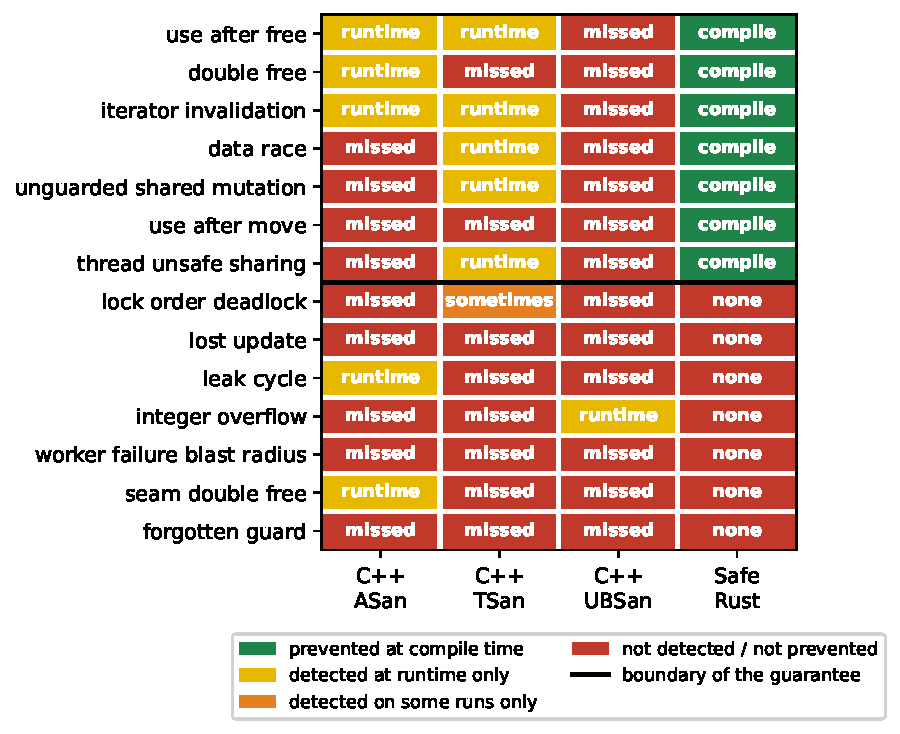
\includegraphics[width=0.92\linewidth]{figures/fig_taxonomy.pdf}
\caption[Where the guarantee stops: the outcome matrix]{The outcomes of Table~\ref{tab:taxonomy} drawn as a matrix, generated from the same
\texttt{faults/results/taxonomy.csv}. Above the rule the Rust column is a single colour: every
defect is a compile error, so none can be written. The C++ columns there are a patchwork instead,
and no one sanitiser covers the five. Below the rule the Rust column joins them, and on the
reference-cycle leak and the release-build overflow the C++ tooling is ahead. The lock-order
deadlock is the one cell where a tool reports intermittently: ThreadSanitizer flags the inversion
on a minority of runs while the program deadlocks on every one.\label{fig:taxonomy}}
\end{figure}

\subsection{Migration (RQ4)}\label{sec:migrationresults}
Incremental adoption is assessed with a working prototype that models the realistic
direction of migration: an existing C++ host keeps a Rust component behind a C ABI. The Rust
service is exposed through a thin \texttt{extern "C"} seam in a \emph{separate} crate that
depends on the unmodified core library, so adopting the component requires no changes to the
component itself. The C++ host sees only an opaque handle and a set of plain-C entry points
(a hand-written header, no generated bindings), and drives the full UE lifecycle across the
boundary. The error model is transported faithfully (for example, a duplicate connection
setup returns \texttt{InvalidState} through the seam). Figure~\ref{fig:ffiseam} shows the
resulting structure and where the \texttt{unsafe} sits.

\begin{figure}
\centering
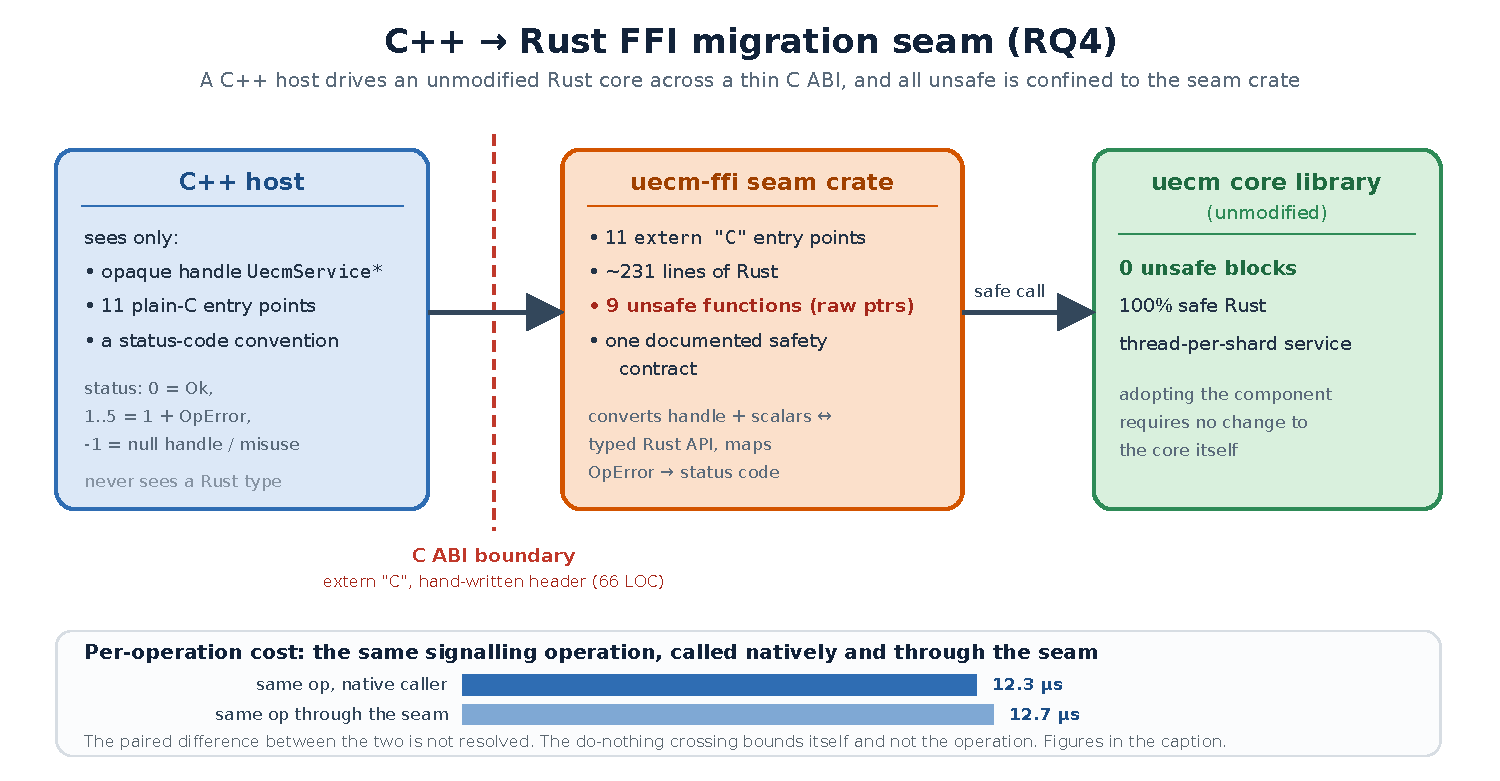
\includegraphics[width=\linewidth]{diagrams/pdf/07_ffi_seam.pdf}
\caption[The C++-to-Rust FFI migration seam]{The C++-to-Rust FFI migration seam. The C++ host sees only an opaque handle, $\FfiEntryPoints$
plain-C entry points, and a status-code convention. A thin \texttt{extern "C"} seam crate
concentrates all of the raw-pointer \texttt{unsafe} ($\FfiUnsafeFns$ functions) and calls the unmodified Rust
core, which remains free of \texttt{unsafe}. The do-nothing crossing costs $\FfiCrossing$~ns
against a $\FfiOpSeam$~\textmu s operation. Measured against the same signalling operation called
natively, the seam's cost per operation is bounded at $\FfiOpBoundPct\%$.\label{fig:ffiseam}}
\end{figure}

The prototype yields concrete interop-cost figures, summarised in Table~\ref{tab:ffi}. The
seam is small, $\FfiEntryPoints$ C-ABI entry points in $\FfiSeamLines$ lines of Rust plus a
$\FfiHeaderLines$-line C
header, with no third-party FFI dependency. The safety boundary is clean: the core library
remains free of \texttt{unsafe}, and the raw-pointer handling the C ABI requires is confined
to the seam crate (its $\FfiUnsafeFns$ \texttt{unsafe} functions) under a single documented safety
contract, so the C++ side never sees a Rust type.

The per-call cost is measured twice, because the two measurements answer different questions
and only the second answers RQ4's. The first is the intrinsic crossing: a do-nothing
\texttt{extern "C"} call costs $\FfiCrossing$~ns, an ordinary indirect call, and negligible
next to the microsecond-scale round-trip of a signalling operation. That bounds the
crossing but says nothing about what the seam does to a real operation, because an empty call
and a full round-trip are not the same experiment: the round-trip is dominated by a
cross-thread handoff, and an argument that the handoff ``would be paid identically anyway'' is
reasoning standing in for a measurement.

The measurement is therefore made directly. The same signalling operation, on the same service
configuration and in the same loop, is invoked natively from Rust and then from C++ through the
seam, interleaved over \FfiOpRepeats{} repeats so the pair is matched. The paired difference is
$\FfiOpDelta$~ns per operation with a bootstrap interval of $[\FfiOpDeltaLo, \FfiOpDeltaHi]$~ns
and an exact paired $p$ of $\FfiOpP$: no cost is detected, and more usefully, the interval
bounds any cost the measurement could have missed at $\FfiOpBoundPct\%$ of the operation. The
interleaving is not optional here. A single pass of each, run while preparing this section,
made the seam appear \emph{faster} than calling natively by a third, because the run-to-run
spread of the handoff on a shared host is far wider than anything a C ABI could contribute.
Figure~\ref{fig:fficost} shows the repeats that produced those numbers, and the left panel is
that spread: the pairs cross, and the range they cover is an order of magnitude wider than the
difference under test.

\begin{figure}
\centering
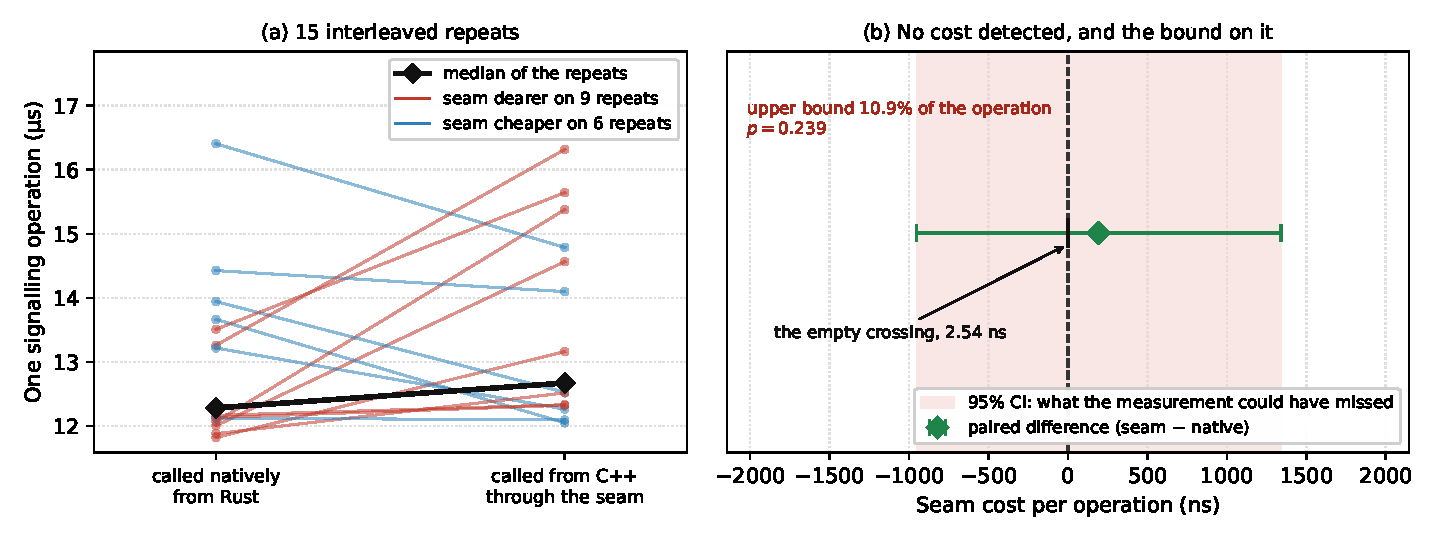
\includegraphics[width=\linewidth]{figures/fig_ffi_cost.pdf}
\caption[The seam's cost on one operation, against its own uncertainty]{The interoperability cost measured on a real operation rather than inferred from an empty
call. \textbf{(a)} The same signalling operation invoked natively from Rust and from C++ through
the seam, one line per interleaved repeat, with the medians in black. \textbf{(b)} The pairs
reduced to their difference: $\FfiOpDelta$~ns per operation with a bootstrap $95\%$ interval of
$[\FfiOpDeltaLo, \FfiOpDeltaHi]$~ns and an exact paired $p$ of $\FfiOpP$. No cost is detected, and
the upper end of that interval is what bounds the cost the measurement could have missed at
$\FfiOpBoundPct\%$ of the operation. The empty \texttt{extern "C"} crossing, $\FfiCrossing$~ns, is
marked for scale rather than as the answer: it is indistinguishable from zero on the axis the
operation is measured on.\label{fig:fficost}}
\end{figure}

The main engineering effort is therefore in \emph{designing} a C-compatible API
surface, an opaque handle, scalar-typed operations, and a status convention, rather than in
any runtime overhead. The reverse direction (Rust calling into C++) is symmetric but requires
a C-ABI wrapper on the C++ side and re-introduces \texttt{unsafe} at the Rust caller. The
prototype and its measurements are published with the thesis, and inform the migration
guidelines of Chapter~\ref{chapter:discussion}.

\begin{table}
\centering
\caption[FFI migration prototype: seam size, safety, and cost]{FFI migration prototype: seam size, safety boundary, and per-call interop cost
(C++ host calling the Rust component across a C ABI, \texttt{-O2}). The core library is
unmodified and \texttt{unsafe}-free. All interop is confined to the seam crate. The last
three rows are the direct comparison: one signalling operation on the same service
configuration and the same loop, invoked natively and then through the seam, so the
difference isolates what the boundary adds rather than what the operation
costs.\label{tab:ffi}}
\begin{tabular}{l r}
\hline\hline
Metric & Value \\
\hline
C-ABI entry points & 12 \\
Seam size (Rust \texttt{lib.rs}) & 231 LOC \\
Hand-written C header & 66 LOC \\
\texttt{unsafe} in core library & 0 \\
\texttt{unsafe} in FFI seam & 12 \\
Raw FFI crossing & 2.54 ns/call \\
Signaling op, native caller & 12.3 \textmu s/call \\
Signaling op, through the seam & 12.7 \textmu s/call \\
Seam cost per operation (paired) & $+192$ ns $[-954, +1341]$ \\
\quad as a fraction of the operation & $+10.91\%$ at the upper bound
\\
\hline
\end{tabular}
\end{table}

\chapter{Discussion\label{chapter:discussion}}

\section{Summary of findings}
Table~\ref{tab:findings} collects the headline finding for each research question together with the
strength of the current evidence. The safety and migration results (RQ2, RQ4) do not depend on the
measurement environment at all. The performance and resource results do, and the honest division
is no longer between chapters but within RQ1: the saturation knee, the overload comparison, and the
resource comparisons are resolved on the host of Section~\ref{sec:testbed} and replicate across the
allocator control, while the far tail below saturation remains unresolved for reasons that belong
to the machine rather than to the analysis.

\begin{table}
\centering
\caption[Summary of findings per research question]{Summary of findings per research question and the current strength of evidence.
\label{tab:findings}}
\renewcommand{\arraystretch}{1.25}
\begin{tabular}{@{}p{0.06\linewidth} p{0.62\linewidth} p{0.22\linewidth}@{}}
\hline\hline
RQ & Headline finding & Evidence status \\
\hline
RQ1 & The answer divides at saturation. Below it the variants agree to $\PFiftyRange\,\mu$s
($\PFiftySpread\%$) at the median and no tail ordering is resolvable. The end-to-end number is
only $\BudgetCoreShareMax\%$ operation, so it cannot bound a language effect in any case, while
the operation measured apart is $\BudgetCoreRatio\times$ faster in \BudgetCoreFaster. Past
saturation they diverge decisively: \OverloadSustainedFaster{} sustains
$\OverloadThrRatio\times$ the throughput of \OverloadSustainedSlower{} at
$\OverloadLoad$~kops/s, in \OverloadThrAgree{} repeats under both allocators. & Overload and
operation: resolved. Far tail: unresolved on this host. Mechanism: tested. Primitives alone
insufficient \\
RQ2 & All five injected memory-safety and data-race classes are prevented at compile time in
safe Rust, where in C++ each compiles and is caught, if at all, only at runtime and by no single
sanitiser. The guarantee stops there: the five boundary classes compile in both languages, and
on the leak and the release-build overflow the C++ tooling reports what Rust's does not. &
Final \\
RQ3 & A memory penalty that reproduces: $\RssLangDiffLo$--$\RssLangDiffHi$~MiB more peak RSS in
the Rust build under \emph{both} allocators, an order of magnitude less than the allocator's own
$\RssAllocDiffLo$--$\RssAllocDiffHi$~MiB. CPU inverts across the regimes: Rust draws up to
$\CpuDiffAbsMax$ percentage points less below saturation and $\OverloadCpuPerOpRatio\times$ more
per completed operation above it. & Memory: resolved, unexplained. CPU: resolved in both
regimes, opposite signs \\
RQ4 & The seam is small and keeps the core \texttt{unsafe}-free at compile time. Measured against
the same operation called natively, no cost is detected and any tax is bounded at
$\FfiOpBoundPct\%$ of an operation. The real cost is API design. The core remains exposed at run
time to memory errors in the C++ host it shares an address space with. & Final \\
\hline
\end{tabular}
\end{table}

\section{Discussion on the research questions}\label{sec:rqdiscussion}
\paragraph{RQ1 (predictability).} RQ1 has two halves, below saturation and beyond it, and the
campaign answers them differently enough that reporting either alone would misrepresent the
result.

Below saturation the languages are equivalent in central behaviour, and by a margin no deployment
would notice: the small paired difference at the median that does clear the correction is a
fraction of an $80\,\mu$s operation. The far tail in this regime is a different matter, and one a
deployment would also care about. There the result is a null this host cannot turn into an
ordering, so the equivalence claimed here does not extend to it. That is consistent with the wider evidence that
Rust's safety checks are largely absorbed by modern out-of-order
CPUs~\cite{balasubramanian2017rust,emmerich2019drivers}. It is also a weaker statement than it
appears, for the reason Section~\ref{sec:budget} gives: the operation the
languages execute is $\BudgetCoreShareMax\%$ of what the sweep measures, so an end-to-end null in
a design dominated by a cross-thread wakeup is a statement about the design rather than about the
languages. Measured apart, the operation differs by $\BudgetCoreRatio\times$.

Beyond saturation the answer changes in kind, and it is the one result in the study that answers
RQ1 on RQ1's own terms. The C++ build sustains $\OverloadThrRatio$ times the throughput of the
Rust one while drawing more CPU per completed operation, reproducibly and at the corrected floor
of the whole test family (Section~\ref{sec:overload}). So the practical form of RQ1's answer is
not that the language choice is irrelevant to predictability
but that it is irrelevant \emph{until the service stops coping}, at which point it decides how
much work still gets done. A comparison that stopped at nominal load, as most in this literature
do, would have concluded the opposite with the same apparatus.

That reframes the closest prior work instead of merely agreeing with it. Arvidsson and Kaller
measure this quantity for 5G control-plane procedures and find Rust's 99th percentile degrading
faster beyond a threshold request rate, which they trace to stackless
\texttt{async}/\texttt{await} permitting a context switch immediately before an I/O operation
begins~\cite{arvidsson2025async}. Section~\ref{sec:relatedwork} accepts that attribution, and
this study was built to exclude the confound behind it: one worker per shard over a bounded
blocking queue, no asynchronous runtime on either side. Section~\ref{sec:rqs}
committed in advance to what each outcome would mean, and the second branch is the one that
fired. A degradation past a threshold rate appeared with the concurrency model held fixed, so the
asynchronous runtime cannot be the only place such an effect originates. The prediction also
named where to look first if that happened, bounds and overflow
checking~\cite{zhang2022runtime,harris2023morello}. That part of it was wrong. The effect
appears only once the handoff path is contended, which points at the two standard libraries'
blocking primitives recorded in Table~\ref{tab:idioms}. Section~\ref{sec:contention} then tests
whether those primitives alone explain the gap and finds they do not reproduce the full-service
ordering at significance, which narrows the cause to additional work on the C++ handoff path
rather than to the safety model. Recording that the prediction resolved against its own first
hypothesis, and that the follow-up microbenchmark refined the attribution instead of confirming it,
is more useful to the next study than quietly substituting the explanation that survived.

\paragraph{RQ2 (safety).} The result does not depend on the environment, and what makes it
interesting is not the half that confirms the expectation but the half that bounds it. Within
its scope the guarantee is absolute in one specific sense, and the difference from C++ is one of
kind rather than of degree: a compiler that refuses to build a program rules the defect out of
every execution, where a sanitiser rules it out only of the executions an instrumented test
happens to take. What is absolute is the execution coverage, not the breadth of the catalogue.
The scope itself remains the ten programs written for it.
That aligns with the CVE evidence that Rust memory-safety bugs invariably involve
\texttt{unsafe}~\cite{xu2021rustcve} and with the caution that unsafety can still propagate
through dependencies~\cite{evans2020rust}, which is why keeping the core \texttt{unsafe}-free
matters.

The one case that reaches past the ten programs is the lifecycle defect of
Section~\ref{sec:safetyresults}. It was found in the implementation rather than written for
the catalogue, and it revises the picture in two directions at once. It strengthens the cost
argument. A real defect in code written to be correct survived the entire verification
apparatus of this study (tests, parity vectors, and three sanitisers) purely because
nothing exercised the path. Runtime detection conditional on test coverage is a weaker
proposition in practice than it looks in a table where every row is driven deliberately. It also
narrows what may be credited to Rust, because the language's contribution there was a bounds
check rather than a proof. Safe Rust turned undefined behaviour into a deterministic panic, which
is a different and lesser claim than preventing the error. The honest generalisation is that
the guarantee worth budgeting for is \emph{checked by default} rather than \emph{ruled out at
compile time}. The defect's root cause is worth naming too, because it is a risk of the method
and not of either language: a specification that states a prohibition without assigning a
mechanism leaves each implementation to fail in its own idiom. The two idioms here are a
panic and a use-after-free.

Where the guarantee stops matters just as much to a vendor deciding what Rust buys, and the two
boundary classes are instructive for different reasons. The lock-order deadlock shows that Rust
reasons about \emph{aliasing}, not about \emph{acquisition order}. A \texttt{Mutex} guard is an
ordinary value whose lifetime the borrow checker tracks perfectly, and tracking it perfectly
says nothing about whether two threads take their locks in compatible orders. That this is a
boundary of the language rather than an artefact of the injected example is confirmed by the
tooling built around it, since static deadlock detection for Rust is an active research problem
in its own right~\cite{zhang2026deadlock} and model checkers for Rust kernel code are motivated
explicitly by the observation that ownership and borrowing leave data races, deadlocks, and
livelocks reachable~\cite{tang2025converos}. The lost update is sharper still. It escapes
ThreadSanitizer for precisely the reason it escapes the borrow checker, which
Section~\ref{sec:safetyresults} sets out: with every access correctly synchronised there is no
unsynchronised access to find. The distinction it exposes, between a data race and a race
condition, is the one the phrase ``thread safety'' routinely conflates, and Rust removes only
the first.

The practical consequence is that adopting Rust retires one category of concurrency defect
completely while leaving another untouched. The category left untouched is the one that fails
silently, corrupting a counter or a state decision instead of crashing. A migration plan that
treats ``memory-safe'' as ``concurrency-safe'' would therefore mis-budget its review and testing
effort. That is why this boundary is reported as a first-class result rather than a caveat.
Figure~\ref{fig:boundary} states the whole result in one picture, with the two halves of the
guarantee on either side of the line and the mechanism that does the enforcing, or the absence
of one, named in each panel.

\begin{figure}
\centering
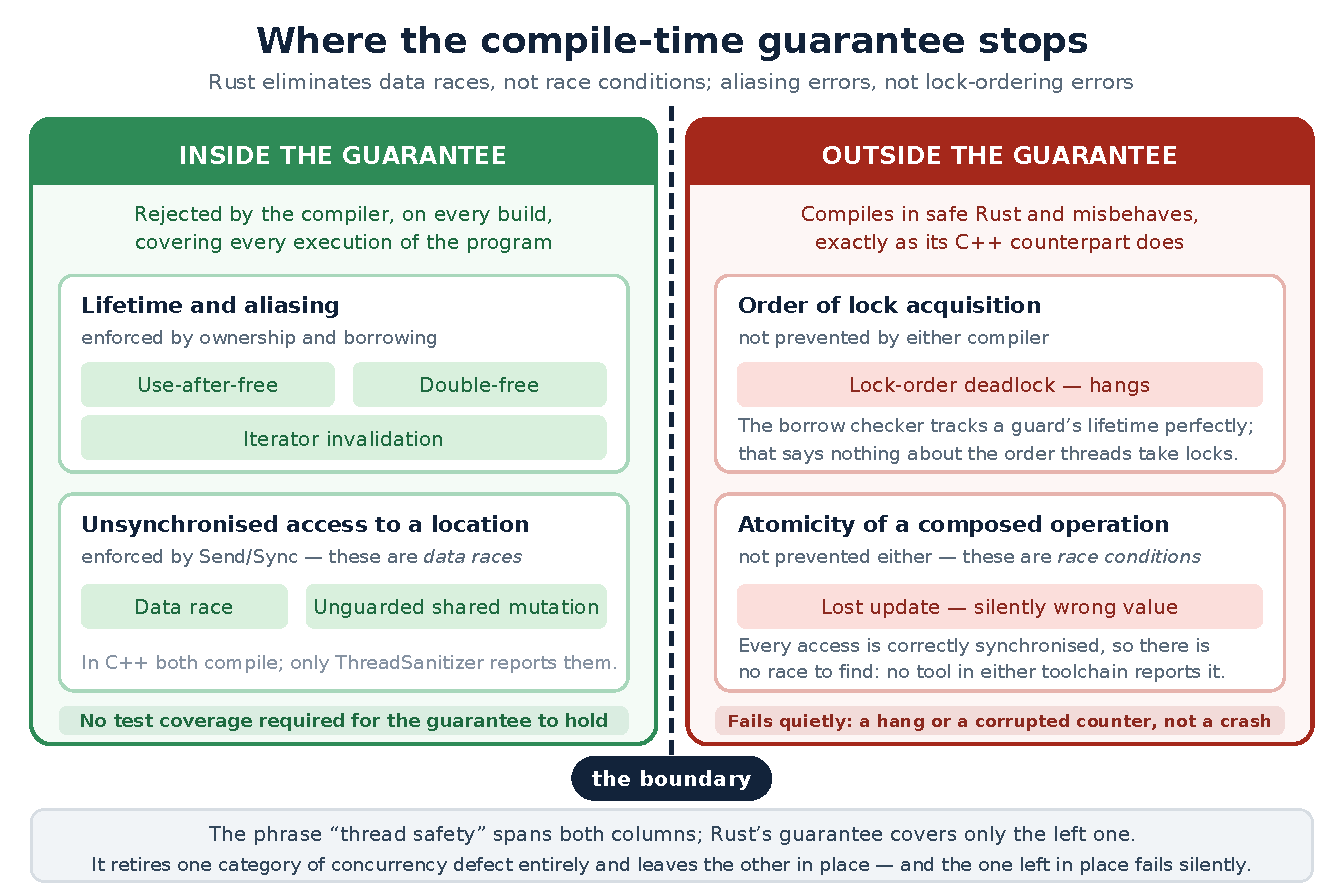
\includegraphics[width=\linewidth]{diagrams/pdf/17_guarantee_boundary.pdf}
\caption[Where Rust's compile-time guarantee stops]{Where the compile-time guarantee stops. On the left are the classes safe Rust rejects
outright, grouped by the \emph{mechanism} that rejects them rather than by defect
family: ownership and borrowing for lifetime and aliasing errors,
which is why iterator invalidation sits with them, and the \texttt{Send}/\texttt{Sync}
discipline for unsynchronised access to a location. On the right are the classes the
catalogue included to find the edge, which neither compiler prevents. The diagram shows the two
concurrency cases, and the leak, the release-build overflow and the worker-failure case added
later sit alongside them. The phrase ``thread safety'' spans both sides of the line. The
guarantee covers only the left.\label{fig:boundary}}
\end{figure}

\paragraph{RQ3 (overhead).} The answer splits by resource, and the splits do not all point the
same way. On memory there is a penalty: the Rust build carries a few MiB more peak resident set
than the C++ build, and keeps that sign under both allocators. Two things make it credible beyond
the $p$-value. Peak RSS is a run-level maximum rather than a
tail statistic, so it is insensitive to the scheduling jitter that destroys the p99. And the
effect is an order of magnitude smaller than the allocator's own, which is the useful way to size
it: a team choosing between these two languages moves less memory than a team choosing between
these two allocators.

On CPU the answer depends on the load, and that dependence is the finding rather than a
complication. Below saturation Rust draws marginally \emph{less}, consistently under both
allocators. Past saturation the sign inverts and the magnitude grows
(Section~\ref{sec:overload}). A single number for ``the CPU cost of
Rust's safety model'' would therefore be an average over two regimes that behave oppositely, and
neither figure is the safety model in any case. On throughput the same split applies for the same
reason: below saturation there is nothing to measure, because achieved throughput tracks offered
load by construction, and above it there is the largest effect in the study.

Three things bound what the memory result licenses. It is small in absolute terms and, more
importantly, it is fixed rather than per-context, so its share of a deployment's footprint
falls as the deployment grows. The measured layout difference between the two
\texttt{UeContext} types contributes almost none of it. It is also unexplained. Attributing it
between allocator arena reservation, per-thread caches, and static footprint needs allocation
profiles and hardware counters this study did not collect, which is the single clearest gap in
the RQ3 instrumentation. And it should not be generalised into a claim about Rust's safety
model, since nothing here isolates bounds checking or ownership-driven copying as the cause.
The mechanisms that the literature has localised~\cite{zhang2022runtime,harris2023morello}
are candidates to test, not conclusions to import. What can be said is narrower and still
useful to a vendor sizing a control-plane node: adopting Rust here costs a few megabytes of
fixed footprint per process, and buys a faster core operation
(Section~\ref{sec:budget}) that this workload's structure never converts into throughput below
saturation and, above it, converts into a deficit instead of a gain.

The sign of that result is worth defending, because one of the closest prior works in the domain
reports the opposite one, while two others agree with it. Agreement first, since it is quickly
stated: a second Ericsson-hosted study of RAN node management software found Rust's peak memory
usage generally higher than C's~\cite{olsson2023ranmgmt}, and a matched pair of user-space device
drivers outside telecom put the Rust version's footprint about 29\% above the C
version's~\cite{sundvisson2026drivers}. Neither separates the allocator from the language, which
is the distinction Section~\ref{sec:resources} rests on, so they corroborate the direction of the
effect and not its decomposition.

The disagreement is the more instructive case. Karlb\"ack and Or\"o measure peak resident set on a RAN workload and
find Rust the \emph{lowest} of the three languages and C++ the highest, with the gap widening
as concurrency rises, a pattern they call surprising and attribute tentatively to the initial
stack size of the green threads~\cite{karlback2021ran}. The two
findings are compatible once it is seen that they measure different quantities. Their C++ runs
on Boost.Fibers, which allocates a stack per fiber, so ten thousand concurrent sequences cost
ten thousand stacks. Their Rust runs on Tokio, where a task is a heap-allocated future of a few
hundred bytes. What their figures capture is therefore the per-context cost of the concurrency
runtime, which is precisely why it grows with the number of contexts. The design measured here
has no green threads on either side: a fixed thread-per-shard pool leaves no per-context
allocation to differ, and what remains is the fixed footprint reported above, constant in the
number of UEs and not proportional to it. Their disagreement with this result is thus
between two concurrency runtimes rather than between two languages, which is as direct a
demonstration as the literature offers of why this study holds the concurrency model fixed. It
also sharpens the caveat attached to the present number: it licenses nothing about Rust's
memory behaviour under a task-per-UE design, which is a different experiment.

\paragraph{RQ4 (migration).} The prototype shows that incremental adoption is technically
cheap: a C++ host can call an unmodified Rust core across a thin C-ABI seam whose cost on a
real operation is bounded at $\FfiOpBoundPct\%$, confining all \texttt{unsafe} to the seam.
That bound comes from the matched comparison of Section~\ref{sec:migrationresults}, not
from setting an empty crossing
against a full round-trip. The two are not the same experiment, and on this host a single
unpaired pass of each was enough to invert the apparent ordering. The dominant cost is
therefore human, not machine: designing a C-compatible surface and, per adoption
studies~\cite{fulton2021adopting,crichton2024learning}, climbing Rust's learning curve. This
reframes migration risk as an organisational rather than a performance concern, and the two
largest documented adoptions into existing C and C++ codebases report the same ordering of
costs~\cite{li2026rustlinux,fan2026android}.

One boundary on that result has to be drawn explicitly, because the natural reading overstates
it. ``All \texttt{unsafe} confined to the seam'' is a claim about what the compiler verifies,
and it is true as measured: the core crate contains no \texttt{unsafe}, and every raw-pointer
operation sits in $\FfiUnsafeFns$ reviewable functions. It is not a claim that the core is protected at run
time. Host and component share an address space, and a memory error on the C++ side can corrupt
Rust-owned data regardless of how the Rust side was checked, which is why the remedies proposed
in the literature isolate the two heaps with hardware support instead of relying on interface
discipline~\cite{rivera2021galeed,kirth2022pkrusafe}. The defect classes that arise at such
boundaries have been catalogued in their own right~\cite{li2022crosslang}. So what a migration
of this shape buys is narrower than ``the Rust part is safe'': it is that the migrated
component stops \emph{contributing} new memory-safety defects, while remaining exposed to those
of the host until the host is migrated too. That is still the right direction of travel, and it
is a reason to sequence a migration so that the components sharing the most mutable state cross
over together rather than one at a time.

\section{Revisiting the hypotheses}\label{sec:hypotheses}
Section~\ref{sec:rqs} committed to three hypotheses before any measurement was
taken. Stating their disposition explicitly, rather than letting the results speak for
themselves, is what distinguishes a test from a description.

\begin{description}
  \item[H1: supported below saturation, refuted above it.]
        The hypothesis had two parts: that the languages are performance-equivalent below
        saturation, and that any difference is confined to the far tail. The first is
        supported. The second is refuted, and not in the direction the wording anticipated,
        for the reasons Section~\ref{sec:rqdiscussion} gives. The far tail below saturation,
        which is what H1 actually named, remains unresolved on this host. The difference that
        did appear lies in overload. The hypothesis as written would have led the campaign to
        look in the wrong place, and the result was found only because the sweep was pushed
        past saturation on methodological grounds rather than in expectation of it.

        A second disposition is that the hypothesis is not well posed.
        ``Performance-equivalent'' was written as though it named one quantity, and
        Section~\ref{sec:budget} shows it names at least three: the delivered operation below
        saturation, where the languages are equivalent; the code the compilers emit, where they
        are not and the end-to-end measurement dilutes the difference by more than two orders of
        magnitude; and sustained work under overload, where they are not equivalent either and
        the difference runs the other way. All three are true, and a hypothesis that cannot
        distinguish them is one this study should have stated more carefully before measuring.
  \item[H2: supported in its precise form, refuted in its loose one.] The hypothesis was
        that safe Rust prevents at compile time ``the memory-safety and concurrency defect
        classes that C++ leaves to best-effort detection''. For the five injected classes of
        that kind it holds without exception. The fault-injection study still refutes
        the broader reading the wording invites: the five boundary classes are exactly the sort
        C++ leaves to best-effort detection, safe Rust does not prevent them either, and on the
        leak and the release-build overflow the C++ tooling is the one that reports. H2 is
        therefore accepted for memory safety and
        data-race freedom and rejected for concurrency correctness at large, and the latter is
        the reading practitioners tend to assume.
  \item[H3: supported, and tested the right way on the second attempt.] The hypothesis was
        that interoperability cost is negligible against the operations invoked. Measured
        directly (Section~\ref{sec:migrationresults}), no cost is detected and any per-operation
        tax is bounded at $\FfiOpBoundPct\%$. The bound, rather than the failure to detect a
        difference, is what supports the hypothesis. The first version of this measurement did
        not do that: it set an empty crossing against a full round-trip and inferred the
        answer, which is a comparison between two different experiments and would have given
        the right conclusion for the wrong reason. The accompanying claim, that the real cost
        is engineering effort, is supported structurally and not statistically: the seam is
        small and mechanical, but designing its C-compatible surface was the part of the
        prototype that required actual design decisions.
\end{description}

\section{Engineering guidelines for incremental adoption}
\label{sec:guidelines}
The results are meant to be usable, and a vendor weighing Rust for a control-plane component
needs more than a set of measurements. The following guidelines are the practical form of the
evidence above. Each is tied to the finding that supports it, and the boundaries of that
support are stated rather than glossed, because a guideline quoted without its limit is how the
RQ2 result becomes ``the migrated component is safe'' and the RQ4 result becomes ``migration is
cheap'', neither of which this study establishes. They are given in the order a first migration
would run them.

\paragraph{Choose the first component for its interface, not its size.}
Because the boundary's run-time cost is bounded at $\FfiOpBoundPct\%$ of an operation (RQ4), the
criterion for a first Rust component is not how small or how hot it is but how narrow and how
scalar its interface is. The seam here stayed at $\FfiEntryPoints$ entry points because the subsystem's API
was already lifecycle-oriented, typed, and free of shared mutable structures crossing the
boundary. A component whose interface passes rich C++ objects, templates, or callbacks will need
those designed out first, and that redesign, not the FFI, is the schedule risk.

\paragraph{Put the ABI in its own crate and keep the core \texttt{unsafe}-free.}
Concentrating every raw-pointer operation in a separate seam crate depending on an unmodified
core (Section~\ref{sec:migrationresults}) is worth adopting as a rule instead of treating as an
accident of this prototype: it keeps the dependency-propagation problem Evans et al.\
describe~\cite{evans2020rust} away from the safety-critical code, and makes the reviewable
surface of the migration a fixed, countable thing. Two qualifications belong with it. It bounds
what has to be \emph{reviewed}, not what can be \emph{corrupted}: while the host remains C++ the
two share a heap, so a team needing the stronger property must look at in-process
isolation~\cite{rivera2021galeed,kirth2022pkrusafe} and not at interface discipline alone.
And the generated part of a seam is not above suspicion, since binding generators have their own
defect history~\cite{cai2026interop}. Review it as code rather than trusting it as tooling
output.

\paragraph{Do not re-budget concurrency review effort on the strength of memory safety.}
This follows directly from the boundary cases. Adopting Rust removes use-after-free,
double-free, iterator invalidation, and data races from the defect budget entirely, and those
are the classes that dominate the security statistics~\cite{msrc2019memory,google2022android}.
It removes nothing from the deadlock and atomicity-violation budget. Lock-ordering discipline,
invariants about which locks may be held simultaneously, and review for
composed-but-not-atomic operations remain exactly as necessary as they were in C++, and they
should stay in the code-review checklist and the design-review agenda after migration.

\paragraph{Prefer a shared-nothing structure to a shared-and-locked one, in either language.}
The strongest concurrency result in this study is not attributable to either language: the
thread-per-shard design removes locks from the hot path altogether, which is why the boundary
defects had to be constructed as standalone programs rather than found in the implementations.
Where state can be partitioned by a natural key, as UE state can be partitioned by
\texttt{ue\_id}, partitioning it converts a class of concurrency defects into a structural
impossibility for both languages, and it does so without needing either compiler's help.

\paragraph{Budget for the learning curve, and measure it.}
The dominant cost identified here is human, matching what adoption studies
report~\cite{fulton2021adopting}. This thesis cannot quantify that cost, because it is a
single-author study, and the guideline is correspondingly modest: treat the first component as
a training investment with a deliberately generous schedule, and instrument it, recording
review time and defect density, so the second component can be planned on measured rather than
assumed effort.

\paragraph{Measure the component, not the round-trip, and do not generalise either.}
The performance findings carry a methodological warning that generalises further than the
numbers do. An end-to-end request/response measurement of a design like this one is
$\BudgetCoreShareMax\%$ language and the rest scheduler (Section~\ref{sec:budget}), so below
saturation it will return ``no difference'' between almost any two competent implementations,
and reading that as evidence about the languages is a mistake this study made before it measured
the components apart. A vendor running its own comparison should budget for both: the
end-to-end measurement, which says what a deployment will feel, and the component one, which
says what the language is doing.

\paragraph{Sweep past saturation, because that is where the languages stopped agreeing.}
This is the guideline the study would most like to have followed from the start rather than
arrived at. Every conclusion it drew about performance while the sweep stopped at nominal load
was a null, correct at that operating point and silent about the one where the two
implementations differ by $\OverloadThrRatio\times$ (Section~\ref{sec:overload}). The knee is
not a detail at the edge of the graph: for a control plane it is the region that decides whether
a signalling storm degrades service or ends it, and it is where a bounded, blocking design has
no graceful behaviour left. A comparison that stops while the system is still meeting its
offered load has measured the easy half of the question, and sweeping past the knee costs one
more afternoon of machine time.

Beyond both of these, the benchmarking framework rather than its current output is the reusable
artifact: the decision it should inform is ``measure this on your component, and measure it past
the point where your component stops coping'', not ``Rust is fast enough, proceed''.

\section{Related work}\label{sec:relatedwork}
Chapter~\ref{chapter:background} set out the ground this work stands on. What follows positions
the thesis against that literature rather than surveying it a second time, and then treats at
length the two studies it has to answer to.

Four strands bear on the comparison, and Chapter~\ref{chapter:background} sets out each of them.
What matters here is the property they share. Cross-language performance measurement puts
compiled systems languages close together on time and
energy~\cite{bugden2022rust,pereira2017energy} and finds Rust's safety cheap at run
time~\cite{balasubramanian2017rust,levy2017kernel}, including where timing is tightest: embedded
hypervisors~\cite{mo2023rustshyper}, production cloud infrastructure~\cite{agache2020firecracker},
packet processing within a few percent of a C
reference~\cite{emmerich2019drivers,xiao2024rpkt}. Where a cost does appear it has begun to be
localised, to bounds, overflow and division checks~\cite{zhang2022runtime}, to the bounds check
set against hardware-enforced capabilities~\cite{harris2023morello}, and to recurring
anti-patterns~\cite{cui2025perfbugs}. All of it is average-case. None of it reports behaviour past
a saturation point, which is the regime this thesis targets. The evidence for the safety claim is
settled in the same partial way: machine-checked foundations for the safe fragment and for the
aliasing discipline \texttt{unsafe} code must
respect~\cite{jung2018rustbelt,jung2021safe,jung2020stacked}, confirmation that \texttt{unsafe} is
used sparingly and that memory-safety CVEs invariably involve
it~\cite{qin2020rust,astrauskas2020unsafe,xu2021rustcve}, ecosystem-scale auditing that finds
defects at scale regardless~\cite{bae2021rudra,zheng2024security,qin2024safety}, the caution that
unsafety propagates through dependency chains~\cite{evans2020rust}, and the reports motivating the
shift against a long record of memory corruption resisting runtime
mitigation~\cite{msrc2019memory,google2022android,google2024securebydesign,cisa2023memorysafe,oncd2024building,szekeres2013sok}.

The third strand qualifies the adoption argument, and Section~\ref{sec:interop} states its central
limit: confining \texttt{unsafe} to a seam does not protect the Rust side, because foreign code in
the same address space can corrupt Rust-owned data
regardless~\cite{rivera2021galeed,kirth2022pkrusafe}, the seam has its own defect
classes~\cite{li2022crosslang}, and its tooling its own bugs~\cite{cai2026interop}. Lighter
crossing models exist for embedded use~\cite{schuermann2023encapsulated}. What that section does
not cover is reach. Aliasing patterns expressible in C but not in safe Rust bound translation in
principle~\cite{emre2023aliasing}, interoperation is the central open problem in embedded
Rust~\cite{sharma2024embedded}, \texttt{unsafe} concentrates at exactly these
boundaries~\cite{mccormack2026unsafe}, and the two largest documented adoptions into existing C
and C++ report the resulting friction empirically~\cite{li2026rustlinux,fan2026android}.
Automating the rewrite is an active line of work rather than a solved problem, current translators
still emitting code whose safety the compiler cannot validate~\cite{hong2025ctorust}, which is why
the migration cost measured here is the cost of a hand-written seam.

The fourth strand is the domain and the method: the tail-latency and microsecond-scale
literature~\cite{dean2013tail,barroso2017microseconds,li2014tales,huang2017predictability},
thread-per-core structuring moving the tail in its own right~\cite{enberg2019threadpercore}, O-RAN
disaggregation~\cite{polese2023oran}, control-plane latency as an active target in the core network
too~\cite{liu2023l25gc,park2025ctrlbench}, adoption evidence pointing at the learning curve rather
than run-time cost~\cite{fulton2021adopting,crichton2024learning,ardito2021verbosity}, and standard
guidance on repeat-based evaluation~\cite{georges2007rigorous} and fault
injection~\cite{natella2016fault}. Rust has mobile-network precedent in the
datapath~\cite{qazi2017pepc} and, on the control-plane side, an open-source gNB-CU with a separated
CU-CP and CU-UP over E1. That last one bears on the gap rather than on the method. It establishes
that the ASN.1 and SCTP protocol surface is no barrier in principle, but it is an existence proof
and not a comparison, reporting no latency and carrying no C++ counterpart built to the same
specification~\cite{alsoran}.

Four systems studies come closest in method rather than in domain, because they too build the
same component twice and attribute the difference: a comparison of IPC mechanisms implementing
one network function in both C++ and Rust~\cite{li2021ipc}; RedLeaf, evaluated against C
baselines constructed for the purpose~\cite{narayanan2020redleaf}; a manual translation of the
STAMP transactional benchmark suite into Rust, which is the closest published match to this
study's design in that the workload is concurrent and the two versions implement one
specification~\cite{suchert2023stamp}; and a Rust UDP tunnelling driver in the Linux kernel
measured against an equivalent C driver~\cite{gonzalez2023rustudp}. The last of these is worth a
second look for a methodological reason rather than a result: it reports Rust slower by 0.19\% at
$p = 1.5 \times 10^{-15}$, a difference overwhelming in statistical terms and negligible in
operational ones, which is the distinction this thesis's pre-committed interval-versus-$p$ rule
(Section~\ref{sec:stats}) exists to keep straight. None of the four reports behaviour past a
saturation point, which is the regime this thesis targets.

Five master's theses, all carried out at Ericsson, are the closest prior work by domain and
deserve separate treatment. None of them is peer-reviewed, and none is indexed by any citation
database, so they are cited here as the record of what a vendor has actually attempted rather
than as established results.

Karlb\"ack and Or\"o compare Rust and Go against C++ for RAN applications on x86 and ARM,
combining runtime measurements with development-efficiency metrics, and conclude that C++ remains
the choice where performance is critical~\cite{karlback2021ran}. Their control deserves to be
quoted and not characterised, because it is the clearest statement in this literature of the
confound the present study is built to remove. The authors record that they deliberately did not
write the same program three times: they ``aimed for providing the best solution in each language,
instead of trying to make the code as identical as possible between the languages'', and
``stayed away from using the exact same solution in each
language''~\cite{karlback2021ran}. For the question they ask, which is what a team would
obtain by writing idiomatic code in each language, that is the right choice. It is the wrong
control for the question asked here. The concurrency runtime then varies with the language
(Boost.Fibers over libevent, goroutines, and Tokio respectively), so no measured difference can
be divided between the two. Section~\ref{sec:rqdiscussion} returns to this with a concrete
case, in which their resource results and the ones reported here have opposite signs and the
disagreement resolves into a difference between runtimes rather than between languages.

Olsson asks a narrower version of the same question two years later, comparing Rust against C for
RAN node management software, and finds Rust's execution speed on par with or better than C's,
its peak memory usage generally higher, and its safety materially
improved~\cite{olsson2023ranmgmt}. Two of those three findings agree with the ones reported here,
including the resource result on which Karlb\"ack and Or\"o disagree with this study, which is
taken up in Section~\ref{sec:rqdiscussion}. What the study does not do is report percentiles, or
drive the software past its capacity: the comparison is of execution time and peak memory at the
loads the applications were run at.

Olsson and Stenstr\"om are the closest prior work on the concurrency model this thesis adopts,
and their result is the sharpest illustration in the literature of why the model has to be held
fixed. They build a thread-per-core packet processor on asynchronous Rust over the Glommio
runtime, mirror two existing DPDK Eventdev applications with it, and measure throughput between
20\% and 50\% of the DPDK versions with latency they describe as far
worse~\cite{olsson2023asyncpackets}. Read as a language comparison the result is damning. Read as
what it is, a comparison between a young asynchronous runtime and a kernel-bypass framework tuned
over a decade, it says almost nothing about Rust and a great deal about the runtime: an effect
size of two to five times is not the scale at which code generation operates. It is also the
reason the design measured here uses one thread per shard and no asynchronous runtime on either
side, and Chapter~\ref{chapter:conclusions} records the comparison that would separate the two
properly.

Arvidsson and Kaller are closer still. They evaluate asynchronous programming frameworks, C++
with Boost.Fibers, Rust with Tokio and Monoio, Go, and Erlang, on 5G control-plane procedures,
and report both median and 99th-percentile latency across a load
sweep~\cite{arvidsson2025async}. Their result is the most direct challenge in the literature to
the expectation this thesis set out with. Boost.Fibers shows the lowest latency at every load,
and while the Rust runtimes track it at the median, their 99th percentile rises more steeply
beyond a certain request rate. That is a tail divergence in the right domain, and it would be
dishonest to omit it. It is also, however, a comparison in which the concurrency runtime
co-varies with the language: the authors attribute the effect to stackless
\texttt{async}/\texttt{await} permitting a context switch immediately before an I/O operation is
initiated, which is a property of Tokio and Monoio rather than of Rust.

That attribution does not have to be taken on trust, because the runtimes have since been
examined directly in a real-time setting. Dissecting the execution model of asynchronous Rust
against a thread-based C++ equivalent, \v{S}koudlil et al.\ report that the
runtimes' scheduling policies are ``complex and difficult to understand due to the use of
abstraction layers'' and that Tokio specifically is ``designed to maximize throughput rather than
time determinism''. Restructuring the same application onto prioritised threads over a different
runtime yields response times that match classical response-time analysis, which the idiomatic
work-stealing configuration does not~\cite{skoudlil2025asyncrust}. The tooling being built around
those runtimes points the same way: priority scheduling is something an asynchronous Rust runtime
has to be given by a library rather than something it already
provides~\cite{zhuang2026flowprioritize}. The tail behaviour at issue is
therefore a property of the runtime, and one that changes when the runtime does. That confound is
precisely what the frozen specification and the shared thread-per-shard model in this thesis are
designed to remove. The two studies are therefore complementary, not contradictory:
theirs establishes that a tail difference is observable in this domain, and this one is
constructed to determine whether the language is what causes it.

Emberg and Wadsten are the closest of the five in method, and the honest way to position this
thesis is against them rather than against the framework comparisons. They build two
implementations of one ASN.1 decompiler, in C++ and in Rust, have both call the same third-party
C++ code, reach it from Rust by wrapping it in C, and compare the two with a rank-sum test. They
also interview developers about the experience of writing the Rust side~\cite{emberg2023asn1}.
That is a matched pair, an FFI seam, a statistical comparison and an effort measurement, which is
four of the things this thesis does, in the same industry, two years earlier. Three differences
remain, and they are the ones that carry the gap. The object is a stateless transformation rather
than a stateful, concurrent subsystem, so there is no concurrency model to hold fixed and no
shared state to contend for. The measurements are taken at the load the benchmark happens to
generate rather than swept to saturation and beyond, so no tail behaviour under overload is
reported. And the safety side is argued from developer interviews rather than from a defect
catalogue, so nothing establishes which classes the compiler actually rejects.

Their study also supplies something more useful than a comparison, which is a warning.
Their two benchmarking sessions reversed the verdict: the first, after a code review of the kind
normally performed in practice, found the two implementations comparable. The second, after both
sides had been optimised further, found the Rust version worse by 85--91\%. The authors reason
that the first session is the more representative of software in general, which is a defensible
reading, but the more important observation is that a single-author matched pair can be made to
yield either answer depending on where the optimisation effort lands.
Section~\ref{sec:threats} treats that as the principal threat to this study's own construct
validity and describes what is done about it.

Two 2026 theses from outside the vendor set apply parts of this thesis's method to smaller
objects, and both are worth acknowledging because they arrive at compatible answers
independently. One builds functionally equivalent C and Rust user-space device drivers and
subjects them to fault injection, fuzzing and equivalence testing, concluding that safety costs
nothing measurable in run time for that class of driver but carries a fixed memory
overhead~\cite{sundvisson2026drivers}. The other reproduces a set of CWE classes in C++, Rust and
Python to establish at which stage each fault is caught, which is the staging question RQ2
asks~\cite{andersson2026stdmemsafety}. Neither involves concurrency, a telecom workload, or a load
sweep, and both are bachelor's work. They are cited as convergent evidence on the smaller
questions, not as substitutes for the comparison attempted here.

Table~\ref{tab:vendortheses} sets this study beside the five directly, and two things are worth
reading off it. The middle columns show that the earlier work is not weaker but differently
aimed: four of the five measure a language together with the framework it was written on, and the
fifth measures a matched pair on a stateless object at a fixed load. The last column shows what
follows from that. Rust has the lowest peak memory in one study and higher peak memory in
another; it is on par with C in one and at a fifth of DPDK's throughput in another; it tracks C++
at the median in one and is comparable-then-much-worse across two sessions of a single study.
Those findings cannot be reconciled against each other, because no two of them hold the same
things fixed. That is the characteristic signature of a literature in which the independent
variable is not controlled, and it is the reason this thesis builds its object of study instead of
locating one.

\begin{table}
\centering
\small
\caption[This study beside the five vendor theses]{This study beside the five vendor theses, all
carried out at Ericsson and none peer-reviewed. The rows are ordered by year. The last column
reports each study's own verdict in its own terms, which is why the entries do not line up: they
are answers to different questions, measured on different objects in different regimes. The
verdict recorded for this thesis is the one Section~\ref{sec:rqdiscussion} defends, including the
part the measurement host cannot resolve. Figure~\ref{fig:gapmap} places the same five studies on
the axes of the gap instead, alongside the peer-reviewed
literature.\label{tab:vendortheses}}
\renewcommand{\arraystretch}{1.2}
\begin{tabular}{@{}R{0.18\linewidth} R{0.25\linewidth} R{0.20\linewidth} R{0.26\linewidth}@{}}
\hline\hline
Study & Object measured & Regime reported & Reported verdict on Rust \\
\hline
Karlb\"ack \& Or\"o, 2021~\cite{karlback2021ran} &
RAN applications on x86 and ARM, one idiomatic implementation per language &
Runtime and resource use at the loads exercised &
C++ preferred where performance is critical. Rust's peak memory the lowest of the three
languages \\
Olsson, 2023~\cite{olsson2023ranmgmt} &
RAN node management software, Rust against C &
Execution time and peak memory &
Speed on par with or better than C, peak memory higher, safety materially improved \\
Olsson \& Stenstr\"om, 2023~\cite{olsson2023asyncpackets} &
Packet processing: asynchronous Rust on Glommio against DPDK Eventdev in C &
Throughput and latency against core count &
20--50\% of DPDK's throughput with far worse latency. Asynchronous Rust judged not currently
viable \\
Emberg \& Wadsten, 2023~\cite{emberg2023asn1} &
An {ASN.1} decompiler built twice, the Rust side reaching C++ through a C wrapper &
Execution time in two benchmarking sessions &
Comparable in the first session, 85--91\% worse in the second. Preferred in practice on
non-performance grounds \\
Arvidsson \& Kaller, 2025~\cite{arvidsson2025async} &
5G control-plane procedures across five asynchronous frameworks &
Median and 99th percentile across a load sweep &
Median tracks C++. The 99th percentile rises more steeply past a threshold request rate \\
\hline
This thesis, 2026 &
A UE Context Management service built twice from one frozen specification, with the concurrency
model, allocator and build settings fixed &
Median, p99, p99.9 and maximum across a sweep to and beyond saturation &
Equivalent at the median below saturation. The far tail there is unresolved on this host. Past
saturation \OverloadSustainedFaster{} sustains $\OverloadThrRatio\times$ the throughput of
\OverloadSustainedSlower{} \\
\hline
\end{tabular}
\end{table}

Section~\ref{sec:gap} recorded that all five come from one vendor and that the closest
peer-reviewed position from the other side argues for making memory-error sanitisation
practical rather than for replacing it~\cite{gjomemo2016mesc}. Read against the table, that
concentration has a sharper consequence. ``C++ remains the choice where performance is critical''
and ``asynchronous Rust is not currently viable'' are findings about particular software on
particular infrastructure, and repetition inside one organisation does not establish their
generality. The question is therefore not settled elsewhere and imported. It is open, unexamined
in this setting, and the answer given here is one an independent organisation can check, because
the specification, both implementations and the harness are published with it.

Not all of this evidence points the same way, and the thesis takes the qualifying findings
seriously rather than citing only the favourable ones.

Even the positive networking result records a real cost. The idiomatic Rust driver issues
substantially more instructions per packet than its C reference and is measurably slower in
absolute terms, its safety checks being absorbed by out-of-order execution rather than being
literally free~\cite{emmerich2019drivers}. Two further matched comparisons point the same way on
different workloads: idiomatic safe Rust implementations of the STAMP transactional benchmarks run
slower than both the C originals and machine-transpiled Rust~\cite{suchert2023stamp}, and a
general study of Rust against C reports it significantly slower in some
cases~\cite{okawa2024ruststudy}. The largest study of Rust inside an existing C codebase reaches a
similar conclusion from the other direction, finding that Rust's safety features introduce
runtime overhead and development complexity when they are not carefully
managed~\cite{li2026rustlinux}.

The evidence does not run one way, however, and it would be as dishonest to present only the
qualifying findings as only the favourable ones. Safe low-level code without run-time overhead has
been demonstrated for network device drivers, the same class of program as Emmerich's, when the
safety obligations are discharged through type invariants rather than checks~\cite{pirelli2023safelowlevel}.
The ``zero-cost'' framing~\cite{balasubramanian2017rust} is therefore best read as neither
established nor refuted in general, but as a property of a particular program on a particular
workload. That is precisely why tail behaviour must be measured on the target workload and not
assumed.

The safety story is likewise not absolute. Empirical studies of real-world Rust find that memory-
and thread-safety bugs still occur in practice, with blocking bugs and misused synchronisation
among them~\cite{qin2020rust,qin2024safety}. They also find that a substantial fraction of the
ecosystem cannot be fully statically checked, because \texttt{unsafe} propagates through
dependency chains~\cite{evans2020rust}.

These qualifications do not overturn the case for Rust, but they motivate two of the thesis's
design choices. The first is measuring predictability and defect prevention directly on the
subsystem instead of importing general-purpose, average-case conclusions. The second is keeping
the safety-critical core \texttt{unsafe}-free, so that the dependency-propagation caveat does not
apply to it.

Three axes separate this thesis from all of it: whether the comparison controls for design by
building both systems from one specification, whether it reports tail behaviour under overload
rather than average-case performance, and whether it measures the cost of adoption instead of
describing it. Individually, none of the three is unoccupied. Matched implementations exist in
systems
software~\cite{emmerich2019drivers,li2021ipc,narayanan2020redleaf,suchert2023stamp,gonzalez2023rustudp,pirelli2023safelowlevel}
and, in this industry, in a matched pair of ASN.1 decompilers joined by a C
wrapper~\cite{emberg2023asn1}; percentile latency has been reported for 5G control-plane
procedures, though across a sweep that stops at a latency requirement rather than continuing past
saturation~\cite{arvidsson2025async}; and development effort has been measured for RAN
applications~\cite{karlback2021ran} and surveyed among adopters~\cite{fulton2021adopting}. No
prior study combines the three for a stateful, concurrent control-plane workload, which is the
narrower gap this work occupies.

\section{Threats to validity and mitigations}\label{sec:threats}
Every conclusion here attributes a difference to the implementation language. The
credibility of the study therefore rests on the controls that hold everything else equal and on an
honest account of where those controls stop. The threats are grouped below by the kind of
inference each endangers, and Table~\ref{tab:threats} maps them first, so that the residual
risks can be read as a set rather than recovered one at a time from the prose that follows.
Three of them are load-bearing enough to be worth naming here: the study cannot rule out
single-author skill asymmetry, its end-to-end instrument is the wrong one for part of what
RQ1 and RQ3 ask, and its strongest single finding, the overload divergence, rests on an
attribution it did not measure directly.

\begin{table}
\centering
\small
\caption[Threats to validity, their mitigations, and what remains]{Threats to validity by the kind of inference each endangers, the control applied, and
what that control leaves behind. Only the residuals in the last column are live risks. The
middle column is what has already been done about each. The one row for which no control was
available at all, the missing hardware counters behind the RQ3 result, says so instead of
softening it.\label{tab:threats}}
% Single-spaced with a slightly opened row height: at the body's 1.5 spacing this,
% the densest table in the thesis, overruns the page. \singlespacing reselects the
% current size, so it has to come before \footnotesize rather than after it.
\singlespacing
\footnotesize
\renewcommand{\arraystretch}{1.25}
\begin{tabular}{@{}R{0.23\linewidth} R{0.35\linewidth} R{0.32\linewidth}@{}}
\hline\hline
Threat & Control applied & Residual risk \\
\hline
\multicolumn{3}{@{}l}{\emph{Internal: is the language really the only difference?}} \\
Implementation bias between the two versions & Frozen specification, shared allocator and optimisation level, pinned hash functions, forced-idiom log, transcript-level parity testing & Single-author skill asymmetry. Parity bounds behaviour, not performance \\
\hline
\multicolumn{3}{@{}l}{\emph{Construct: do the metrics measure what the questions ask?}} \\
The sweep measures the design, not the language & The operation is measured apart from the handoff and both are reported (\S\ref{sec:budget}) & One operation on one data structure is narrower than the sweep it supplements \\
The overload result is attributed but not localised & Narrowed to two entries in the forced-idiom log (\S\ref{sec:overload}). The contended-primitive microbenchmark (\S\ref{sec:contention}) rules out those two alone as the full explanation & The full handoff path under load still includes variant dispatch and larger requests on the C++ side \\
A defect catalogue is a sample the author chose & Five classes drawn from outside the guarantee, with expectations recorded in advance & Ten programs remain ten programs \\
RQ3 captures resource cost but not its origin & None available on this host & The memory result is established but unexplained \\
RQ4 measures the seam, not the safety of the whole & The distinction is stated wherever the result is quoted & One address space: a compile-time property of the Rust side bounds nothing at run time \\
\hline
\multicolumn{3}{@{}l}{\emph{Conclusion: are the differences real or noise?}} \\
Run-to-run non-determinism & \NRepeats{} interleaved repeats, bootstrap intervals, exact paired permutation test, Holm correction, floors quoted & Pairing cancels only what a block shared, so the far tail below saturation stays unresolved \\
A corrected $p$-value that does not replicate & The allocator control runs every comparison twice. Replication is followed over the $p$-value & It has cost a result before and would again. Here the tail rows are the ones it withholds \\
A contaminated run defeating a mean-based statistic & The reading rule of \S\ref{sec:stats}, fixed in advance, plus the per-repeat agreement count & Peak RSS under \texttt{jemalloc} is read from its interval against its own $p$-value \\
\hline
\multicolumn{3}{@{}l}{\emph{External: how far do the results travel?}} \\
One subsystem, one workload, one machine & RQ2 and RQ4 rest on the compilers and the C ABI rather than on the host & The performance results do not travel, and the overload result travels least of all \\
A virtualised measurement host & Interleaving, pairing, and \NRepeats{} repeats. The guest's limits recorded in the data (\S\ref{sec:testbed}) & Frequency unobservable and CPU steal non-zero, neither removable from inside the guest \\
\hline
\end{tabular}
\end{table}

\paragraph{Internal validity: is the language really the only difference?}
The central threat is implementation bias between the two versions, mitigated structurally by the
controlled-variable strategy of Section~\ref{sec:fairness} and Table~\ref{tab:controls} and by the
transcript-level parity testing of Section~\ref{sec:parity}. What remains uncontrolled is
single-author skill asymmetry: one person wrote both implementations and is not equally expert in
both, so a residual advantage to whichever language that person knows better cannot be excluded.
The parity suite bounds this threat for \emph{behaviour} but not for \emph{performance}.

That the threat is real and not merely conceivable is documented in the same industry, by the two
benchmarking sessions of Emberg and Wadsten that reversed their own
verdict~\cite{emberg2023asn1}. One matched pair supported two different conclusions depending on
where the optimisation effort landed. The controls here are chosen against exactly that failure
mode: the specification is frozen before either implementation is written rather than negotiated
between them, the optimisation level and allocator are matched rather than tuned per side, and
forced divergences are logged rather than resolved in whichever direction the author finds easier.
None of that converts the residual into zero. It makes the residual visible, which is why the
forced-idiom log is a deliverable and not an appendix.

\paragraph{Construct validity: do the metrics measure what the questions ask?}
RQ1 is answered with high percentiles and the maximum rather than the mean, which is the standard
way of measuring predictability in this literature~\cite{dean2013tail}. Two residuals follow. The
metric list was narrowed to those four during the work, because inter-operation jitter and p99.99
are instrumented but postdate the reported campaign (Section~\ref{sec:perfresults}); and p99.9 on
a synthetic workload is not the same quantity as a missed procedure deadline in a live network.

A second and larger construct gap in RQ1 was found rather than anticipated. The end-to-end latency
the sweep reports is $\BudgetCoreShareMax\%$ operation and the rest cross-thread handoff
(Section~\ref{sec:budget}), so it measures the delivered cost of the design faithfully and the
cost of the language barely at all. Which of those RQ1 asks about depends on the reader: a vendor
sizing a node wants the first, a language comparison the second. The study reports both and keeps
them apart, but the question as originally worded did not distinguish them. Two remedies are
applied, and no amount of statistical care substitutes for either: the operation is measured apart
from the handoff, and the sweep is pushed into the regime where the design stops absorbing the
difference. The residual is that a microbenchmark of one operation is a narrower object than the
sweep it supplements.

The remaining three are stated in Table~\ref{tab:threats} and bounded briefly here. RQ2's
catalogue is a sample the author chose, mitigated by the five boundary classes that force it to
contain cases the expected conclusion does not cover, two of which returned the opposite result.
Ten programs nonetheless remain ten programs. RQ3 captures resource cost but not its origin,
since no hardware counters or allocation profiles were collected, so the study can say that the
memory penalty appeared without being able to say why. The mechanisms most likely responsible have
been isolated elsewhere~\cite{zhang2022runtime,harris2023morello}. RQ4 measures the size of the
seam, the \texttt{unsafe} it concentrates and the per-call cost, which are the right quantities for
the question as posed and not a measure of how safe the composed system is: host and component
share an address space, so a compile-time property of the Rust side bounds nothing the C++ side
can corrupt at run time~\cite{rivera2021galeed,kirth2022pkrusafe}.

\paragraph{Conclusion validity: are the differences real or noise?}
The statistical treatment is set out in Section~\ref{sec:stats} and its outcomes in
Table~\ref{tab:significance}. The repeat count is chosen so that the design is not the binding
constraint: an exact test on \NRepeats{} pairs floors at $\MinAttainableP$, and at
$\CorrectedFloor$ after correcting \NTests{} comparisons, so a null here reflects the data rather
than the arithmetic. An earlier pass at seven repeats did not have that property, and its
corrected floor above $0.05$ made every null in the table uninterpretable.

Three limitations remain. First, the measurements were taken inside a virtual machine that does
not expose frequency or turbo control and that records non-zero CPU steal
(Section~\ref{sec:testbed}), so the far tail contains a contribution from the hypervisor that
cannot be separated from the software under test. This is why the far tail below saturation is
reported as unresolved rather than as a null. It interacts with the pairing in a way worth naming.
Pairing removes the interference that is \emph{common} to a repeat, which is why run-level
statistics such as peak RSS, CPU, and sustained throughput come through cleanly, but it cannot
remove interference that lands on one run and not its partner, which is exactly the regime the
tail percentiles live in. That is also why the overload comparison is made on throughput and not
on latency: a run-level average is the statistic pairing can rescue on a host like this one.

Second, a corrected $p$-value below $0.05$ is necessary here but visibly not sufficient, and the
converse also holds. On an earlier campaign, before the two \texttt{jemalloc} builds were held to
one configuration, CPU utilisation cleared the Holm correction under one allocator and reversed
sign under the other. No threshold would have caught that, and it was visible only because the
design runs every comparison twice. In the present campaign the control withholds nothing a
threshold would have promoted, but the tail rows still fail it. The opposite direction has a case
too. Peak resident set size under \texttt{jemalloc} has an interval far from zero and $18$ of $20$
repeats in agreement while its $p$-value sits near unity, because a handful of runs report a
resident set some $30$~MiB below their variant's median and a statistic computed from the mean of
paired differences cannot survive them. That row is read from its interval, under the rule fixed
in Section~\ref{sec:stats} and not chosen once the disagreement appeared. The bimodality is a
defect in the measurement rather than in either allocator, since it affects both languages in
equal numbers and appears at every load level, and diagnosing it is left as instrumentation work.

Third, the overload divergence is measured and replicated, and its mechanism is now tested rather
than only argued. Section~\ref{sec:contention} isolates the bounded queue and completion
primitives under the same seven-producer pattern. They do not reproduce the full-service ordering
at significance ($p = \ContentionP$), which rules out those two constructs alone as the whole
explanation even though they are where the forced-idiom log predicted contention would matter. The
cause is not unknowable. It likely includes additional work on the C++ handoff path, in the larger
tagged \texttt{Request}, in variant dispatch, and in the map operations the microbenchmark strips
away.

\paragraph{External validity: how far do the results travel?}
The study covers one subsystem, one workload, one concurrency structure, and one machine, and
each of those bounds the reach of the conclusions differently. The safety and migration
results (RQ2, RQ4) generalise most readily, because they are properties of the compilers and
of the C ABI and not of this subsystem: any C++ codebase writing these defect classes gets
the same compile-time outcome, and any narrow, scalar-typed interface gets a similarly cheap
seam. The performance results generalise least. UECM was deliberately chosen to be small and
partitionable, and its shared-nothing design removes lock contention from the hot path.
A subsystem with genuinely shared mutable state, deep call graphs, or heavy allocation
churn could exercise the two languages' abstraction and allocation costs quite differently. The
workload is synthetic and spec-justified, not replayed from production traffic, so its
operation mix is plausible but unvalidated. And nothing here speaks to PHY or L2
processing, to the data-heavy user plane, or to the operational concerns (upgrade,
observability, multi-tenancy) that a production deployment would raise. The defensible claim
is therefore narrow and carries a condition: for stateful, concurrent, partitionable
control-plane services of this kind, and while they are meeting their offered load, the language
choice is not a performance decision. Once they are not, it is one, and the overload result is
the least transferable finding in the study and not the most, because it depends on the queue
bound, on one request being outstanding per producer, and on two particular standard-library
primitives. Extending either claim beyond this class requires rerunning the framework, which is
why the framework rather than the numbers is offered as the reusable contribution.

A final limit on reach is temporal and not structural, and it applies to the comparison
itself rather than to any one result. One of the two objects being compared is moving. The C++
side is pinned to C++23 as specified and shipped, and to the compiler versions recorded in
Section~\ref{sec:testbed}, while the standards committee is actively pursuing enforced safety
profiles (Section~\ref{sec:cpplatency}). This does not qualify anything measured here, because
none of that work is standardised or generally implemented, and the concurrency profile that
would reach the boundary classes of RQ2 is placed after an initial set that is itself still to be
specified~\cite{vandevoorde2026profiles}. It does mean the RQ2 result should be read as a
statement about these languages as they stand, not as a permanent one. An implemented and
enforced lifetime profile would narrow the memory-safety half of the catalogue. An implemented
concurrency profile would bear on the half deliberately placed outside Rust's guarantee. Again the
framework is what survives: the catalogue is designed to be re-run against
a compiler that enforces profiles, and the answer would then be measured rather than predicted.

\section{Ethical and professional reflection}
The conduct of the study raised no data-protection questions, for the reasons set out in
Chapter~\ref{chapter:methodology}: all traffic is synthetic, the contexts carry fabricated
identifiers, and the subsystem is modelled on rather than copied from production code. The
\emph{use} of the study is a different matter and deserves stating explicitly, because a
language-selection recommendation in this domain is not a neutral technical output.

Two responsibilities follow. The first concerns over-claiming. A vendor could reasonably read
the RQ2 result as licence to describe a migrated component as ``safe'', and the boundary cases
are the reason that reading would be wrong: a deadlocked control plane is an outage, and a
silently lost counter update can misinform a mobility decision, and neither is prevented by
anything demonstrated here. Reporting the boundary as prominently as the guarantee is a
professional obligation, not a stylistic choice, precisely because the audience for this work
is making a decision that affects networks people depend on. The second concerns the weight
placed on evidence the host cannot fully support. Tail-latency numbers measured inside a virtual
machine with non-zero CPU steal are not a sound basis for a production commitment, and saying so
in the text is only effective if the qualification travels with the numbers when they are quoted
elsewhere. That is part
of why the summary table records an evidence status per research question and not a
finding alone. Beyond the immediate results, a migration recommendation also carries
organisational consequences, retraining, hiring, and a period of reduced velocity, that fall
on people and not on systems, and the honest framing of the RQ4 finding is that the cost
was relocated from run time to human effort rather than removed.

\chapter{Conclusion and Future Work\label{chapter:conclusions}}

This thesis compared modern C++ and Rust on a UE Context Management service modelled on a real
Nokia gNB-CU-CP component, along four dimensions: tail-latency predictability, compile-time
defect prevention, safety-model overhead, and incremental-adoption cost. Built against a single
frozen specification and driven through identical code paths, the two implementations let
language effects be isolated from design and skill differences.

Three conclusions follow from the evidence. First, on safety the difference is one of
\emph{kind}, and it has a definite edge. Safe Rust rejects all five injected memory-safety and
data-race classes at compile time, turning runtime hazards that C++ can only hope to catch with
sanitiser-instrumented tests into errors that cannot be written at all. The edge stops there.
All five boundary
classes compile and misbehave in safe Rust exactly as they do in C++, and on two of them the C++
tooling is the one that reports. The guarantee is therefore best described precisely: Rust
eliminates data races, not race conditions, and aliasing errors, not lock-ordering errors,
leaks, wrapping arithmetic or fault containment. Where the boundary defects are caught, they are
caught at test time and only after being rewritten into a model checker's primitives, which is a
real cost and a different one from the sanitiser's. Second, on migration
the cost is dominated by API design and the learning curve rather than by any run-time tax: an
unmodified Rust core can be driven from C++ across a thin, \texttt{unsafe}-isolated seam whose
cost on a real operation, measured against the same operation called natively, is bounded at
$\FfiOpBoundPct\%$.

Third, on performance the evidence divides twice before it divides by resource: first by
\emph{what is being measured}, and then by \emph{whether the service is coping}. Getting both
divisions right was the study's most consequential correction to itself, and each was found rather
than anticipated. An end-to-end operation in this design is $\BudgetCoreShareMax\%$ the work the
language performs and the rest a cross-thread handoff the operating system performs, so an
end-to-end null cannot bound a language effect at all. Measured on the operation alone the
languages are not equivalent, and the faster of the two is Rust, by $\BudgetCoreRatio\times$, for
reasons that trace to the standard library's choice of hash-map layout rather than to anything
about safety.

The second division is one of regime, and it is the more consequential. Below saturation the two
languages are equivalent at the median, which is a real result about deployments of this shape,
and their far tail remains unresolvable on a virtualised host, which is an admission about the
instrument. Past saturation they are not equivalent: the C++ build sustains
$\OverloadThrRatio\times$ the throughput of the Rust build, in \OverloadThrAgree{} interleaved
repeats under both allocators, while drawing $\OverloadCpuPerOpRatio\times$ the CPU per completed
operation, and the isolated primitives do not reproduce that ordering at significance
(Section~\ref{sec:contention}). On memory the Rust build carries a few MiB more fixed footprint
under both allocators, an order of magnitude less than the allocator choice itself costs.

Taken together these support a narrow claim, and it is narrower than the one this thesis expected
to make. For stateful, concurrent, partitionable control-plane services of
this kind, and \emph{at nominal load}, the choice between modern C++ and Rust is not a performance
decision. It is a decision about which classes of defect an organisation wants to make
unwriteable, and about whether it is prepared to pay the engineering and learning cost of getting
them. Under overload it becomes a performance decision again, and one that currently favours C++,
for reasons that lie in the concurrency plumbing rather than in either language's guarantees and
that a service required to degrade gracefully cannot treat as incidental. What this thesis adds is
therefore not a verdict but an instrument: a frozen specification, a parity-tested pair of
implementations, a reproducible measurement framework that reaches past the saturation knee, and a
defect catalogue that maps both what the guarantee covers and where it stops.

Several directions extend the work, each of them the direct remedy to a limitation named above.
The immediate priority is executing the bare-metal campaign, whose target is now narrow: the
saturation knee and the overload comparison are already resolved, and what bare metal would buy
specifically is the far tail below saturation, together with hardware counters and allocation
profiles on the same visit. Beyond that:

\begin{itemize}
\item Replay captured, anonymised production traces in place of the synthetic workload, so that
  the operation mix is validated rather than merely spec-justified.
\item Scale the comparison to further control-plane subsystems, or to the data-heavy L2/PHY
  path, where shared mutable state and allocation churn would exercise the two languages
  differently than a shared-nothing design does.
\item Instrument the comparison with hardware performance counters and allocation profiles. This
  is what would turn the memory result of Section~\ref{sec:resources} from an observation into
  an explanation, and what would confirm or refute the cache-locality account offered in
  Section~\ref{sec:budget} for the operation-level gap. It is the clearest instrumentation gap
  in the study as it stands.
\item Extend the fault catalogue further along the boundary mapped here. Leaks, wrapping
  arithmetic and worker failure are now in it. Misuse of \texttt{unsafe} and the behaviour of
  the boundary classes under a whole-program model checker rather than a hand-shrunk model are
  the obvious next steps.
\item Evaluate Rust async runtimes against the thread-per-shard model used here. That would
  separate the tail divergence Arvidsson and Kaller attribute to stackless
  \texttt{async}/\texttt{await}~\cite{arvidsson2025async} from the language itself, under the
  controls this study imposes. The same experiment would settle a second question in the same
  motion: Olsson and Stenstr\"om measured asynchronous Rust at a fraction of DPDK's throughput on
  a thread-per-core packet processor~\cite{olsson2023asyncpackets}, and nothing in the literature
  yet separates how much of that gap belongs to the runtime and how much to the framework it was
  measured against.
\item Measure what in-process isolation of the two heaps costs at the seam, since that is what
  an \texttt{unsafe}-free core would need to be protected as well as
  verified~\cite{rivera2021galeed,kirth2022pkrusafe}.
\item Track defect density and review effort in a longer-term case study, as Rust is adopted
  incrementally in a production RAN codebase.
\end{itemize}

% Declaration of generative-AI use, required by the University when a language model has
% been used. Shared with Thesis_v1.tex; edit ai_statement.tex, not a copy of it.
%% Declaration of generative-AI use. The University of Helsinki requires a student who
%% has used a language model in preparing a thesis to state in writing which model was
%% used and in what way; the model may not be named as an author or cited as a source.
%%
%% Shared verbatim by Thesis_POC.tex and Thesis_v1.tex so the two cannot drift apart.
%% It uses no generated macros and no chapter numbers, because the two documents number
%% their chapters differently.
%%
%% The order of the paragraphs follows the University's basic reporting instruction:
%% what the use covered, what it was for, which tool, how it performed and how its
%% output was checked, and what the author took from it.

\cleardoublepage
\phantomsection
\addcontentsline{toc}{chapter}{Statement on the Use of AI Tools}
\chapter*{Statement on the Use of AI Tools}
\markboth{Statement on the Use of AI Tools}{Statement on the Use of AI Tools}

\noindent\textbf{Tool.} Anthropic's Claude Opus~5, used through the Cursor development
environment, is the only generative AI system used in the preparation of this thesis. It was
used throughout the work, from June to August~2026. Following University of Helsinki policy the
model is neither named as an author nor cited as a source: it cannot take responsibility for
what it produces, and it cannot reliably vouch for the literature it paraphrases.

\noindent\textbf{What the assistance covered.} It was extensive, and is declared as such. The
model drafted and revised the running prose of this thesis and proposed the order in which its
arguments are made. It wrote and refactored the two implementations of the UE Context
Management service, the load generator, the fault-injection catalogue, and the interoperability
prototype. It wrote the analysis code behind the bootstrap confidence intervals, the exact
paired permutation tests, and the Holm correction, together with the figure-generating and
build scripts and the \LaTeX{} sources. It also suggested candidate literature.
% ==================== ACTION REQUIRED BEFORE SUBMISSION ==========================
% The abstract of Thesis_POC.tex was drafted with model assistance. The University's
% thesis guide states that a language model may not be used when preparing the thesis
% summary, and in this programme the summary also serves as the maturity test, where
% AI use is never permitted. Rewrite the abstract unaided before submitting; until
% that is done the closing sentence of this paragraph is not yet true of Thesis_POC.
% =================================================================================
The abstract was written by the author unaided, as the University's thesis guide requires of
the thesis summary.

\noindent\textbf{What the model did not settle.} The research problem, the four research
questions, and the three hypotheses are the author's, as is the control on which the study's
value rests: freezing one language-neutral specification and one concurrency model, so that the
language remains the only systematic difference between the two implementations. So is the
decision that keeps RQ2 falsifiable, namely to carry two defect classes -- a lock-order deadlock
and a lost update -- that lie outside Rust's compile-time guarantee and can therefore embarrass
the premise rather than confirm it. Every measurement reported here was run by the author on the
hosts documented in this thesis; no measured value came from a language model. Each measured
number reaches the text through a macro regenerated from the raw logs, so a figure cannot be
transcribed by hand, by the author or by the model. The readings of those numbers are the
author's as well, including the two restraints the evidence imposes: that a far tail a
virtualised host cannot resolve must not be reported as equivalence, and that a sweep dominated
by cross-thread handoff cannot bound an effect of the language.

\noindent\textbf{How the output was checked.} Model output was treated as a draft to be
falsified rather than as a result. Claims were checked against the sources cited for them: every
bibliography entry was resolved against Crossref, DataCite, or the issuing body, and each was
traced to the page or clause carrying the claim made of it. That audit found four passages where
the prose overstated or misplaced its source, one of them a sentence inside quotation marks that
does not appear in the work it was attributed to; all four were corrected, and the audit is kept
with the artefacts so that the correction remains reviewable. Code was checked by running it:
the two implementations are held to one conformance suite whose transcripts are diffed line by
line, and the fault catalogue fixes the expected outcome of each defect before it is injected,
so that a surprise appears as a discrepancy instead of being explained away afterwards. Nothing
is asserted here on the model's authority.

\noindent\textbf{What the author took from it.} The model is dependable at mechanical work --
transposing an idiom between two languages, restructuring a table, keeping a build honest -- and
undependable in a specific and predictable way: it will supply a plausible citation for a claim,
a plausible cause for a measurement, and a confident sentence where the data supports a hedge.
Its fluency is not evidence. The lasting lesson of the work was accordingly less about either
language than about verification. The effort saved in drafting is spent again, and rightly, in
checking, and the parts of this thesis that are defensible are the parts that were checked
against a source, a specification, or a measurement.

\noindent\textbf{Responsibility.} The author is responsible for the whole of this thesis: its
language, its facts, its code, its measurements, and its conclusions. Where it is wrong, the
error is the author's.


% STEP 5:
% The bibliography style is selected with the biblatex options in the preamble.

\cleardoublepage %fixes the position of bibliography in bookmarks
\phantomsection

\addcontentsline{toc}{chapter}{\bibname} % This lines adds the bibliography to the ToC
\printbibliography

\backmatter
\begin{appendices}

% Inside the appendices, \appendix takes the title where \chapter would.
\appendix{Fault-injection example\label{appendix:code}}
As an illustration of the fault-injection study (Chapter~\ref{chapter:eval}, RQ2), the
use-after-free defect is shown in both languages. In C++ the alias into the context map
survives the \texttt{erase} that frees it, so the following program compiles cleanly and is
flagged only at runtime by AddressSanitizer:

\begin{lstlisting}[language=C++]
std::unordered_map<unsigned long, UeContext> ctxs;
ctxs[1001] = UeContext{1001, 0};
UeContext* p = &ctxs.at(1001);  // alias into the container
ctxs.erase(1001);               // frees the node that p refers to
p->messages_handled += 1;       // use-after-free
\end{lstlisting}

The analogous safe-Rust program does not compile: the borrow checker forbids mutating the map
(\texttt{remove}) while the reference \texttt{p} into it is still live, so the defect cannot be
written in the first place (error \texttt{E0499}):

\begin{lstlisting}[language=Rust]
let mut ctxs: HashMap<u64, UeContext> = HashMap::new();
ctxs.insert(1001, UeContext { messages_handled: 0 });
let p = ctxs.get_mut(&1001).unwrap(); // mutable borrow starts
ctxs.remove(&1001);                  // borrow while p live -> rejected
p.messages_handled += 1;             // p used after the remove
\end{lstlisting}

\end{appendices}

% The class writes the page counts for the abstract form from \AtEndDocument, which
% runs before \end{document} flushes the last page. Without this the final appendix
% page is never counted and the form reports no appendix pages at all.
\clearpage

\end{document}
